\section{Data correlation and interpretation}
\subsection{Normal Sea State}

Wind speed dependent omnidirectional and directional normal sea state parameter significant wave height and peak/zero crossing period are evaluated. Based on the joint occurrences of wind speed and significant wave height, and wave period and significant wave height, sensor correlations are developed.

As monopiles are sensitive to wave excitation, a methodology shall be applied to derive sea state parameters for the wave load generation in the most accurate way. Wave loading has two effects on design loads:

\begin{itemize}
  \item Quasi-static contribution: Wave loads on individual members do have a quasi-static effect, i.e. the wave loads result in internal member forces. Quasi-static fatigue loads can be assumed to be proportional to $\mathrm{H}_{\mathrm{s}}{ }^{\lambda}$, where $\lambda$ is 1 if the wave loading is inertia dominated and 2 if the wave loading is drag dominated [L2].
  \item Energy conservation: In order to maintain the wave energy of the measured/modelled sea states it is considered that $E \sim \mathrm{H}_{\mathrm{s}}{ }^{2}$.
  \item Dynamic contribution: In addition to the (local) quasi-static contribution, global dynamic excitation occurs. For monopiles this is the dominant effect. For stiff structures, such as jackets, this effect may be negligible. The most probable peak periods will be applied in the expected bandwidth of the first natural frequency ( $50 \%$-quantile), while the periods above and below this defined range are chosen to be on the slightly conservative side by means of different quantiles. See also section Fehler! Verweisquelle konnte nicht gefunden werden..
\end{itemize}

Weighting of the underlying hindcast data, provided in REF, can hence be performed in two stages:

\begin{itemize}
  \item An equivalent $H_{S}$ is found based on quasi-static and energy-conserving considerations.
  \item An equivalent $T_{P}$ is found based on dynamic aspects.
\end{itemize}

This ensures that both quasi-static and resonant contributions of the response are adequately covered.\\
The condensation process involves the following steps:\\
For each directional sector, the corresponding ordinate values $(y)$ over the abscissa values $(x)$ are considered based on the hindcast data. In case of wind speed to significant wave height condensation, $x$ represents the wind speed and $y$ represents the wave height. For significant wave height versus peak period, $x$ represents the wave height and $y$ represents the peak period.

Initially, the hindcast datapoints are sorted into several bins (see "bin number" in REF and REF). All bins have the same width in $x$. For each bin, a $y$ value is then calculated. This value can be determined by various methods: the arithmetic mean, the median or another quantile, or - in the case of $H_{S}$ - by the weighting approach specified in Eq. 6-2. The chosen method is indicated in "method to derive representative value" in Table 6-1 and Table 6-2. The derived values can subsequently be corrected ("correction factor on averaged values" in Table 6-1). This correction is applied by adjusting the $H_{S}$ values if the DEL comparison between the condensation method and the hindcast data yields unsatisfactory results. This comparison is detailed in section Fehler! Verweisquelle konnte nicht gefunden werden.. The final $y$ values for each bin are referred to as the representative value of each bin.

\begin{figure}[H] 
 \centering 
 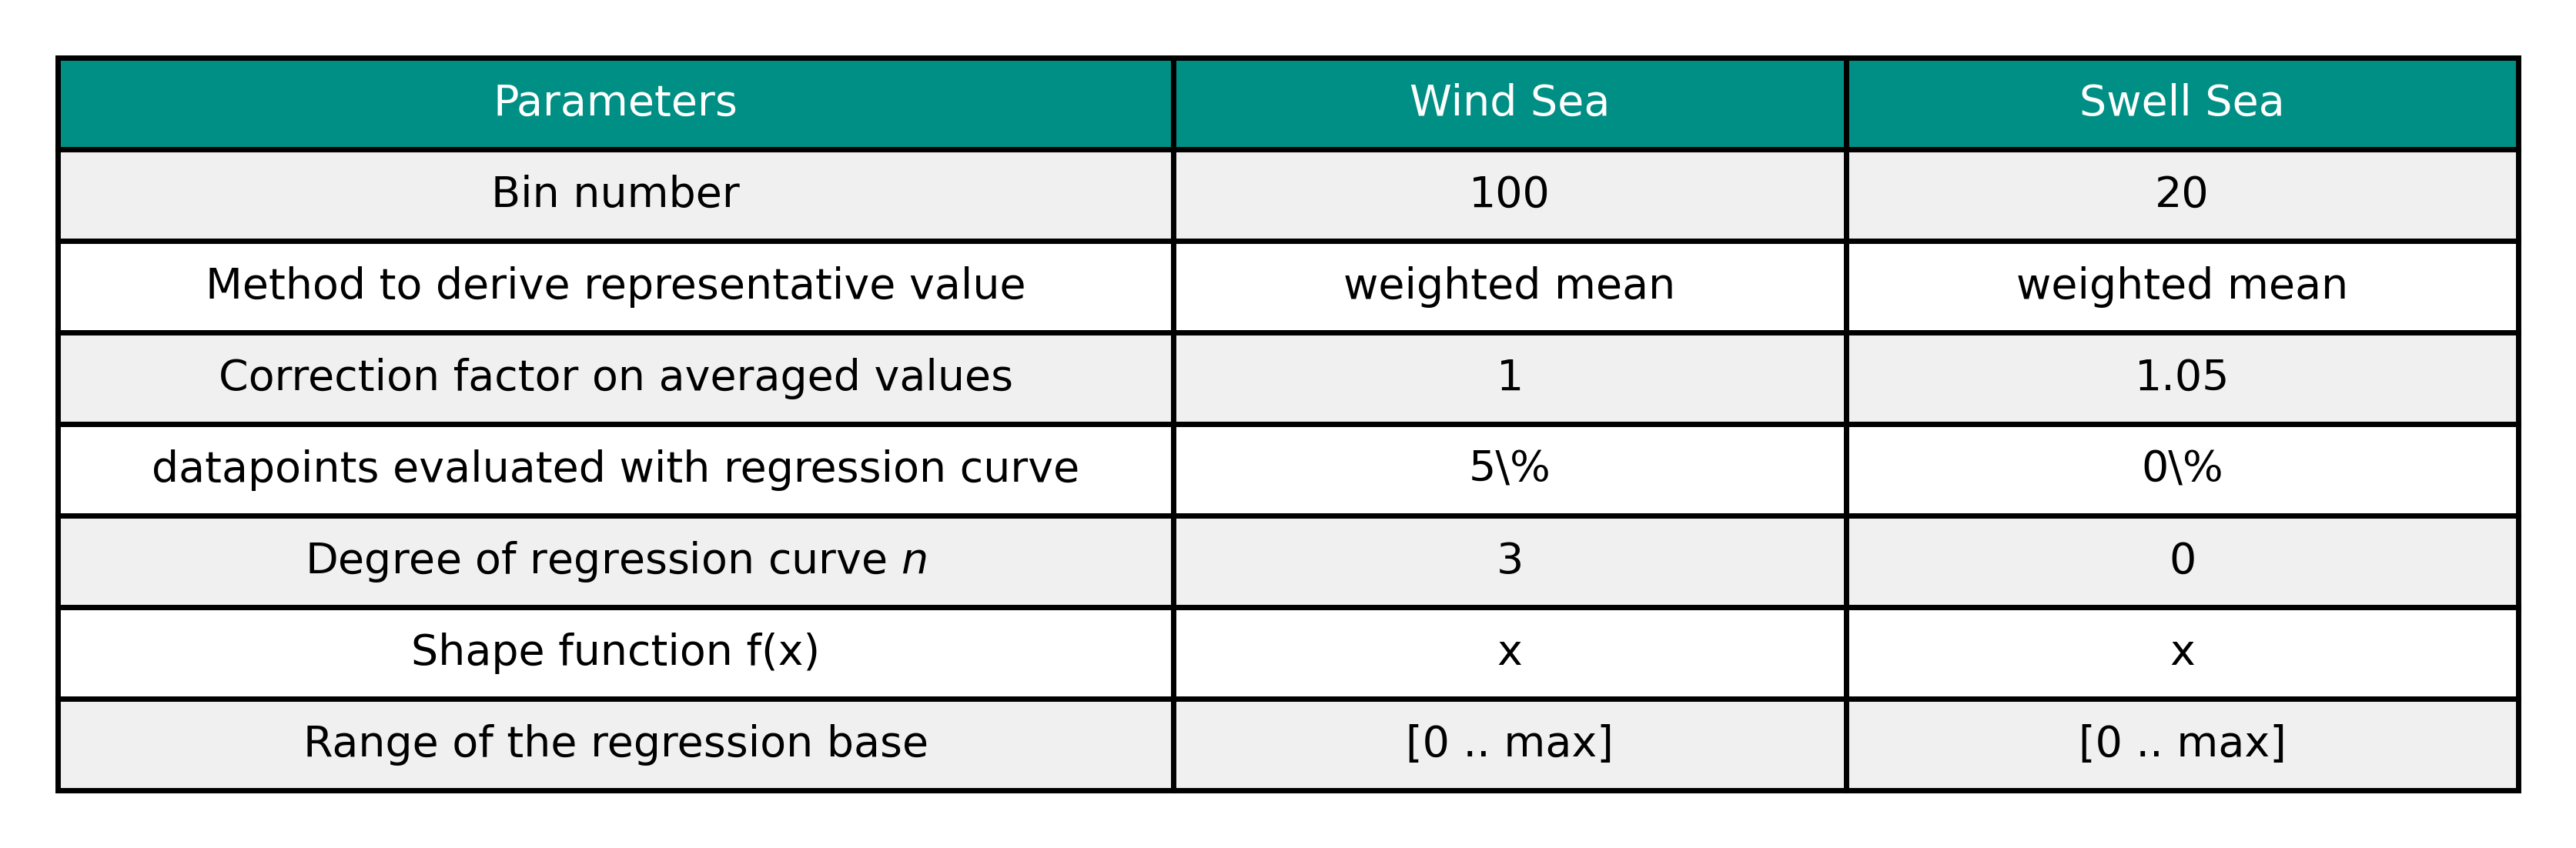
\includegraphics[width=1.0\textwidth ]{C:/Users/aaron.lange/Desktop/Projekte/Hindcast_Tool/HindTool/example_output/Report_table_VMHS_page_1.png} 
 \captionsetup{type=table} 
\caption{ Report-table-VMHS-page-1 } 
 \label{tab: Report_table_VMHS_page_1 } 
\end{figure}

For higher wind speeds and wave heights, the number of datapoints in the hindcast data set decreases. This can lead to representative values for higher bins fluctuating. To mitigate this, a regression analysis is performed. The results from the regression analysis are then used for the higher bins instead of the representative values. The parameter "proportion of datapoints evaluated with regression curve" (Table 6-1 and Table 6-2) specifies how many points of the hindcast set are considered using the regression analysis results rather than the representative values of the bins. The regression analysis is based on a polynomial function of degree $n$ (defined in Table 6-1 and Table 6-2):

$$
\hat{y}(x)=\sum_{i=0}^{n} c_{i} f(x)^{i}
$$

The $x$ values represent either the wind speed (in case of the wind speed to significant wave height condensation) or the wave height (for significant wave height versus peak period) of each bin within the "range of the regression base" (see Table 6-1 and Table 6-2). $\hat{y}$ is the calculated wave height or peak period, respectively. The regression coefficients $c_{\mathrm{i}}$ are determined using a least-squares fit, which minimizes the deviations of $\hat{y}$ to the calculated representative value of each bin. The function $f(x)$ is typically either $x$ or $\sqrt{x}$ and is specified in Table 6-1 and Table 6-2.

Finally, the selected condensation values are a combination of the representative values for the first bins and the values calculated by the regression curve for the higher bins. Note that a regression curve is not always necessary. In such cases, the parameter "proportion of datapoints evaluated with regression curve (highest wind speeds)" is $0 \%$, and all condensation results are derived from the representative values.



\subsubsection{Significant wave height over wind speed}
An equivalent significant wave height vs. wind speed correlation is determined for the omnidirectional case and the directional distribution. The following weighting approach is applied:

$$
H_{s, e q}=\left(\frac{\sum_{n} H_{s, n}{ }^{\lambda m} \cdot p(n)}{\sum_{n} p(n)}\right)^{\frac{1}{\lambda m}}
$$

Here, $\lambda$ is chosen to be 1 as wave loads on monopiles are inertia dominated (see also [L2]), whereas $m$ shall be equal to 2 and denotes the power mean exponent. This approach is solely based on the conservation of the wave energy of a sea state or the corresponding spectrum, respectively. The wave energy of a linear sea state is proportional to the square of significant wave height $\left(E \sim H_{S}^{2}\right)$.

The calculated condensation curve is adjusted to ensure it forms a monotone increasing function. This means that as wind speeds increase, the $H_{S}$ either increases or remains constant. This is physically obvious but can be calculated differently for high bins due to a lack of data.

The condensation is calculated using the following parameters in REF.\\
REF: Condensation parameter wind speed versus significant wave height
 
\begin{figure}[H] 
 \centering 
 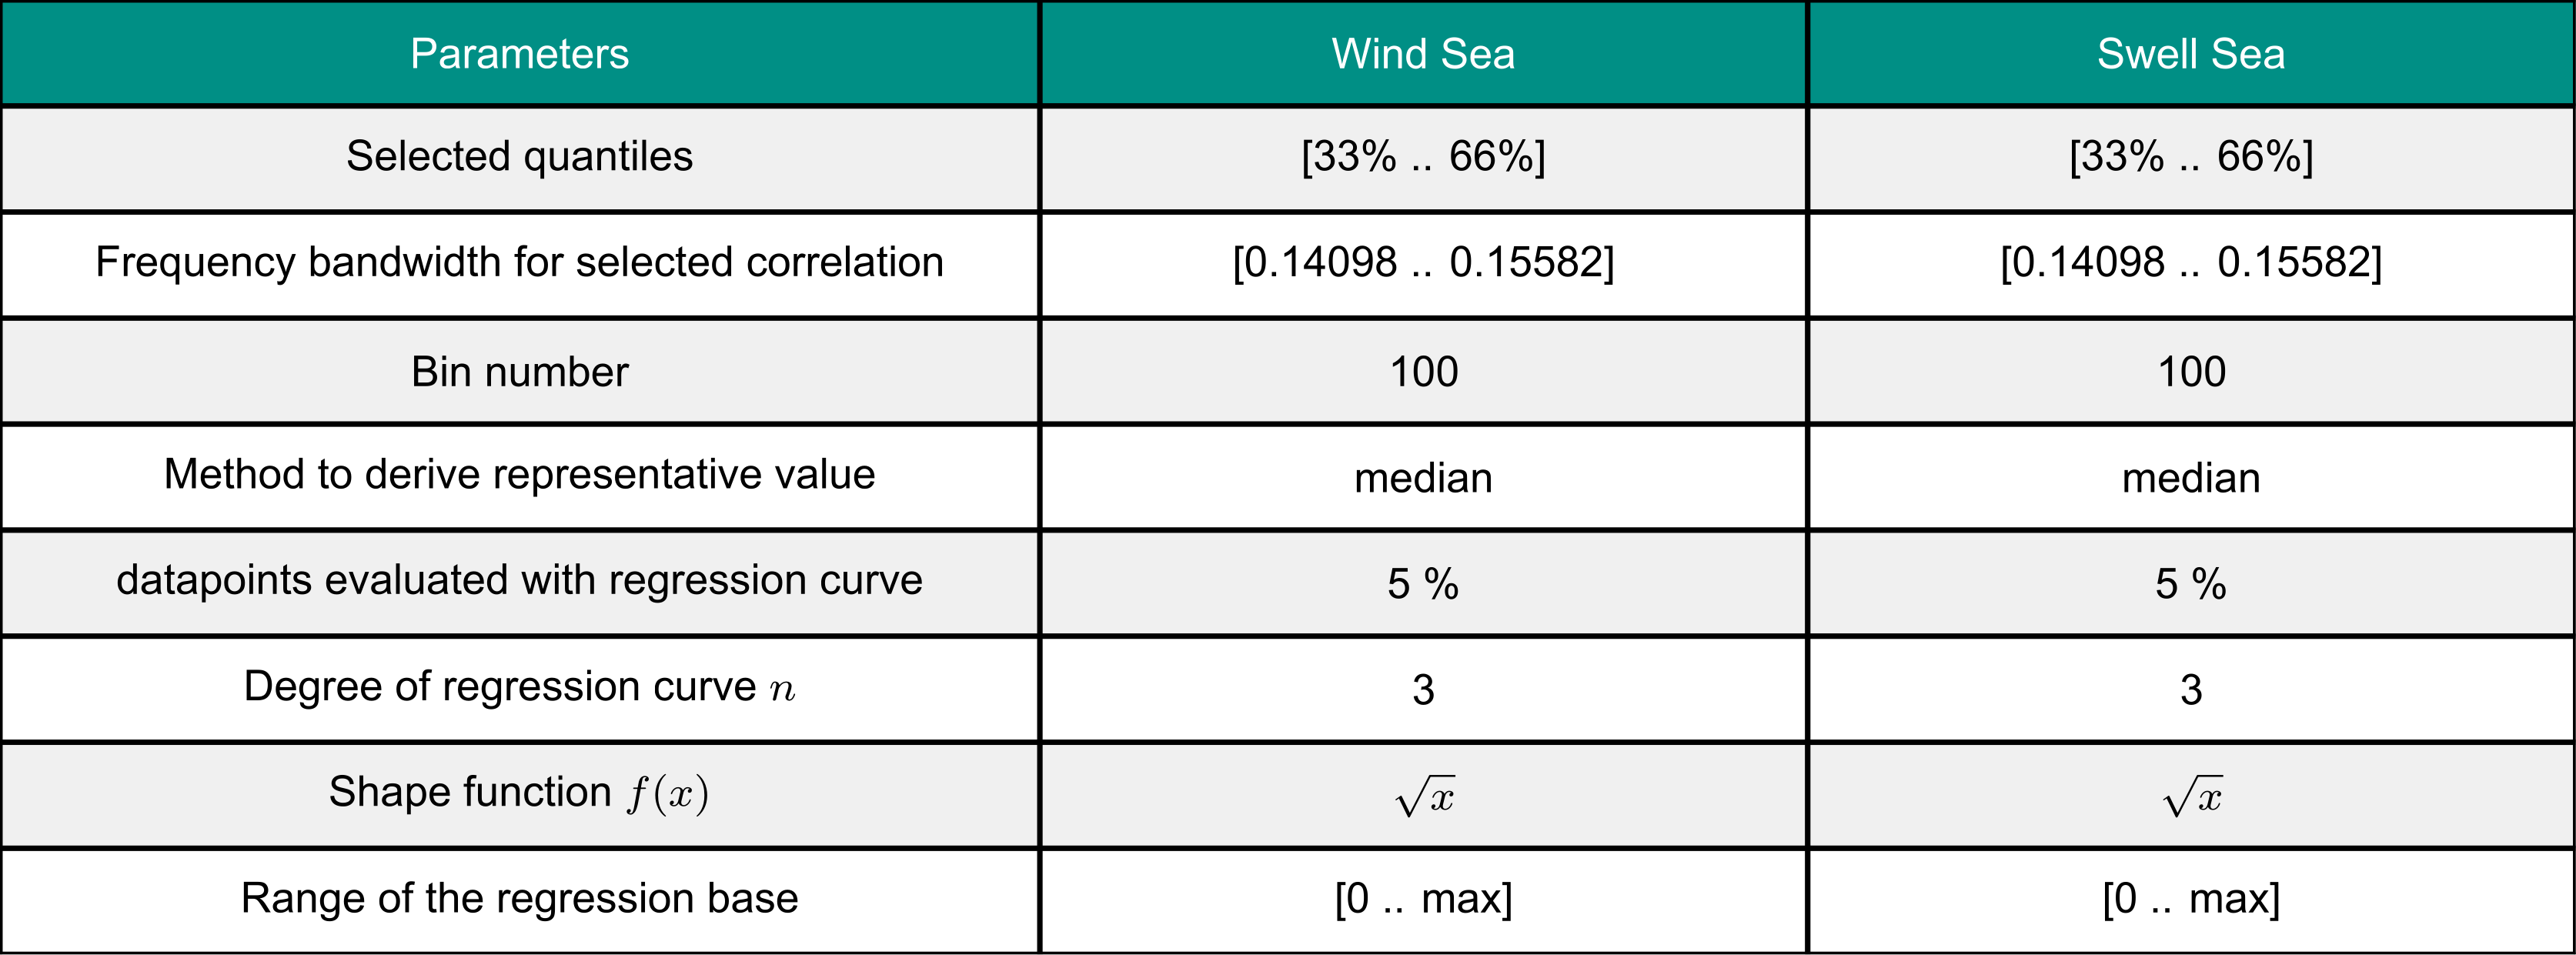
\includegraphics[width=1.0\textwidth ]{C:/Users/aaron.lange/Desktop/Projekte/Hindcast_Tool/HindTool/example_output/Report_table_HSTP_page_1.png} 
 \captionsetup{type=table} 
\caption{ Report-table-HSTP-page-1 } 
 \label{tab: Report_table_HSTP_page_1 } 
\end{figure}

The result for the omnidirectional wind sea case is shown REF. Results for each sector are listed in Fehler! Verweisquelle konnte nicht gefunden werden.\\
omnidirectional\\

\begin{figure}[H] 
 \centering 
 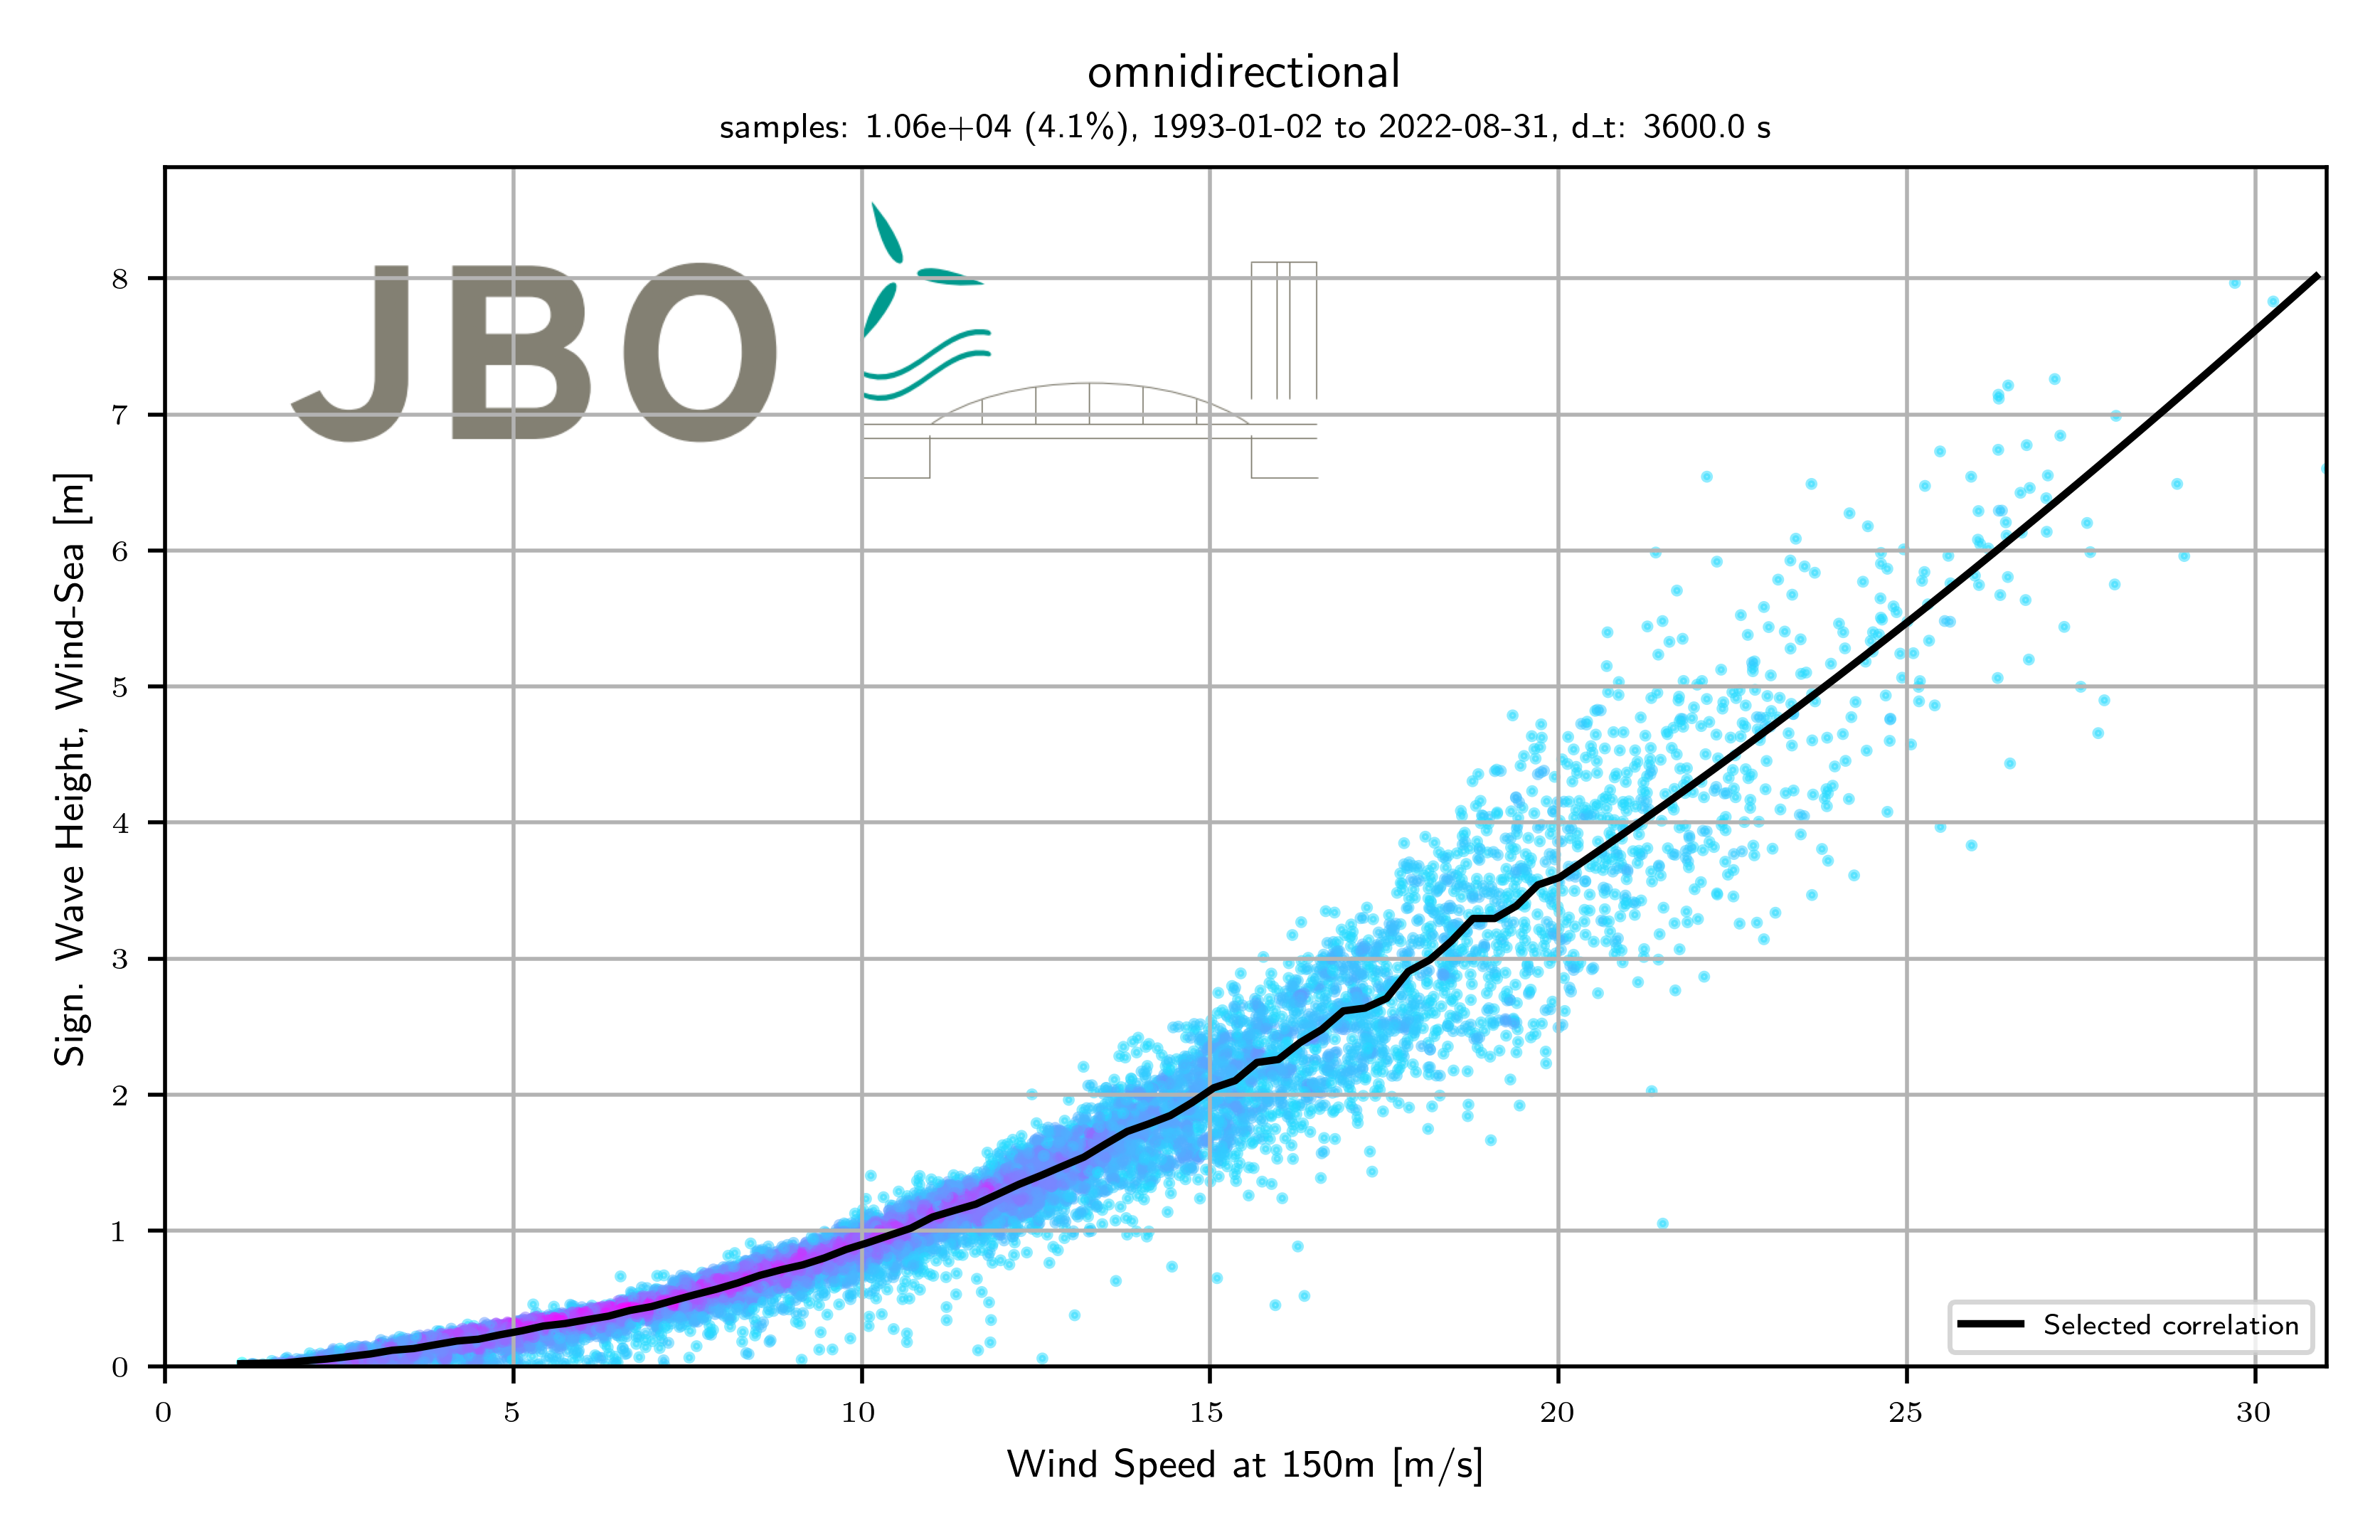
\includegraphics[width=1.0\textwidth]{C:/Users/aaron.lange/Desktop/Projekte/Hindcast_Tool/HindTool/example_output/VMHS_wind_page_3.png} 
 \caption{ VMHS-wind-page-3 } 
 \label{fig: VMHS_wind_page_3 } 
\end{figure}
\begin{figure}[H] 
 \centering 
 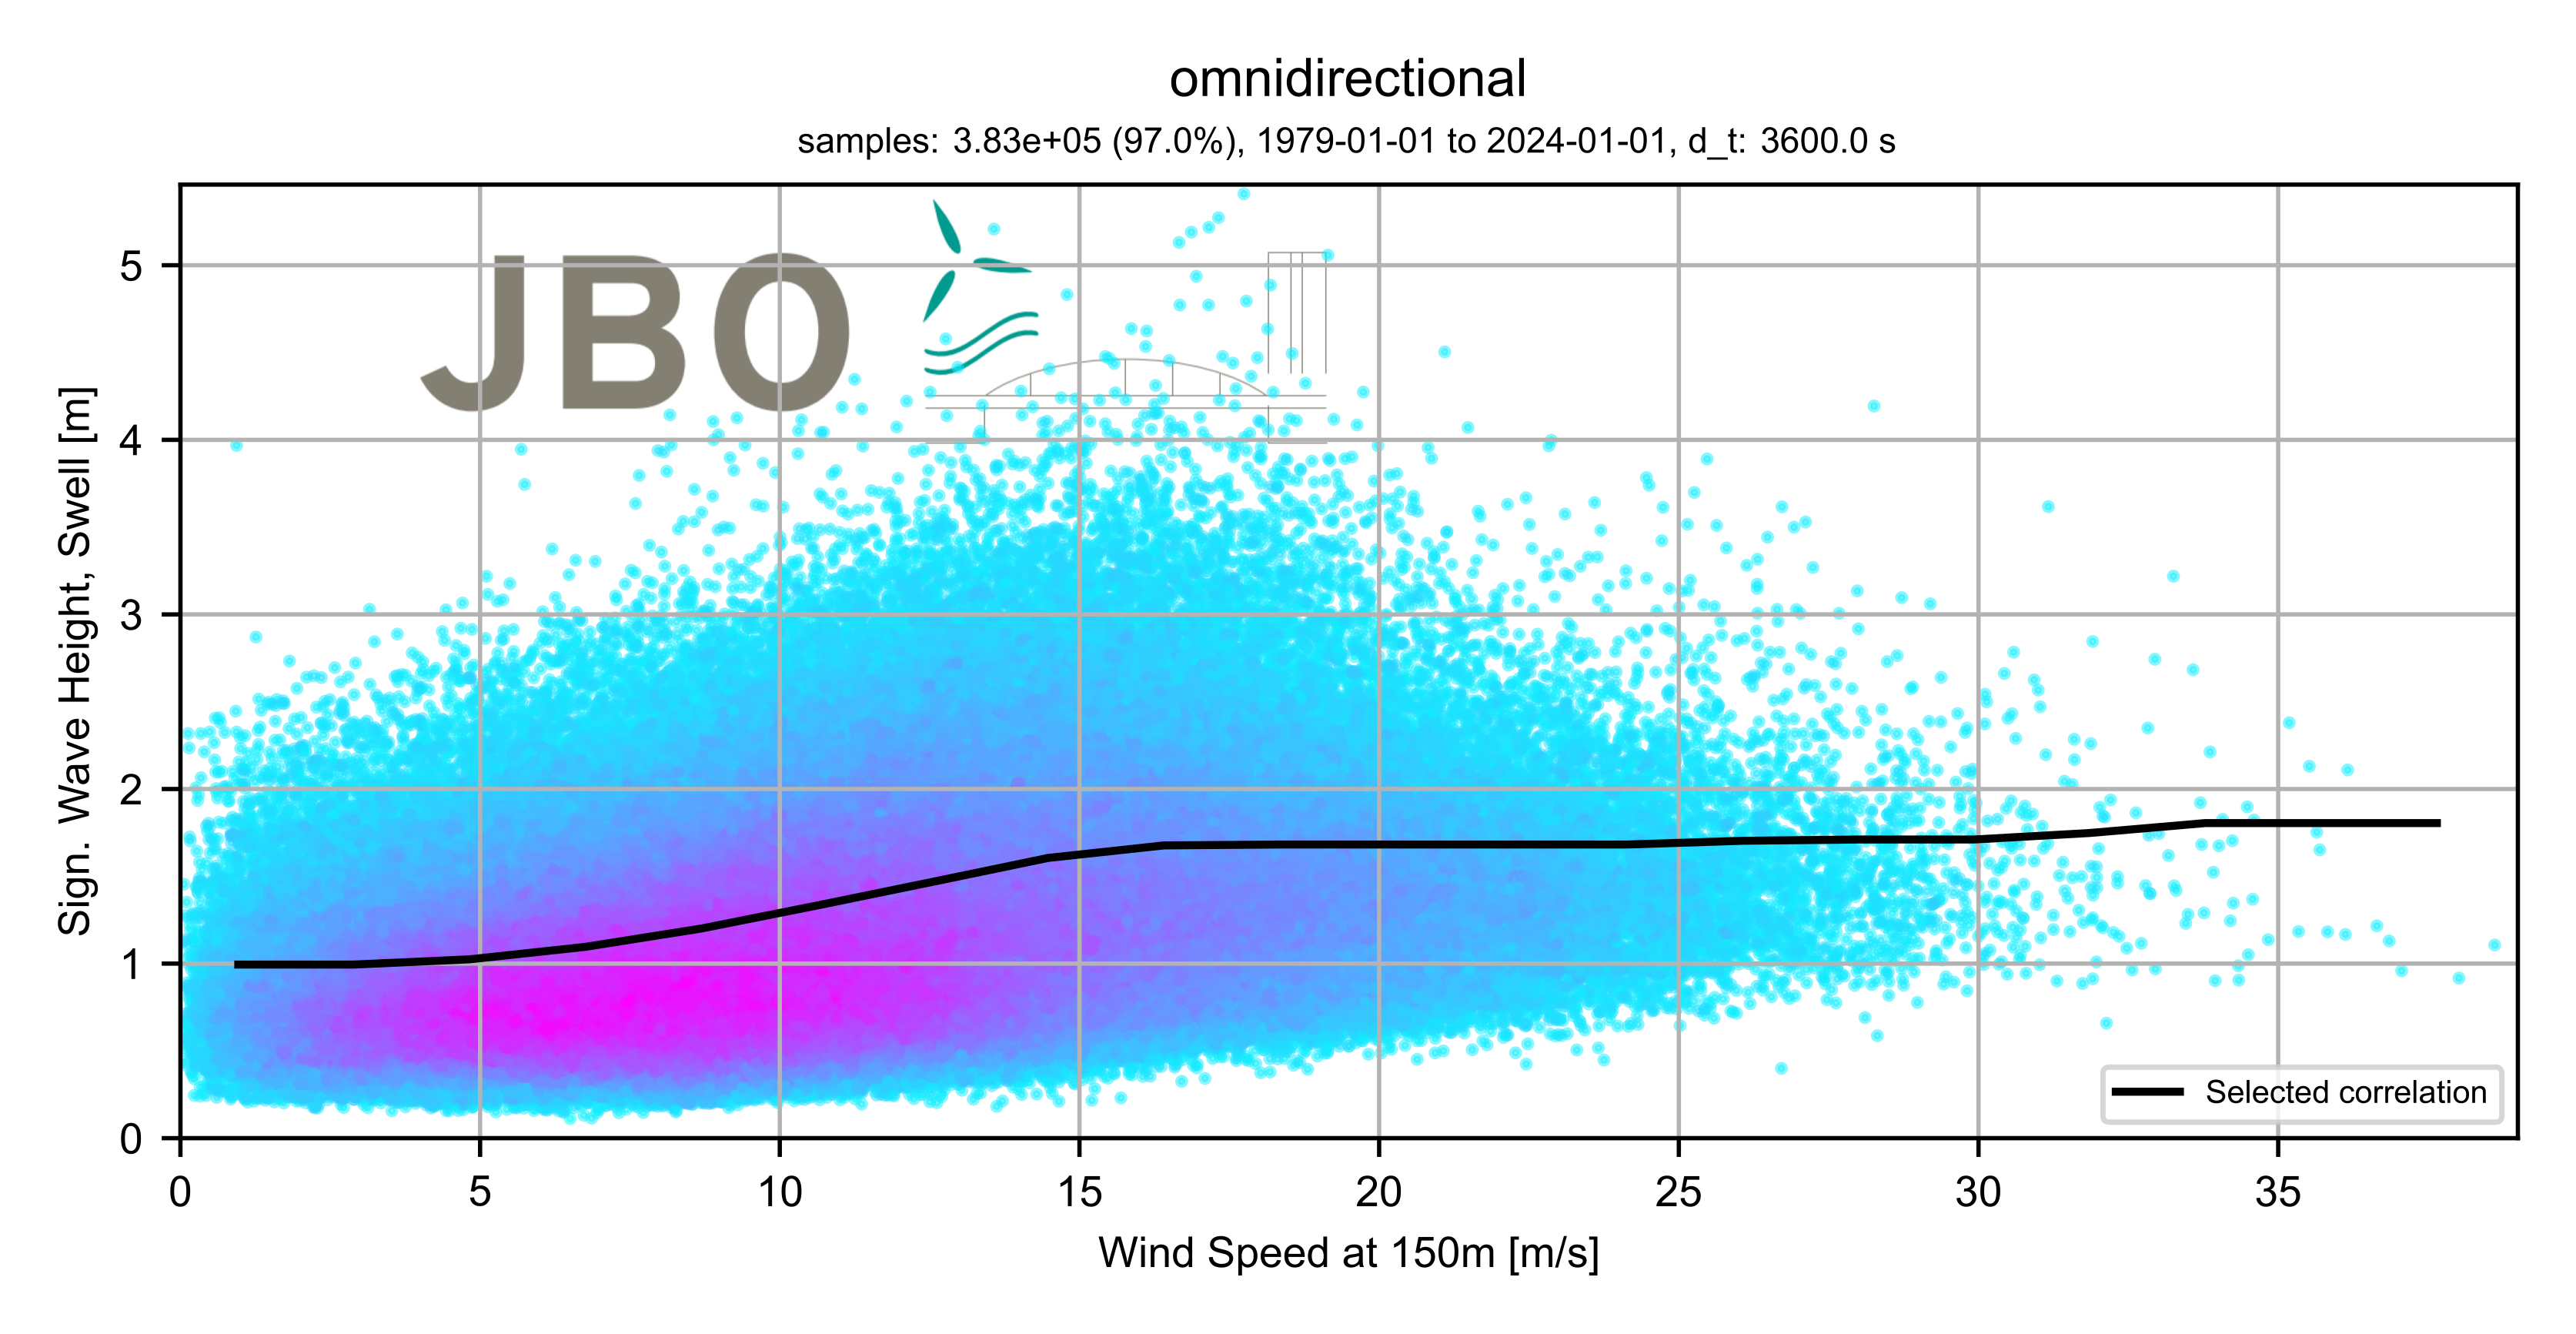
\includegraphics[width=1.0\textwidth]{C:/Users/aaron.lange/Desktop/Projekte/Hindcast_Tool/HindTool/example_output/VMHS_swell_page_3.png} 
 \caption{ VMHS-swell-page-3 } 
 \label{fig: VMHS_swell_page_3 } 
\end{figure}

\begin{figure}[H] 
 \centering 
 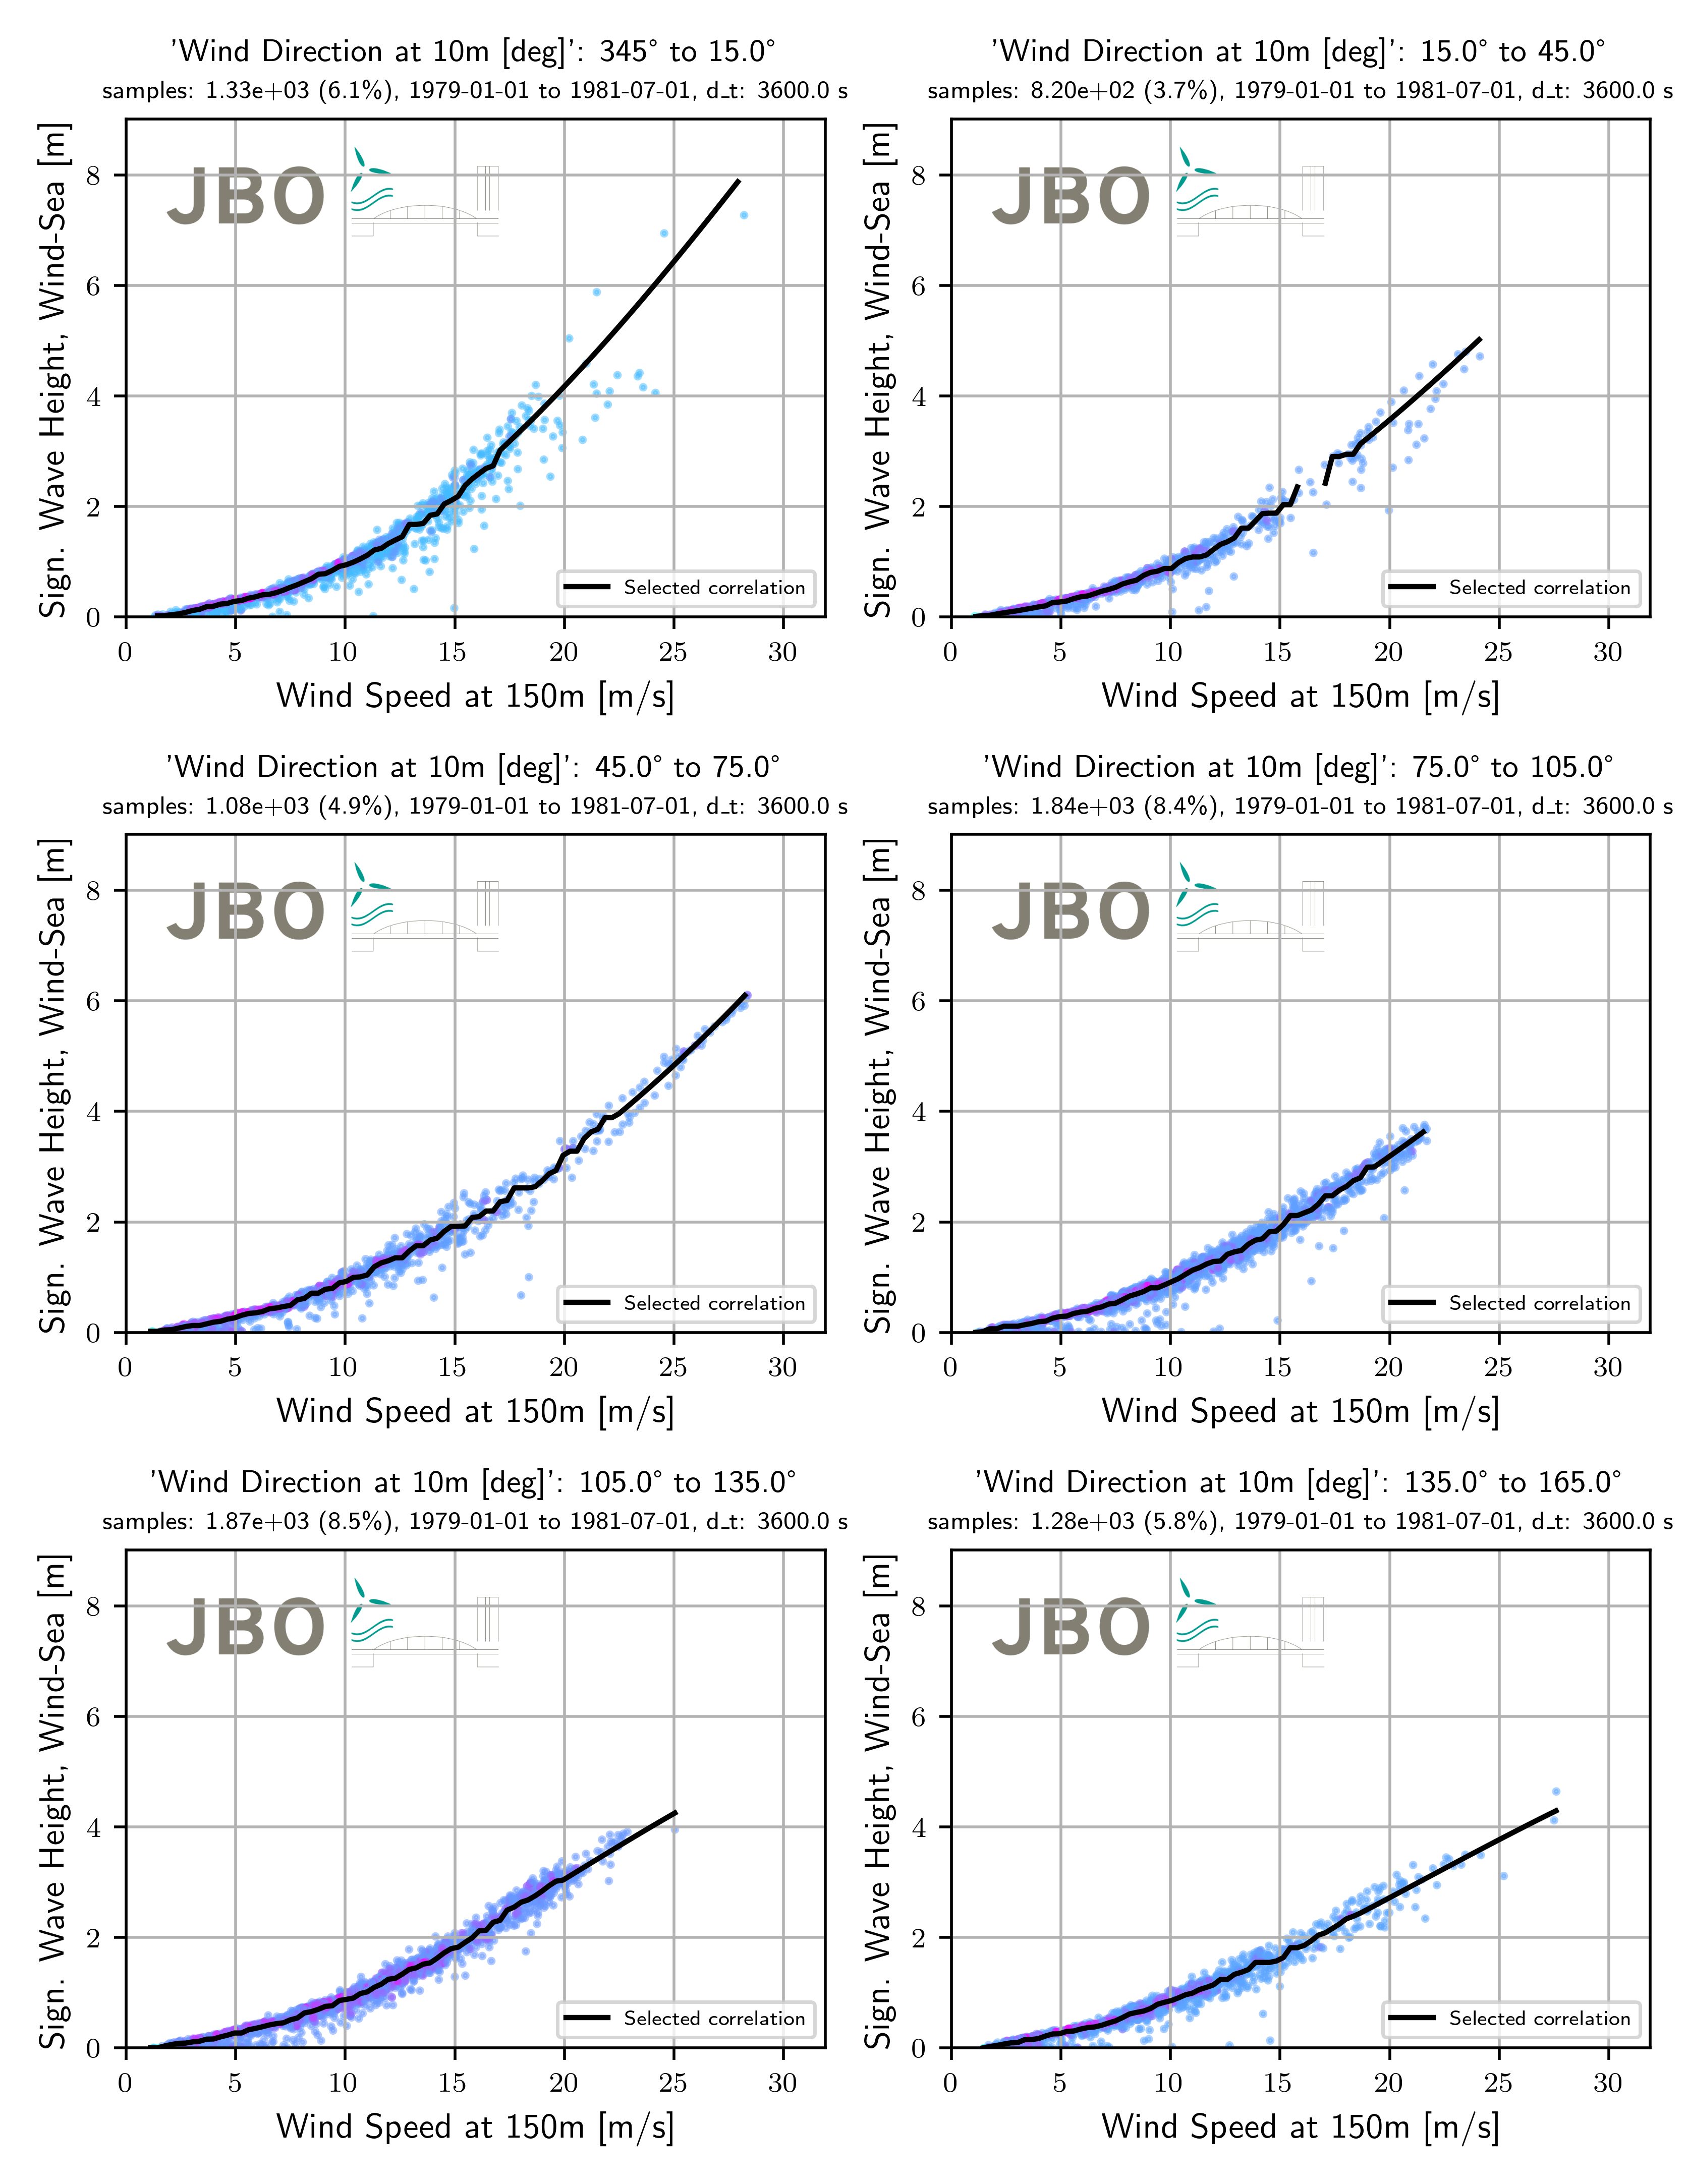
\includegraphics[width=1.0\textwidth]{C:/Users/aaron.lange/Desktop/Projekte/Hindcast_Tool/HindTool/example_output/VMHS_wind_page_1.png} 
 \caption{ VMHS-wind-page-1 } 
 \label{fig: VMHS_wind_page_1 } 
\end{figure}
\begin{figure}[H] 
 \centering 
 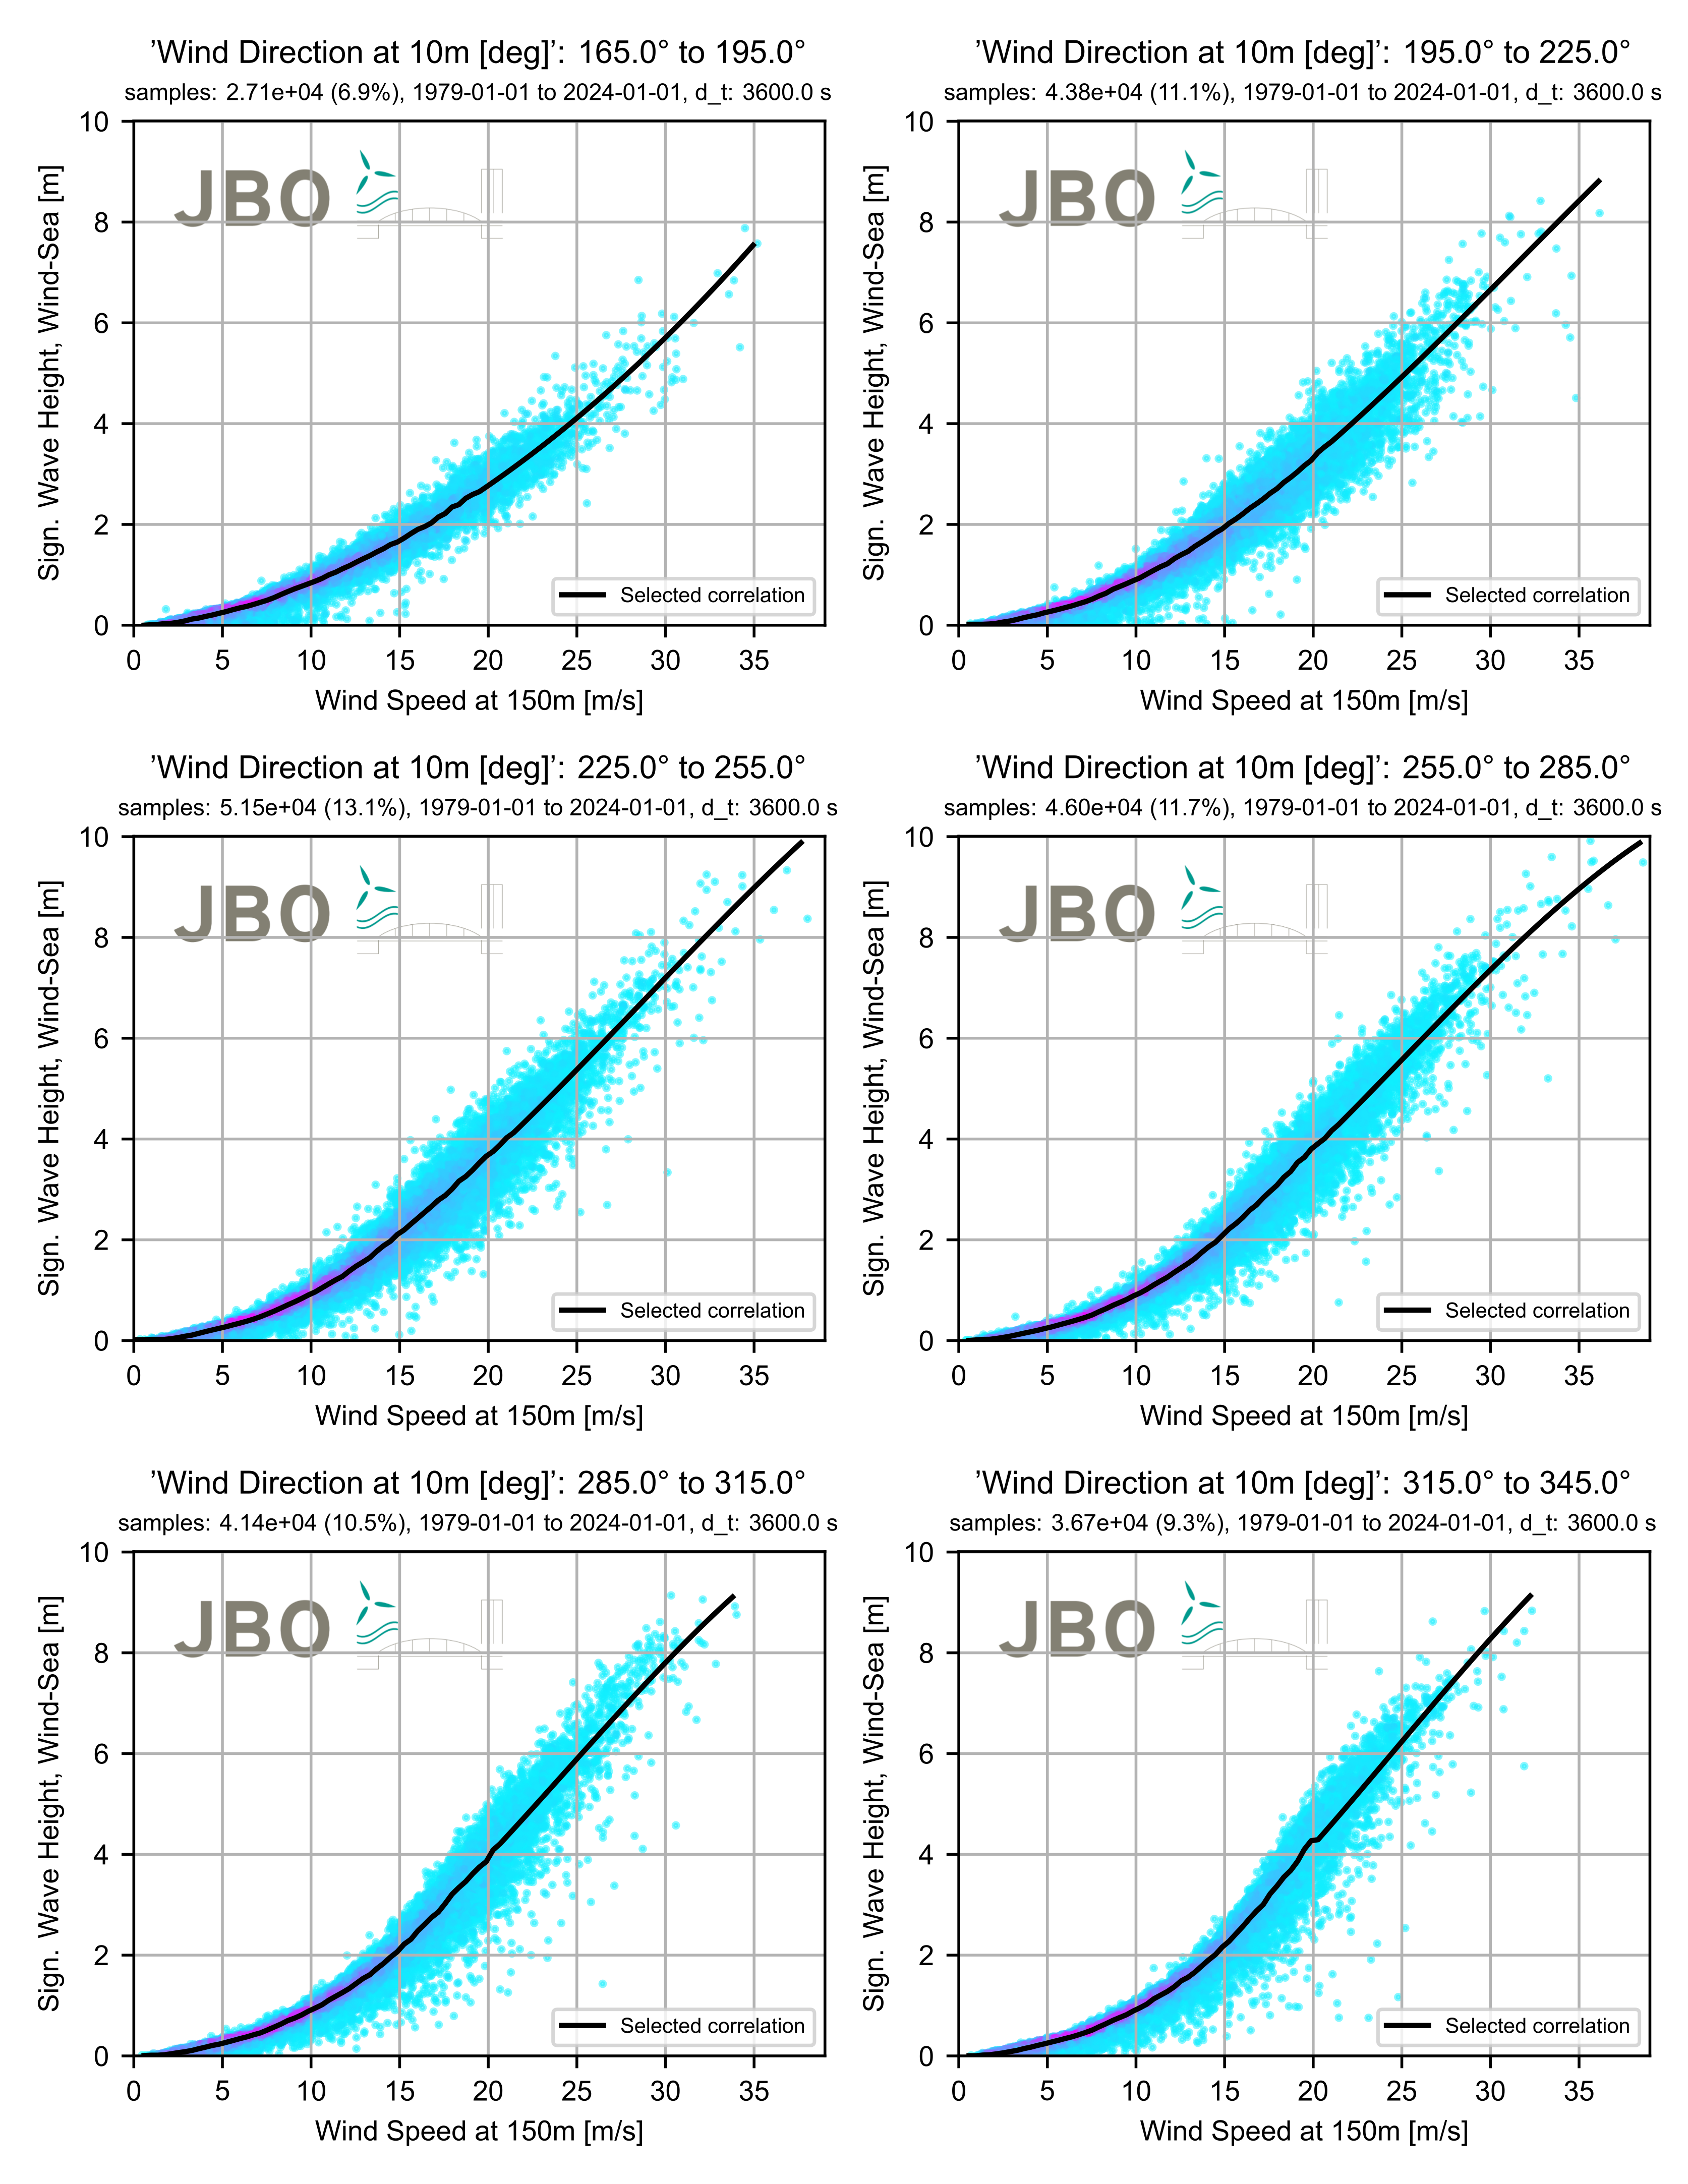
\includegraphics[width=1.0\textwidth]{C:/Users/aaron.lange/Desktop/Projekte/Hindcast_Tool/HindTool/example_output/VMHS_wind_page_2.png} 
 \caption{ VMHS-wind-page-2 } 
 \label{fig: VMHS_wind_page_2 } 
\end{figure}

\begin{figure}[H] 
 \centering 
 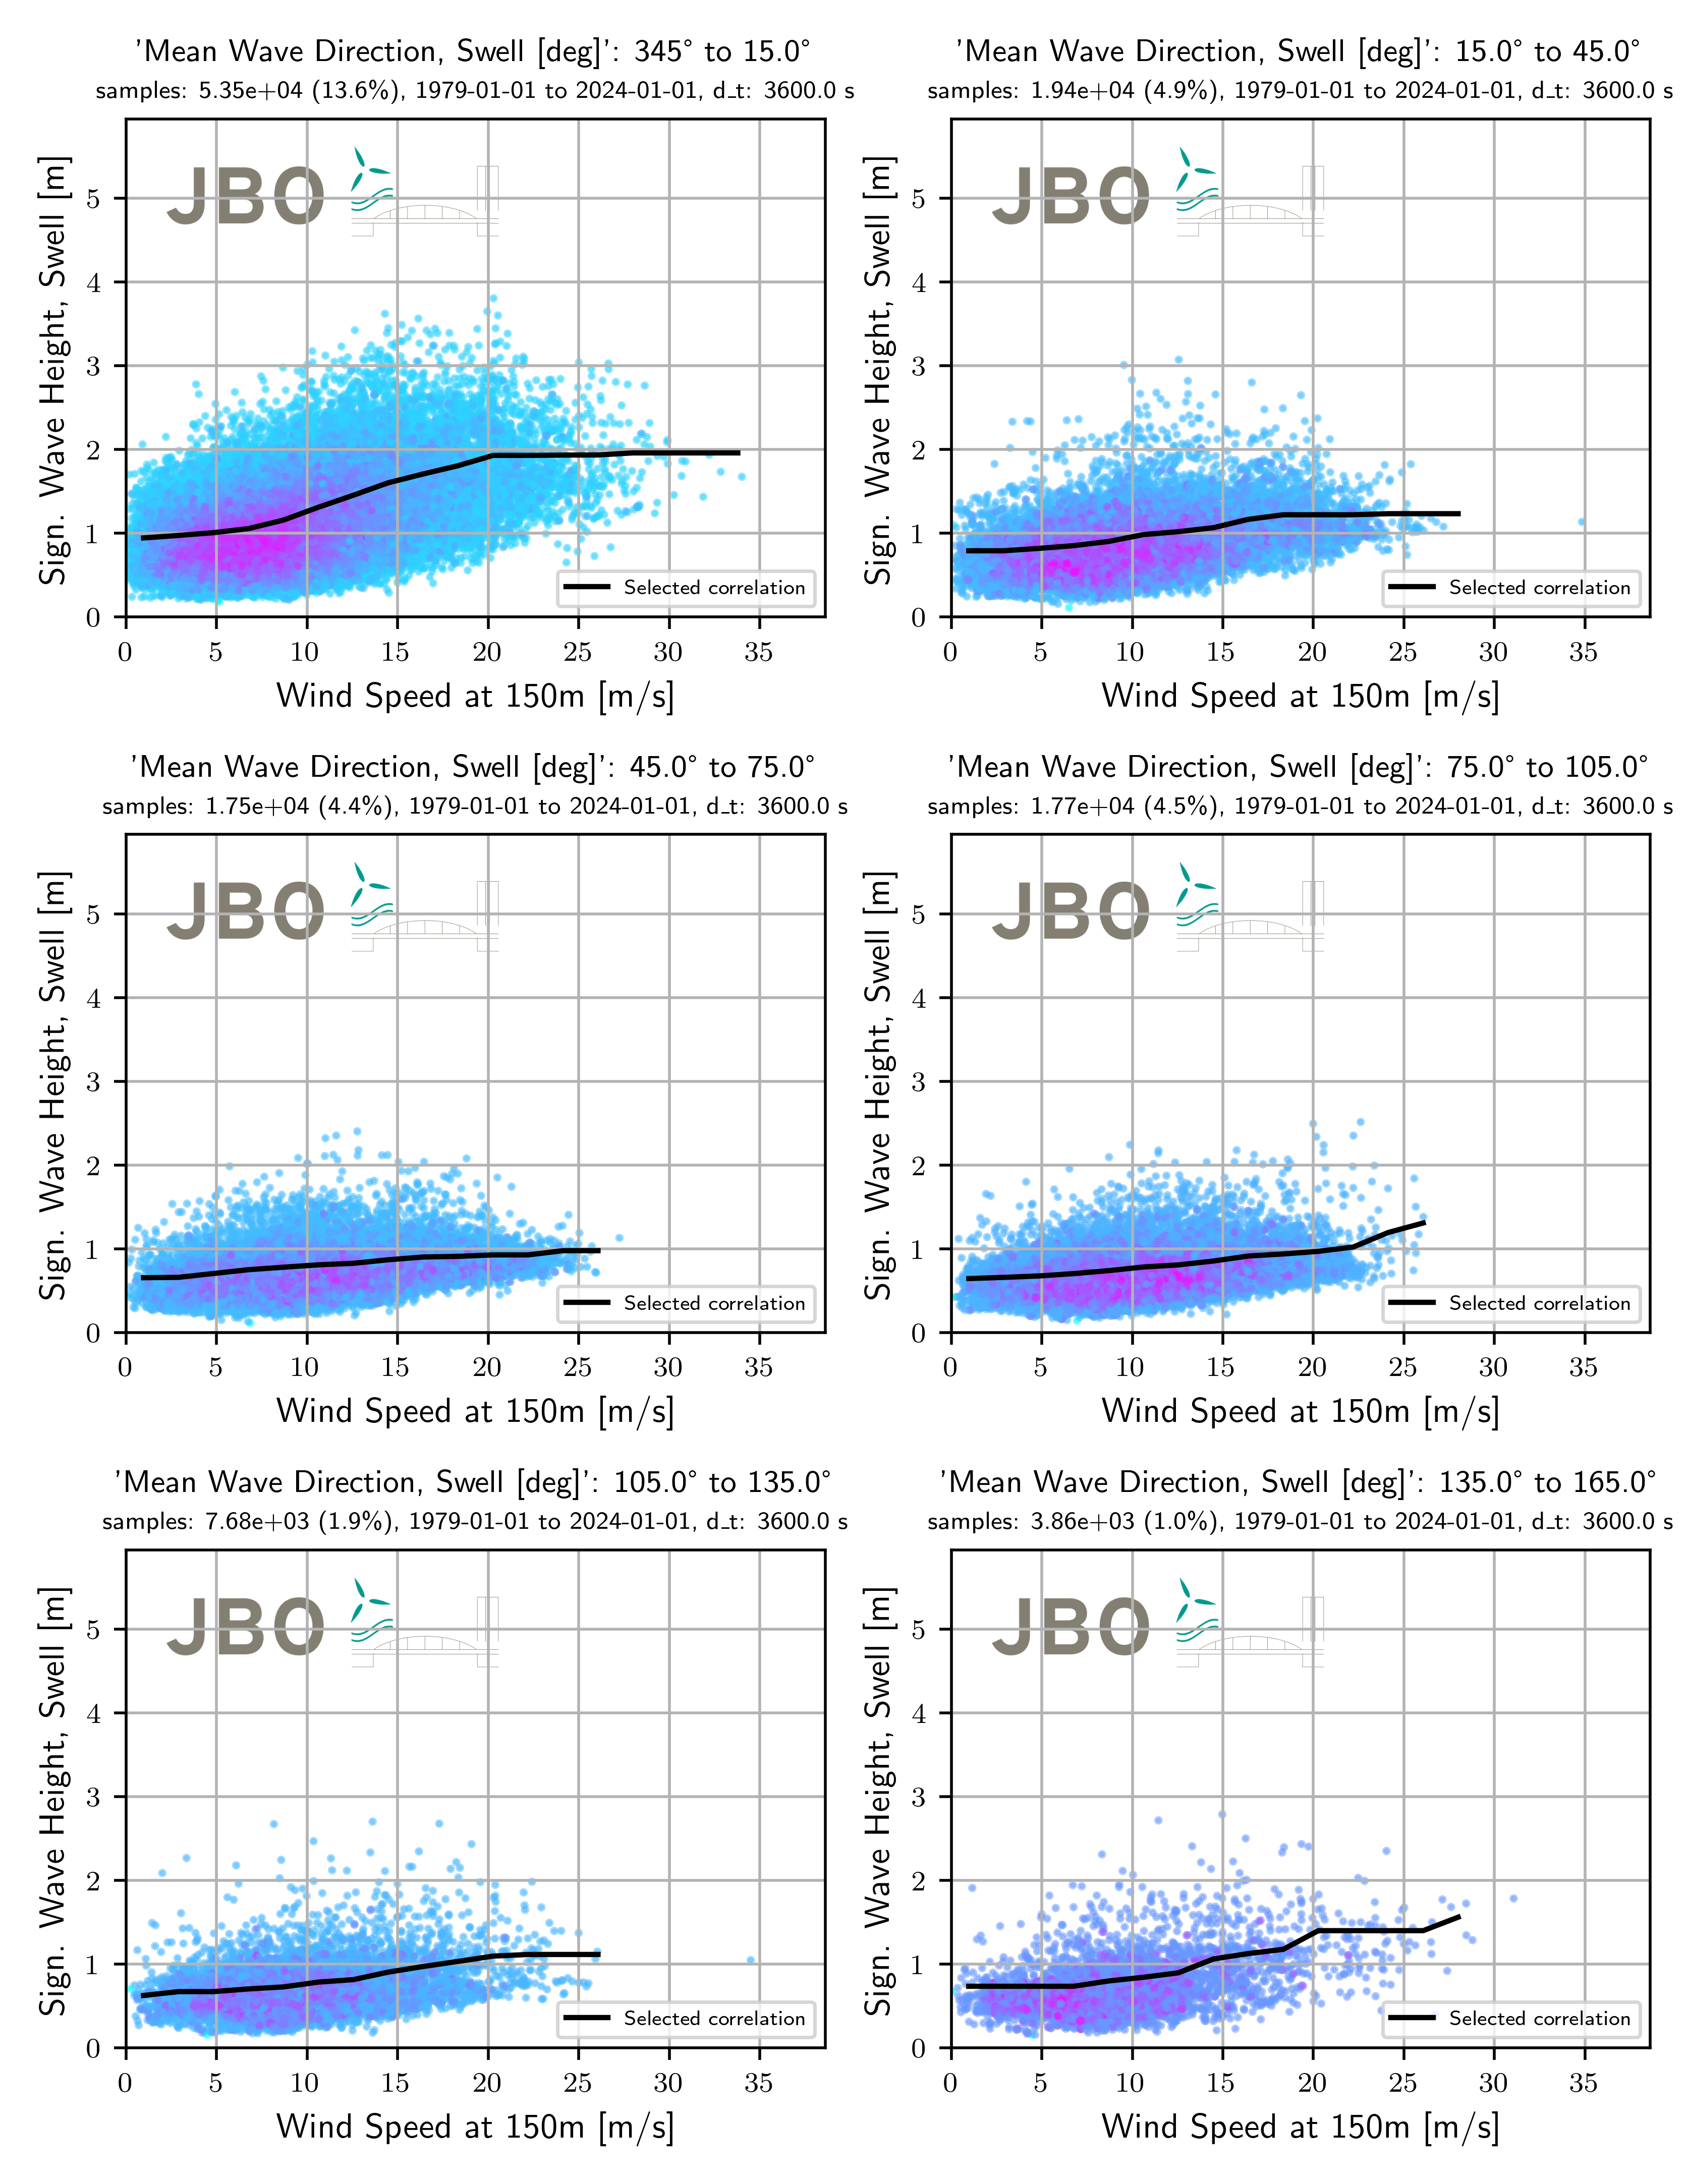
\includegraphics[width=1.0\textwidth]{C:/Users/aaron.lange/Desktop/Projekte/Hindcast_Tool/HindTool/example_output/VMHS_swell_page_1.png} 
 \caption{ VMHS-swell-page-1 } 
 \label{fig: VMHS_swell_page_1 } 
\end{figure}
\begin{figure}[H] 
 \centering 
 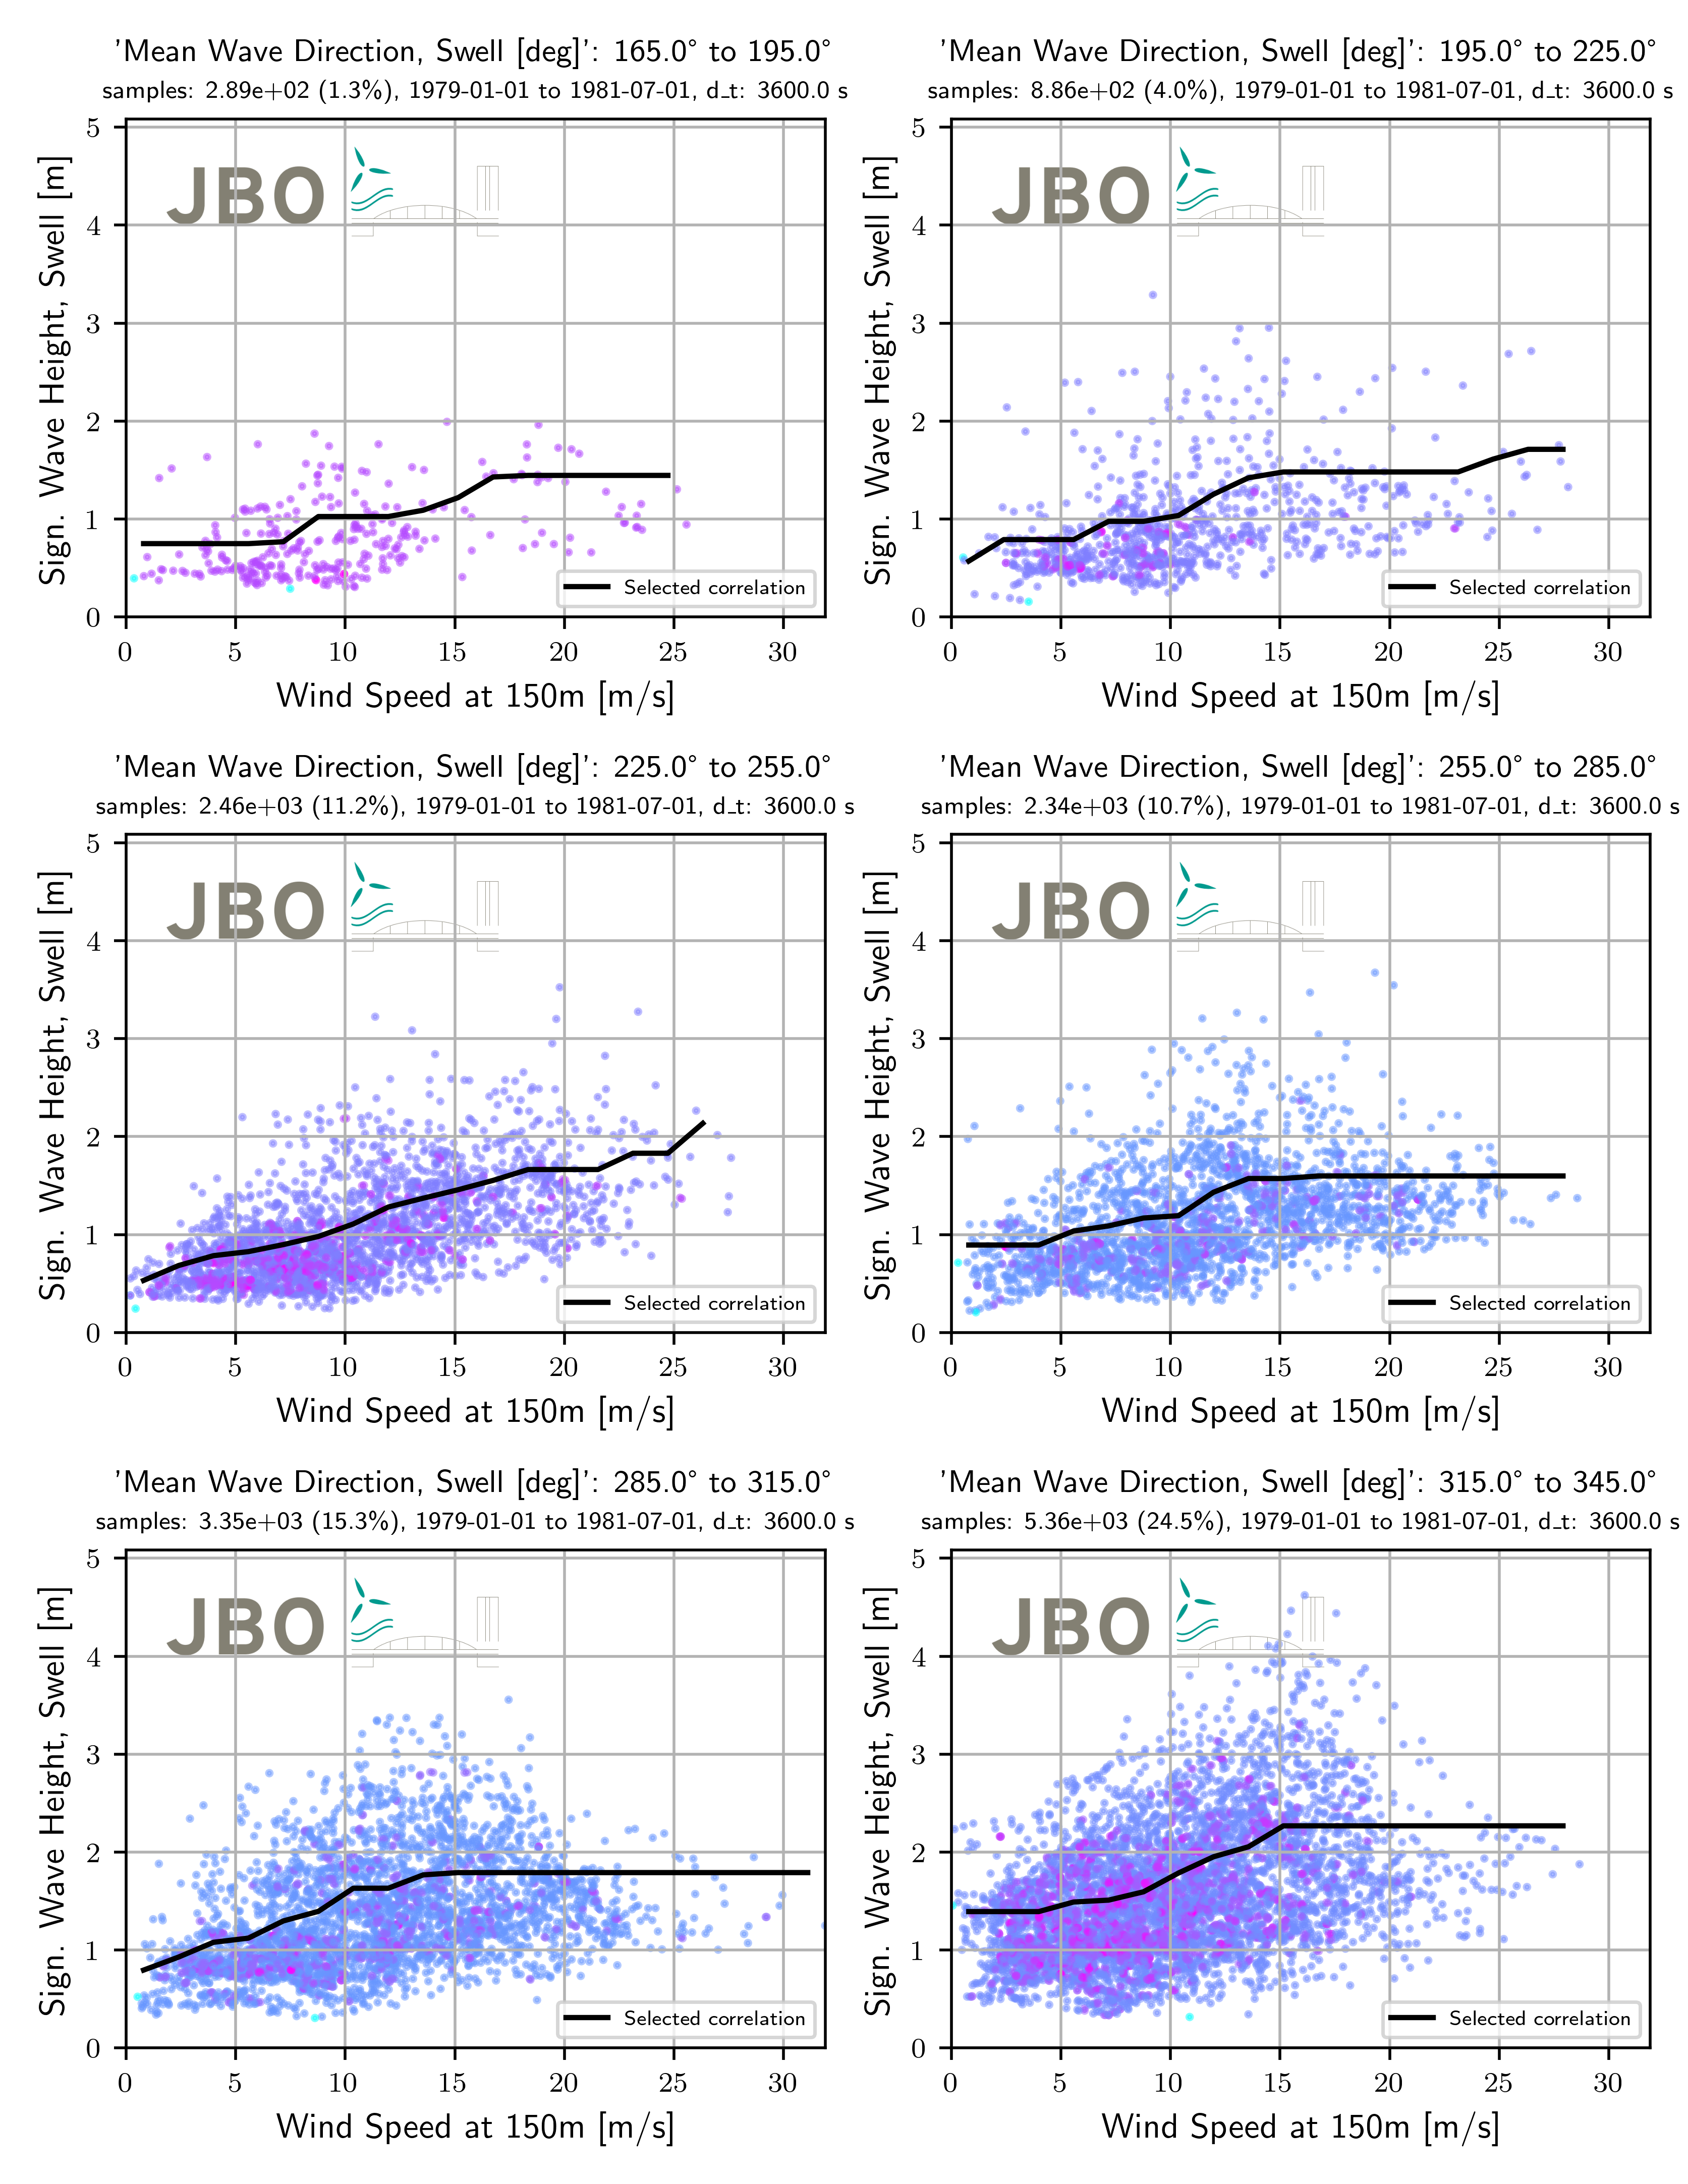
\includegraphics[width=1.0\textwidth]{C:/Users/aaron.lange/Desktop/Projekte/Hindcast_Tool/HindTool/example_output/VMHS_swell_page_2.png} 
 \caption{ VMHS-swell-page-2 } 
 \label{fig: VMHS_swell_page_2 } 
\end{figure}


\subsubsection{Peak period over wind speed }
The cross correlation of the $T_{P}$ data to the $v_{m}$ data is needed, as it forms a sea state with corresponding $H_{S}$ data in the respective $v_{m}$-bin and directional sector. A direct correlation following from a representative value and a regression curve follows no underlying physical connection. Therefore the $v_{m}\left(T_{P}\right)$ relation is derived using the determined correlations $H_{s}\left(v_{m}\right)$ and $T_{P}\left(H_{S}\right)$.

For this, the function $H_{s}\left(v_{m}\right)$ (REF, left) is inverted to $v_{m}\left(H_{S}\right)$ (middle). This is possible because the function is bijective. The goal is to substitute this relation for $H_{S}$ in the $T_{P}\left(H_{S}\right)$ function to get to the correlation of $T_{P}\left(v_{m}\right)$. As shown, the $H_{S}$-values in the horizontal axis aren't equidistant anymore as they are in the $T_{P}\left(H_{S}\right)$ relation. Therefore, new $v_{m}$-values must be interpolated to the appropriate $H_{S}$-values (middle). Now $H_{S}$ can be substituted for $v_{m}$ - and the $T_{P}\left(v_{m}\right)$ relation can be found (right).\\

\begin{figure}[H] 
 \centering 
 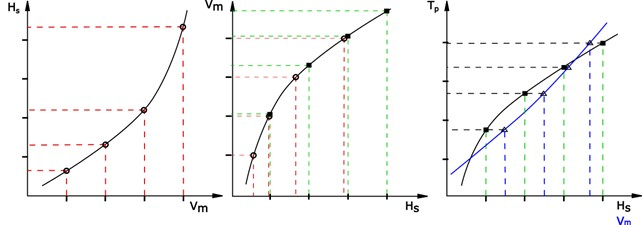
\includegraphics[width=1.0\textwidth]{C:/Users/aaron.lange/Desktop/Projekte/Hindcast_Tool/HindTool/latex_templates/VMTP_theory.jpg} 
 \caption{ Cross correlation for determining peak period over wind speed } 
 \label{fig: VMTP_theory } 
\end{figure}
\begin{figure}[H] 
 \centering 
 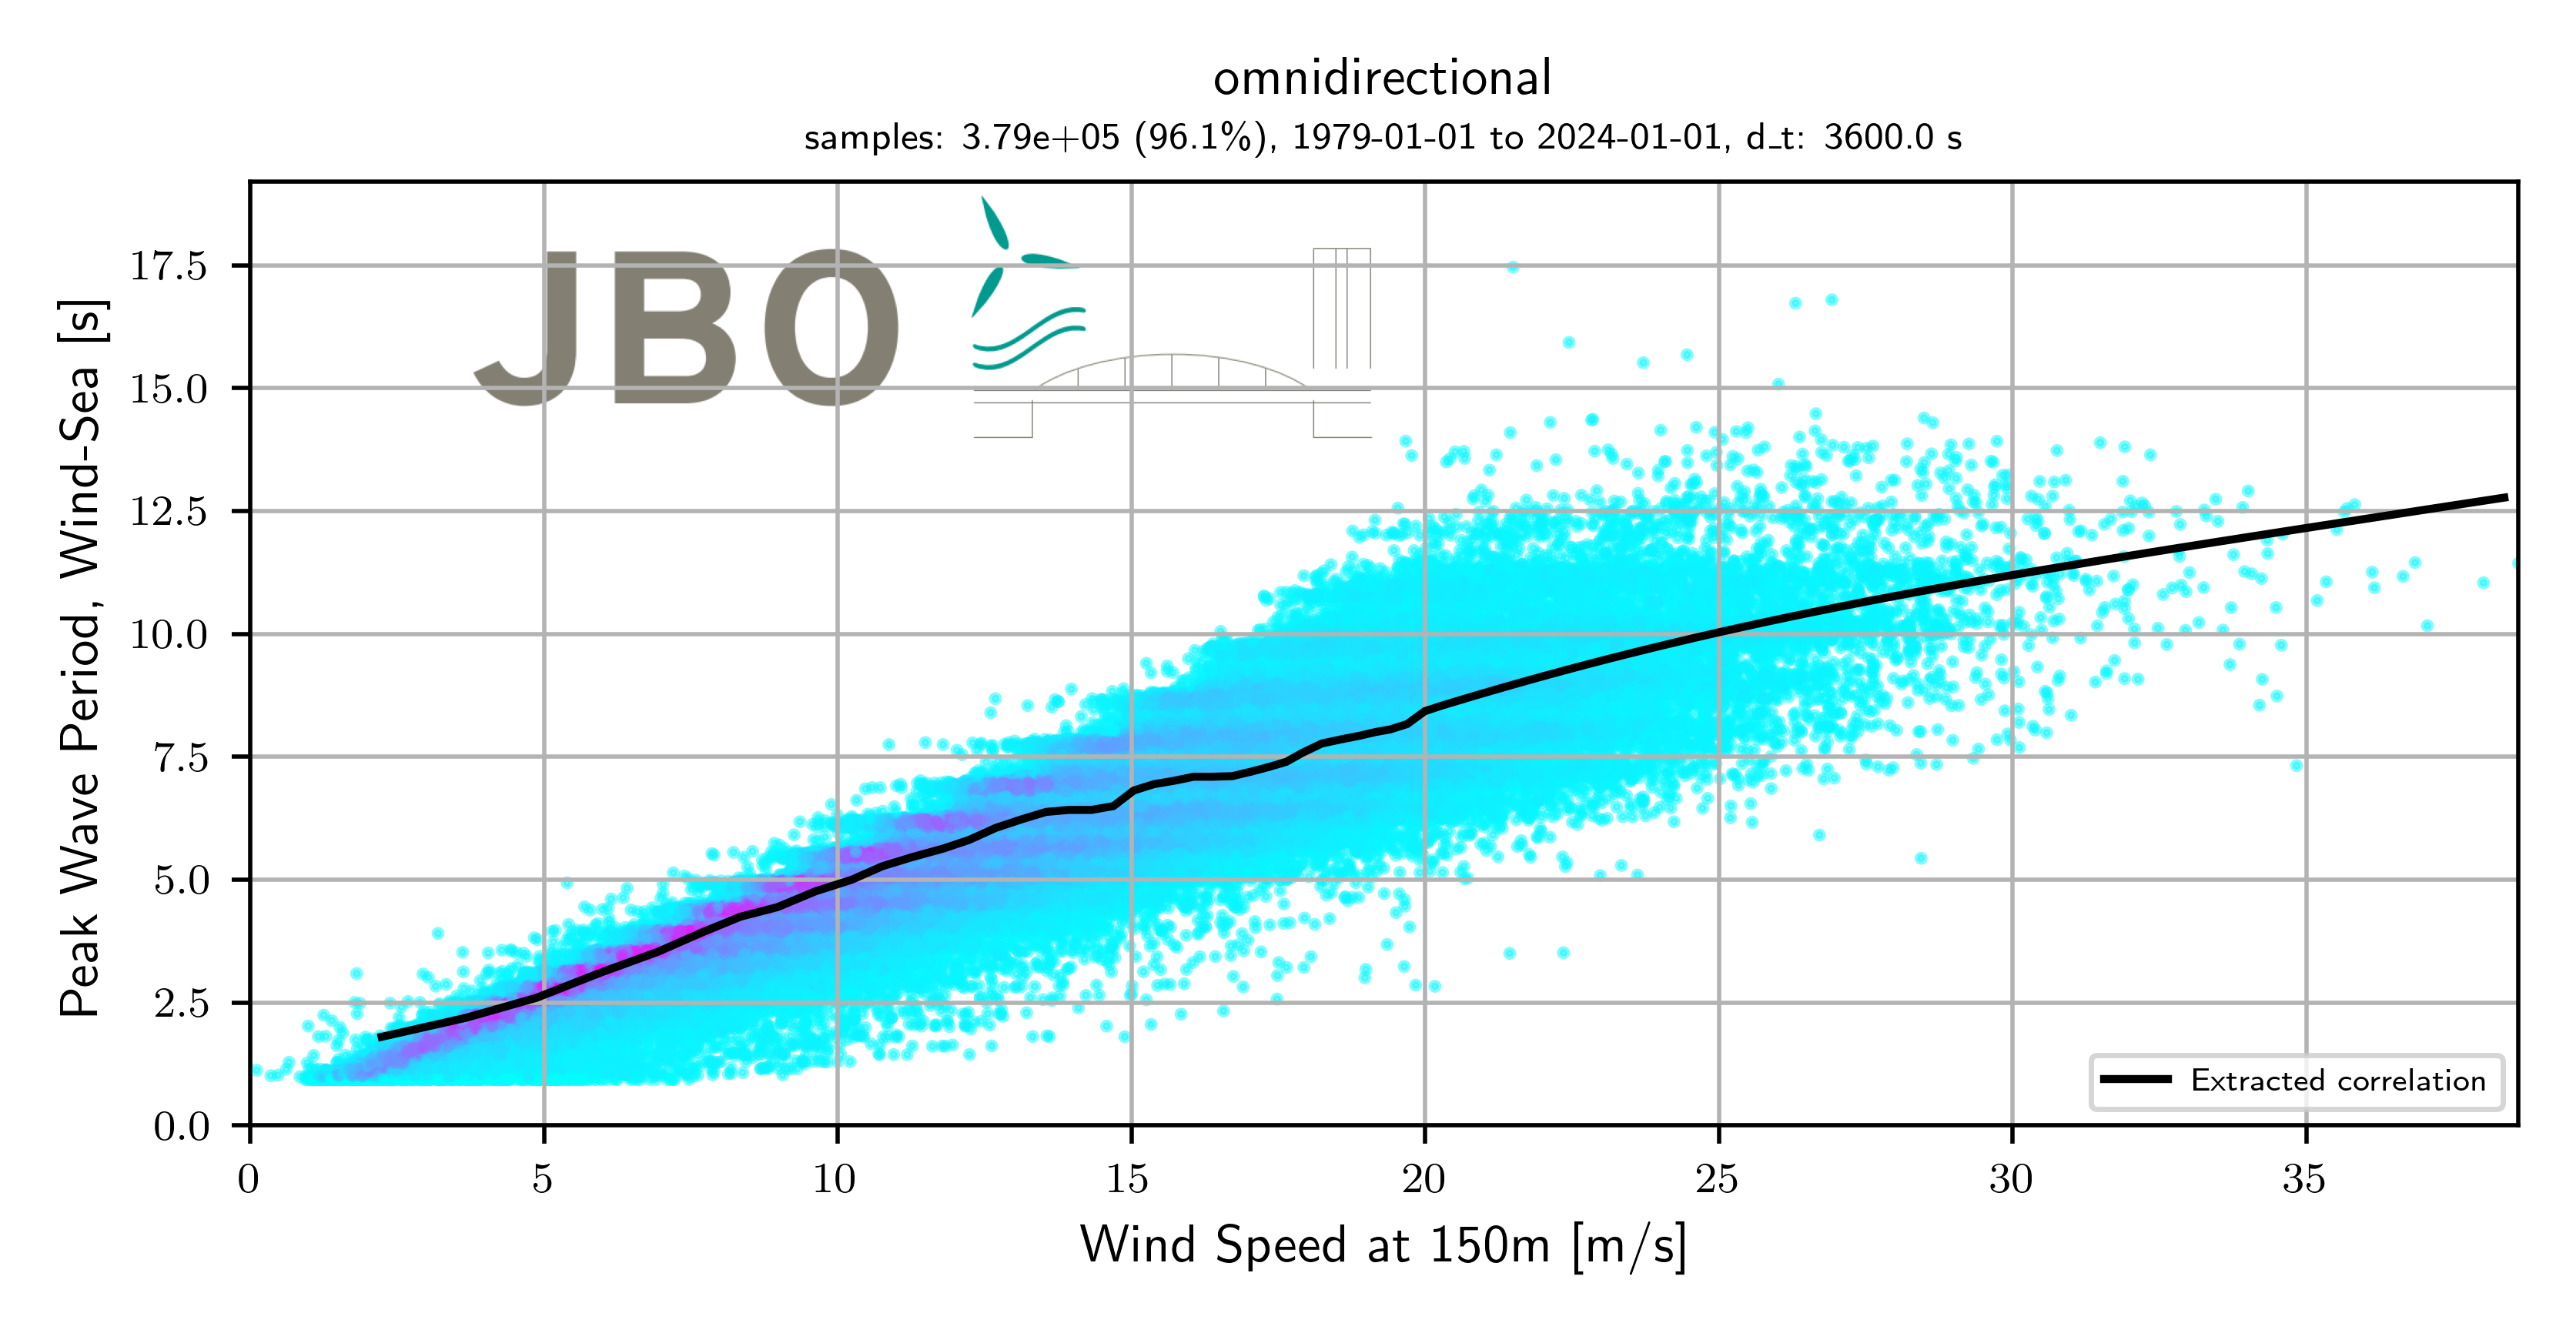
\includegraphics[width=1.0\textwidth]{C:/Users/aaron.lange/Desktop/Projekte/Hindcast_Tool/HindTool/example_output/VMTP_wind_page_3.png} 
 \caption{ VMTP-wind-page-3 } 
 \label{fig: VMTP_wind_page_3 } 
\end{figure}

\subsubsection{Summary tables of normal sea state conditions}
For the final condensation of the sea state-parameters the $H_s$ and $T_p$ values are determined using the $H_s(V_s)$ and $T_p(V_m)$ correlations. Therefore, the small-gridded functions are used to interpolate the data on the desired v_m- grid. The values are only calculated in the $v_m$ - range with data given. Bins inside the evaluated limits with zero occurrence probabilities are greyed out. The results are displayed in the tables (REF).

\begin{figure}[H] 
 \centering 
 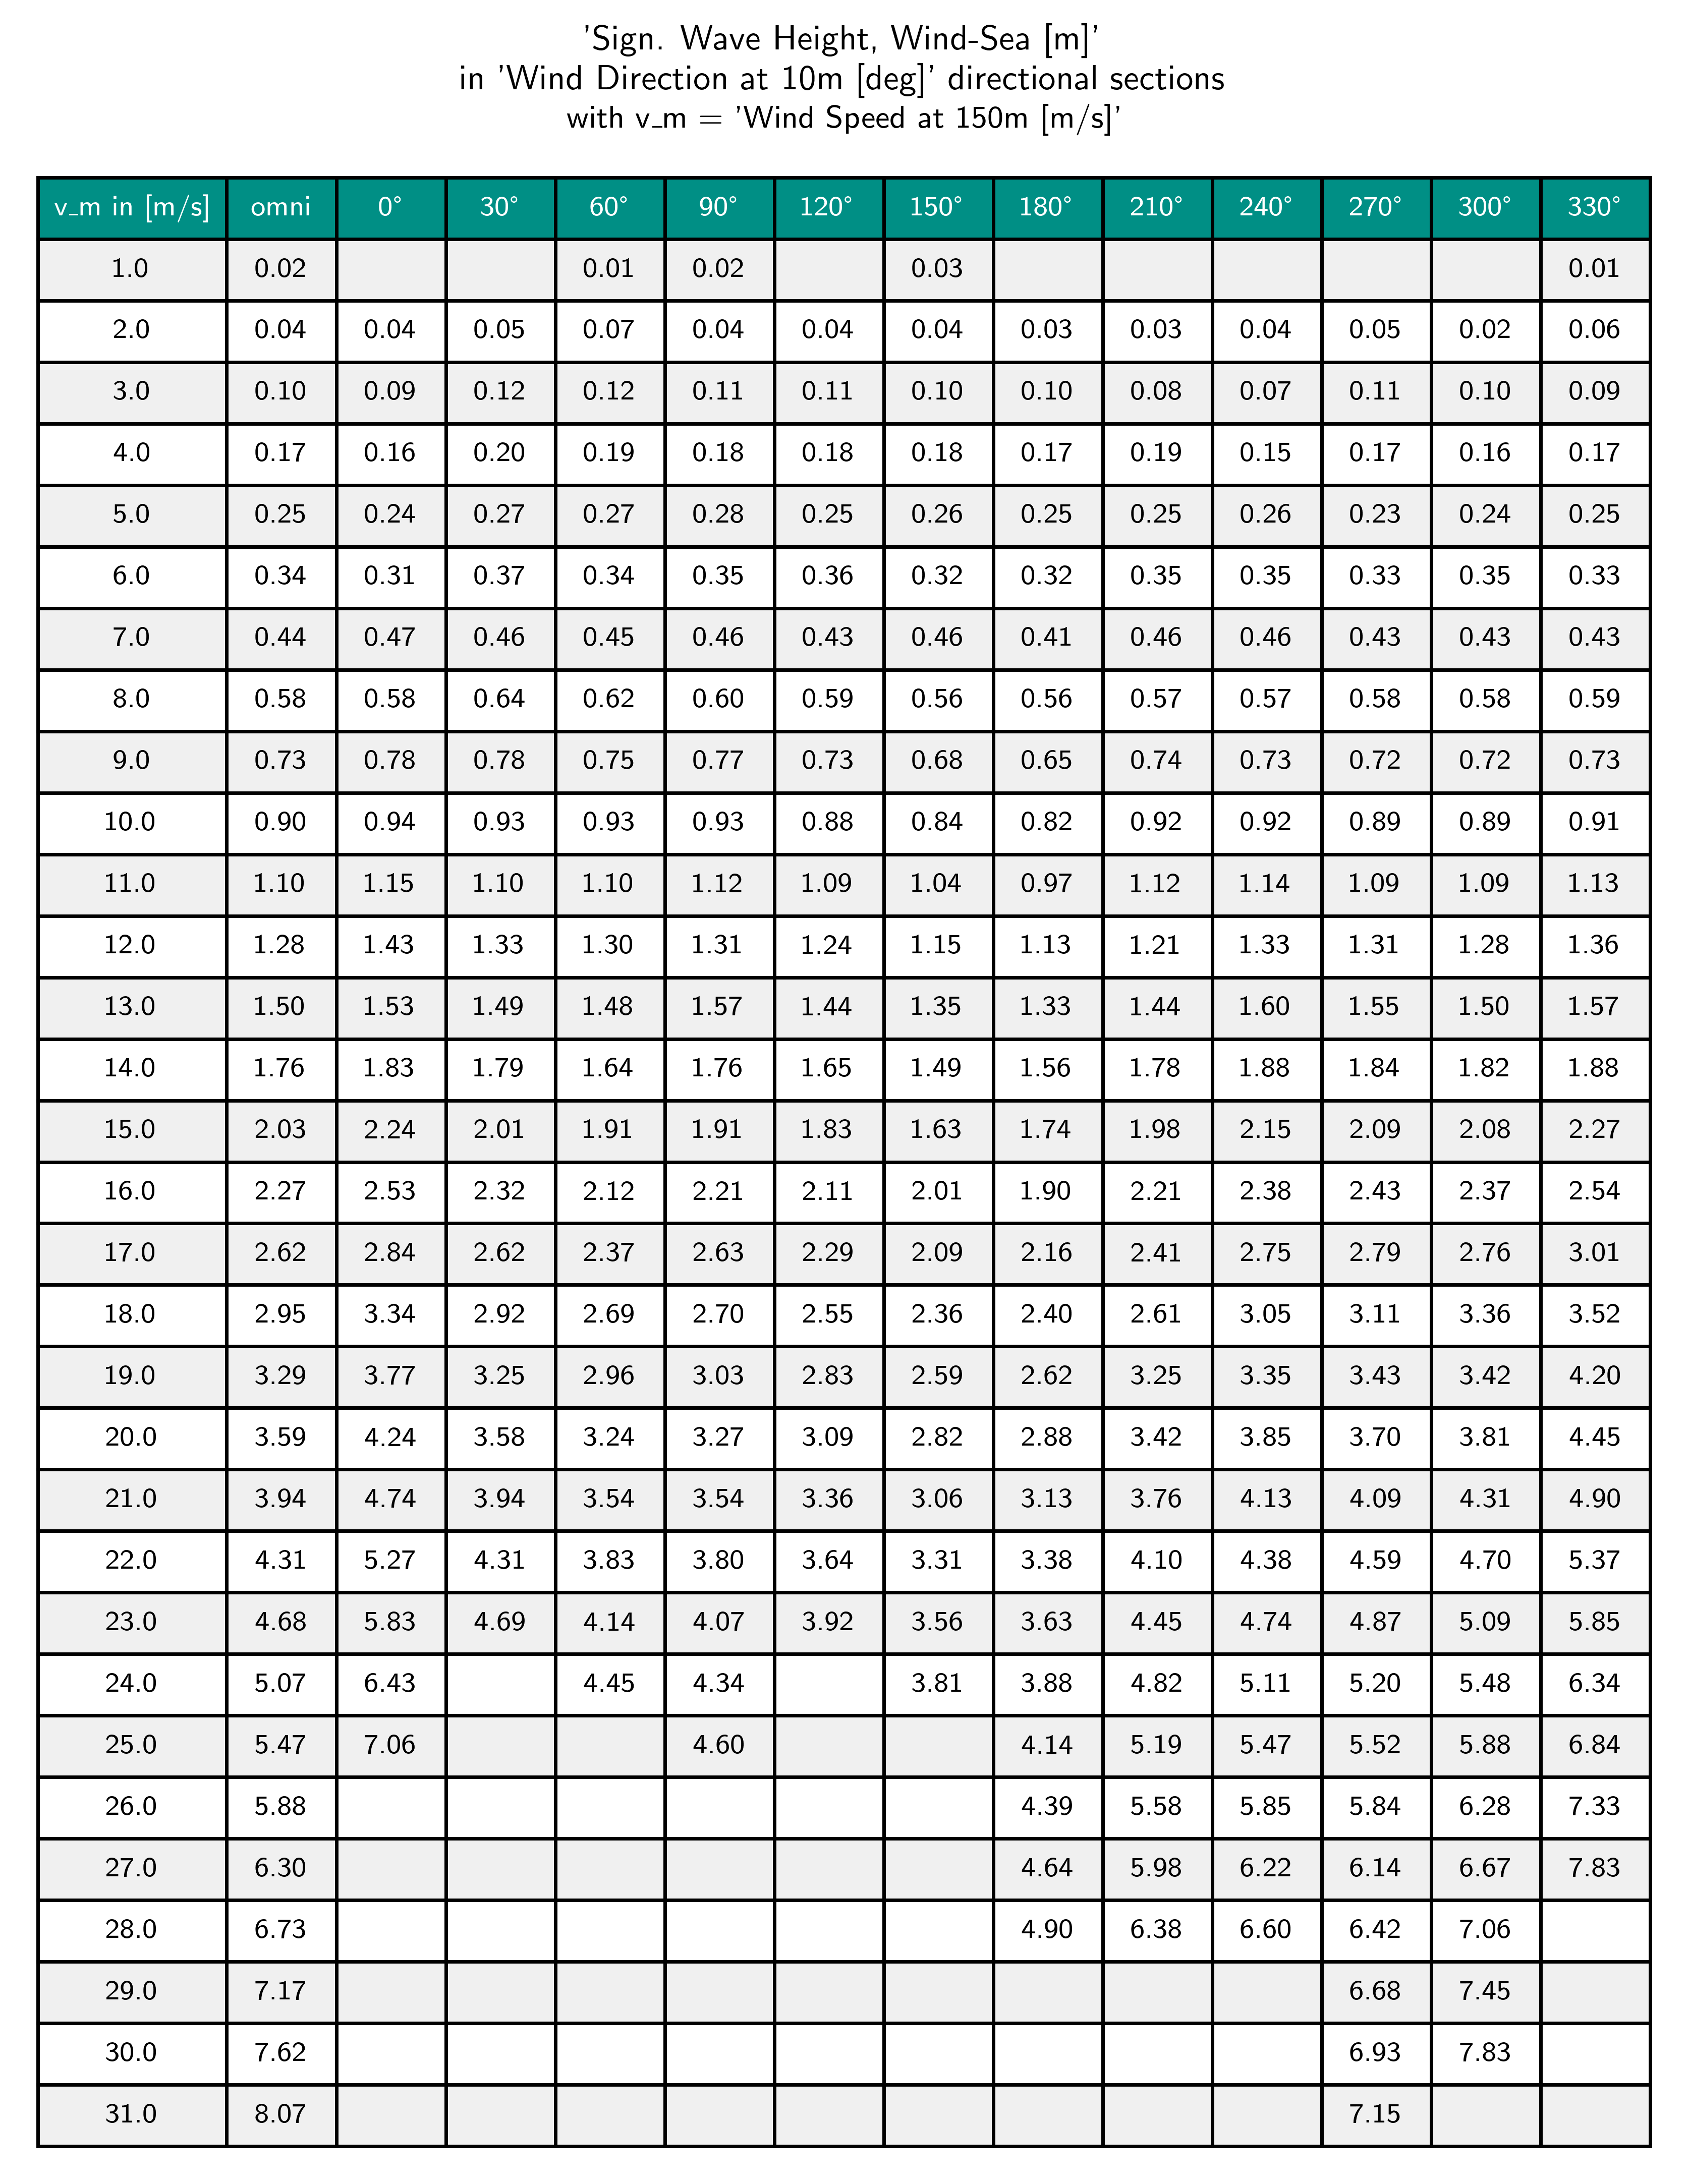
\includegraphics[width=1.0\textwidth ]{C:/Users/aaron.lange/Desktop/Projekte/Hindcast_Tool/HindTool/example_output/table_vmhs_wind_page_1.png} 
 \captionsetup{type=table} 
\caption{ table-vmhs-wind-page-1 } 
 \label{tab: table_vmhs_wind_page_1 } 
\end{figure}
\begin{figure}[H] 
 \centering 
 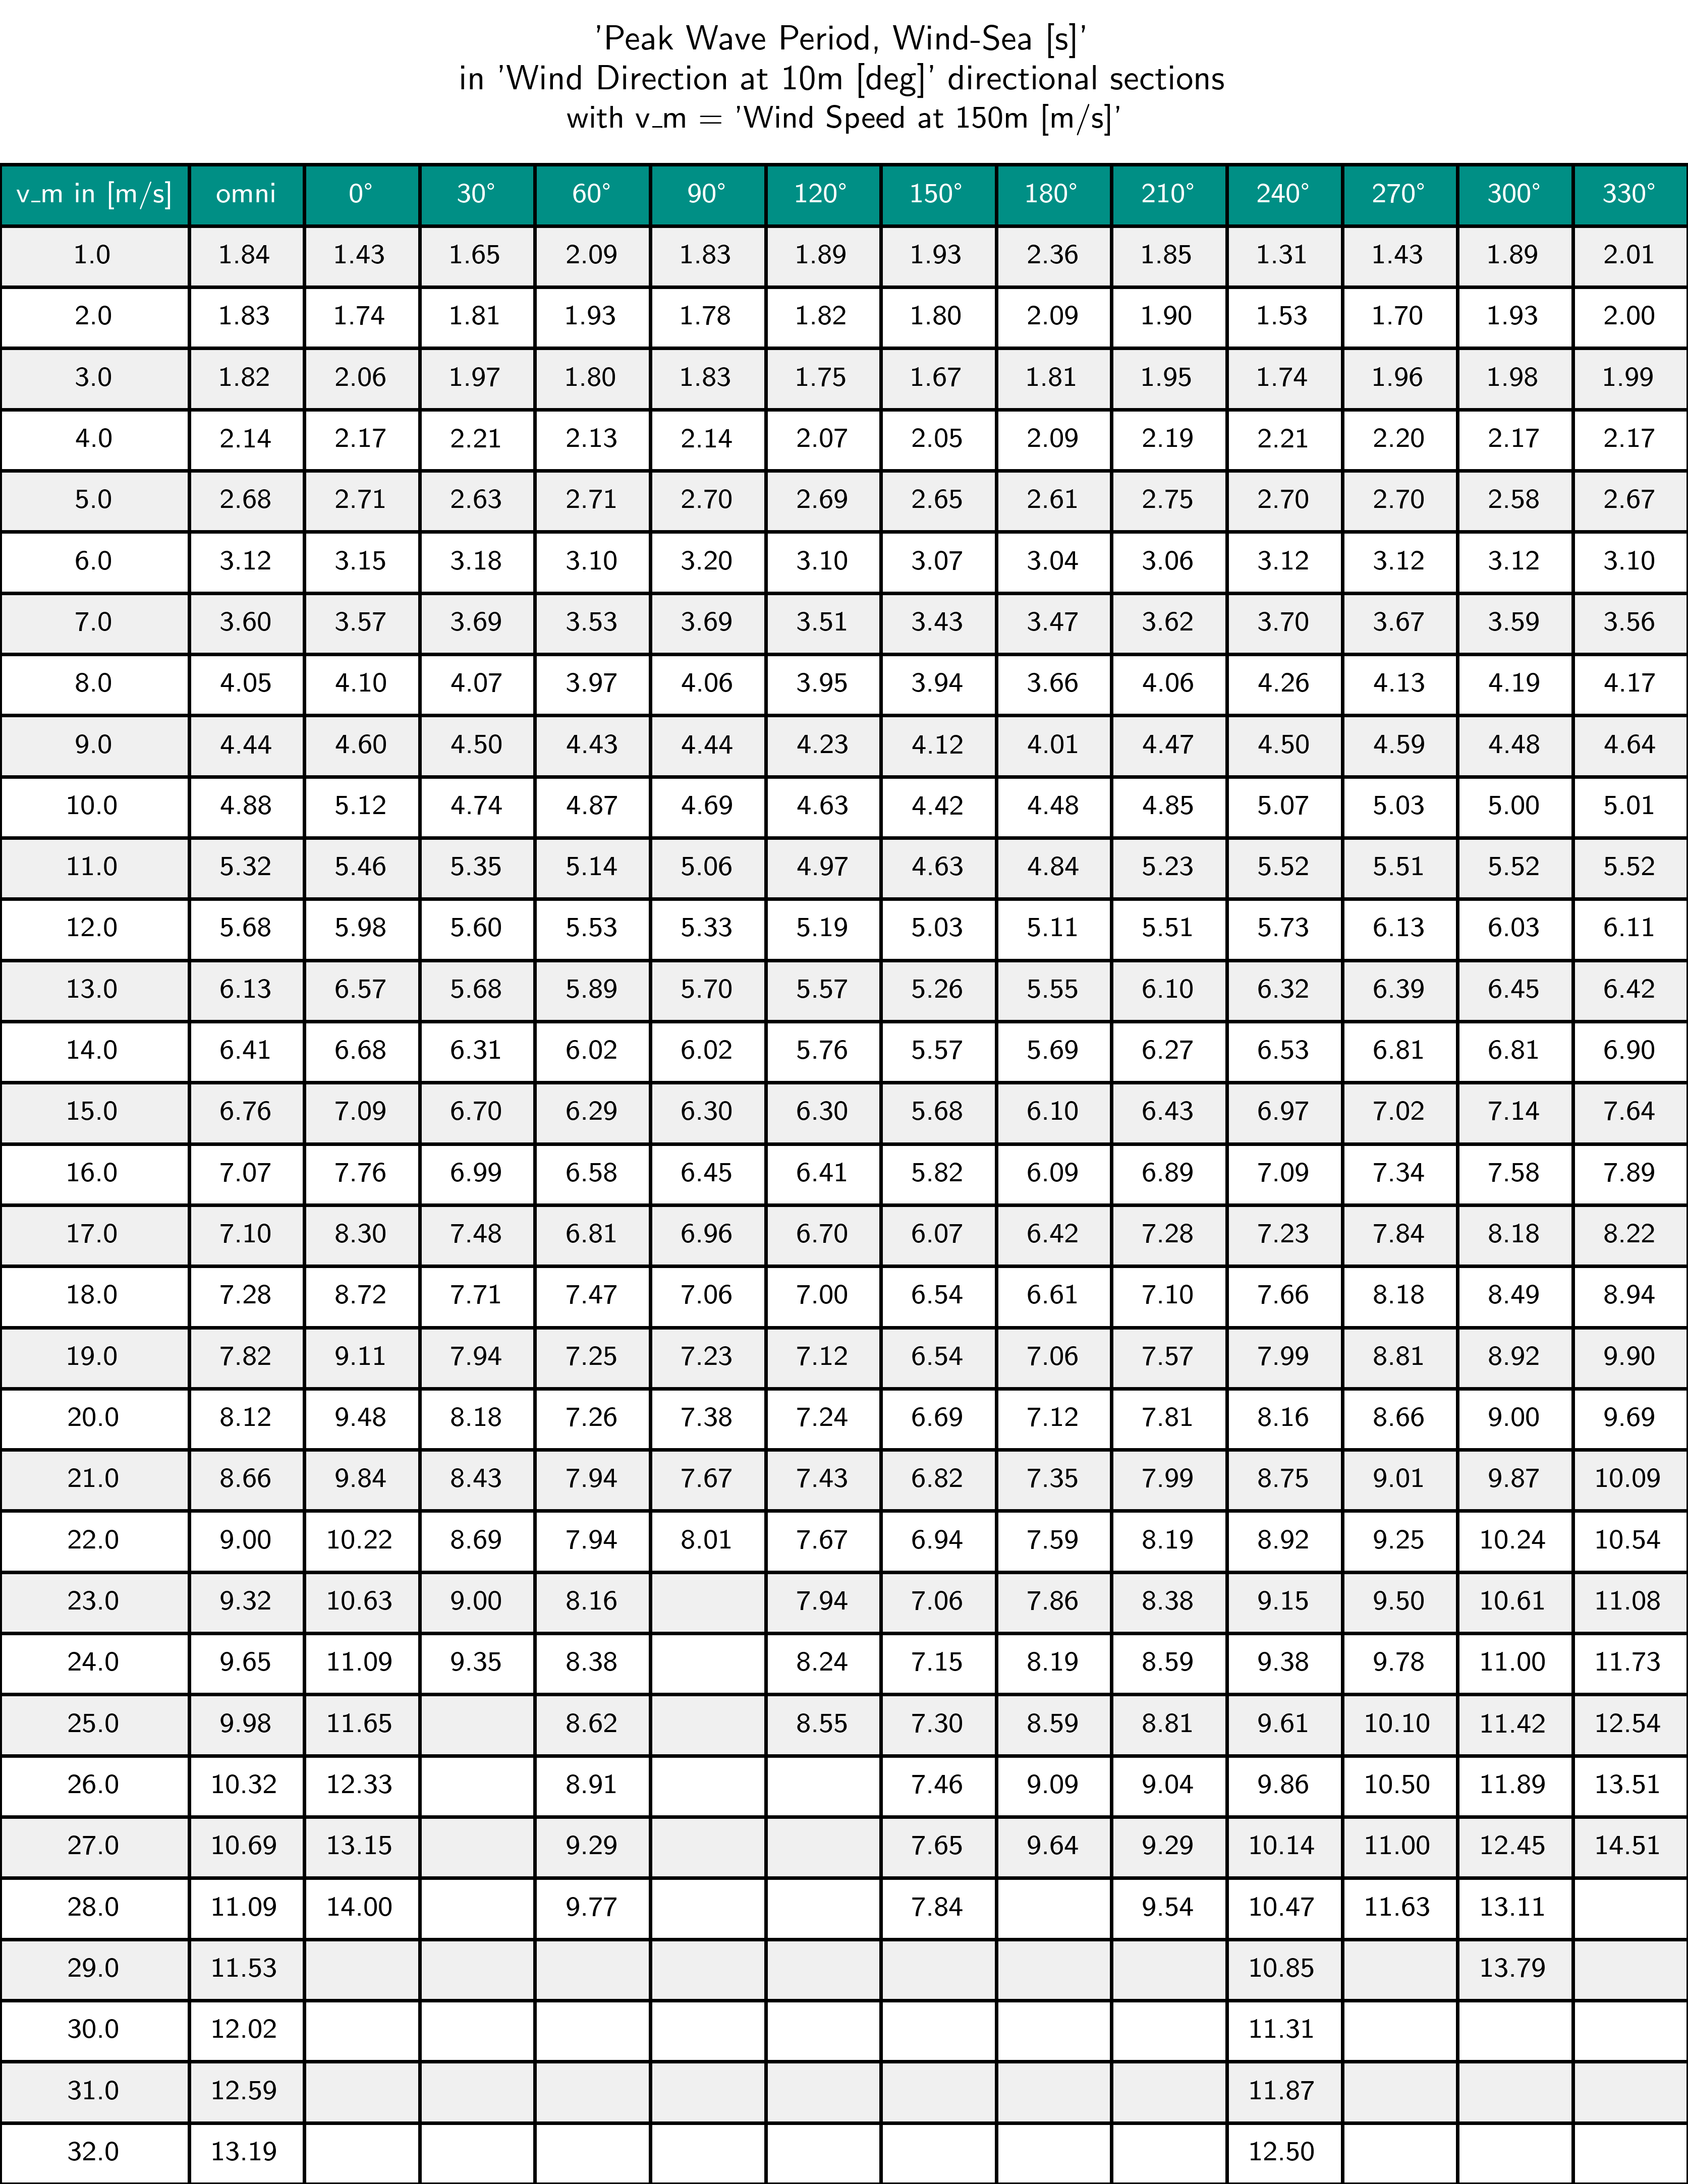
\includegraphics[width=1.0\textwidth ]{C:/Users/aaron.lange/Desktop/Projekte/Hindcast_Tool/HindTool/example_output/table_vmtp_wind_page_1.png} 
 \captionsetup{type=table} 
\caption{ table-vmtp-wind-page-1 } 
 \label{tab: table_vmtp_wind_page_1 } 
\end{figure}
\begin{figure}[H] 
 \centering 
 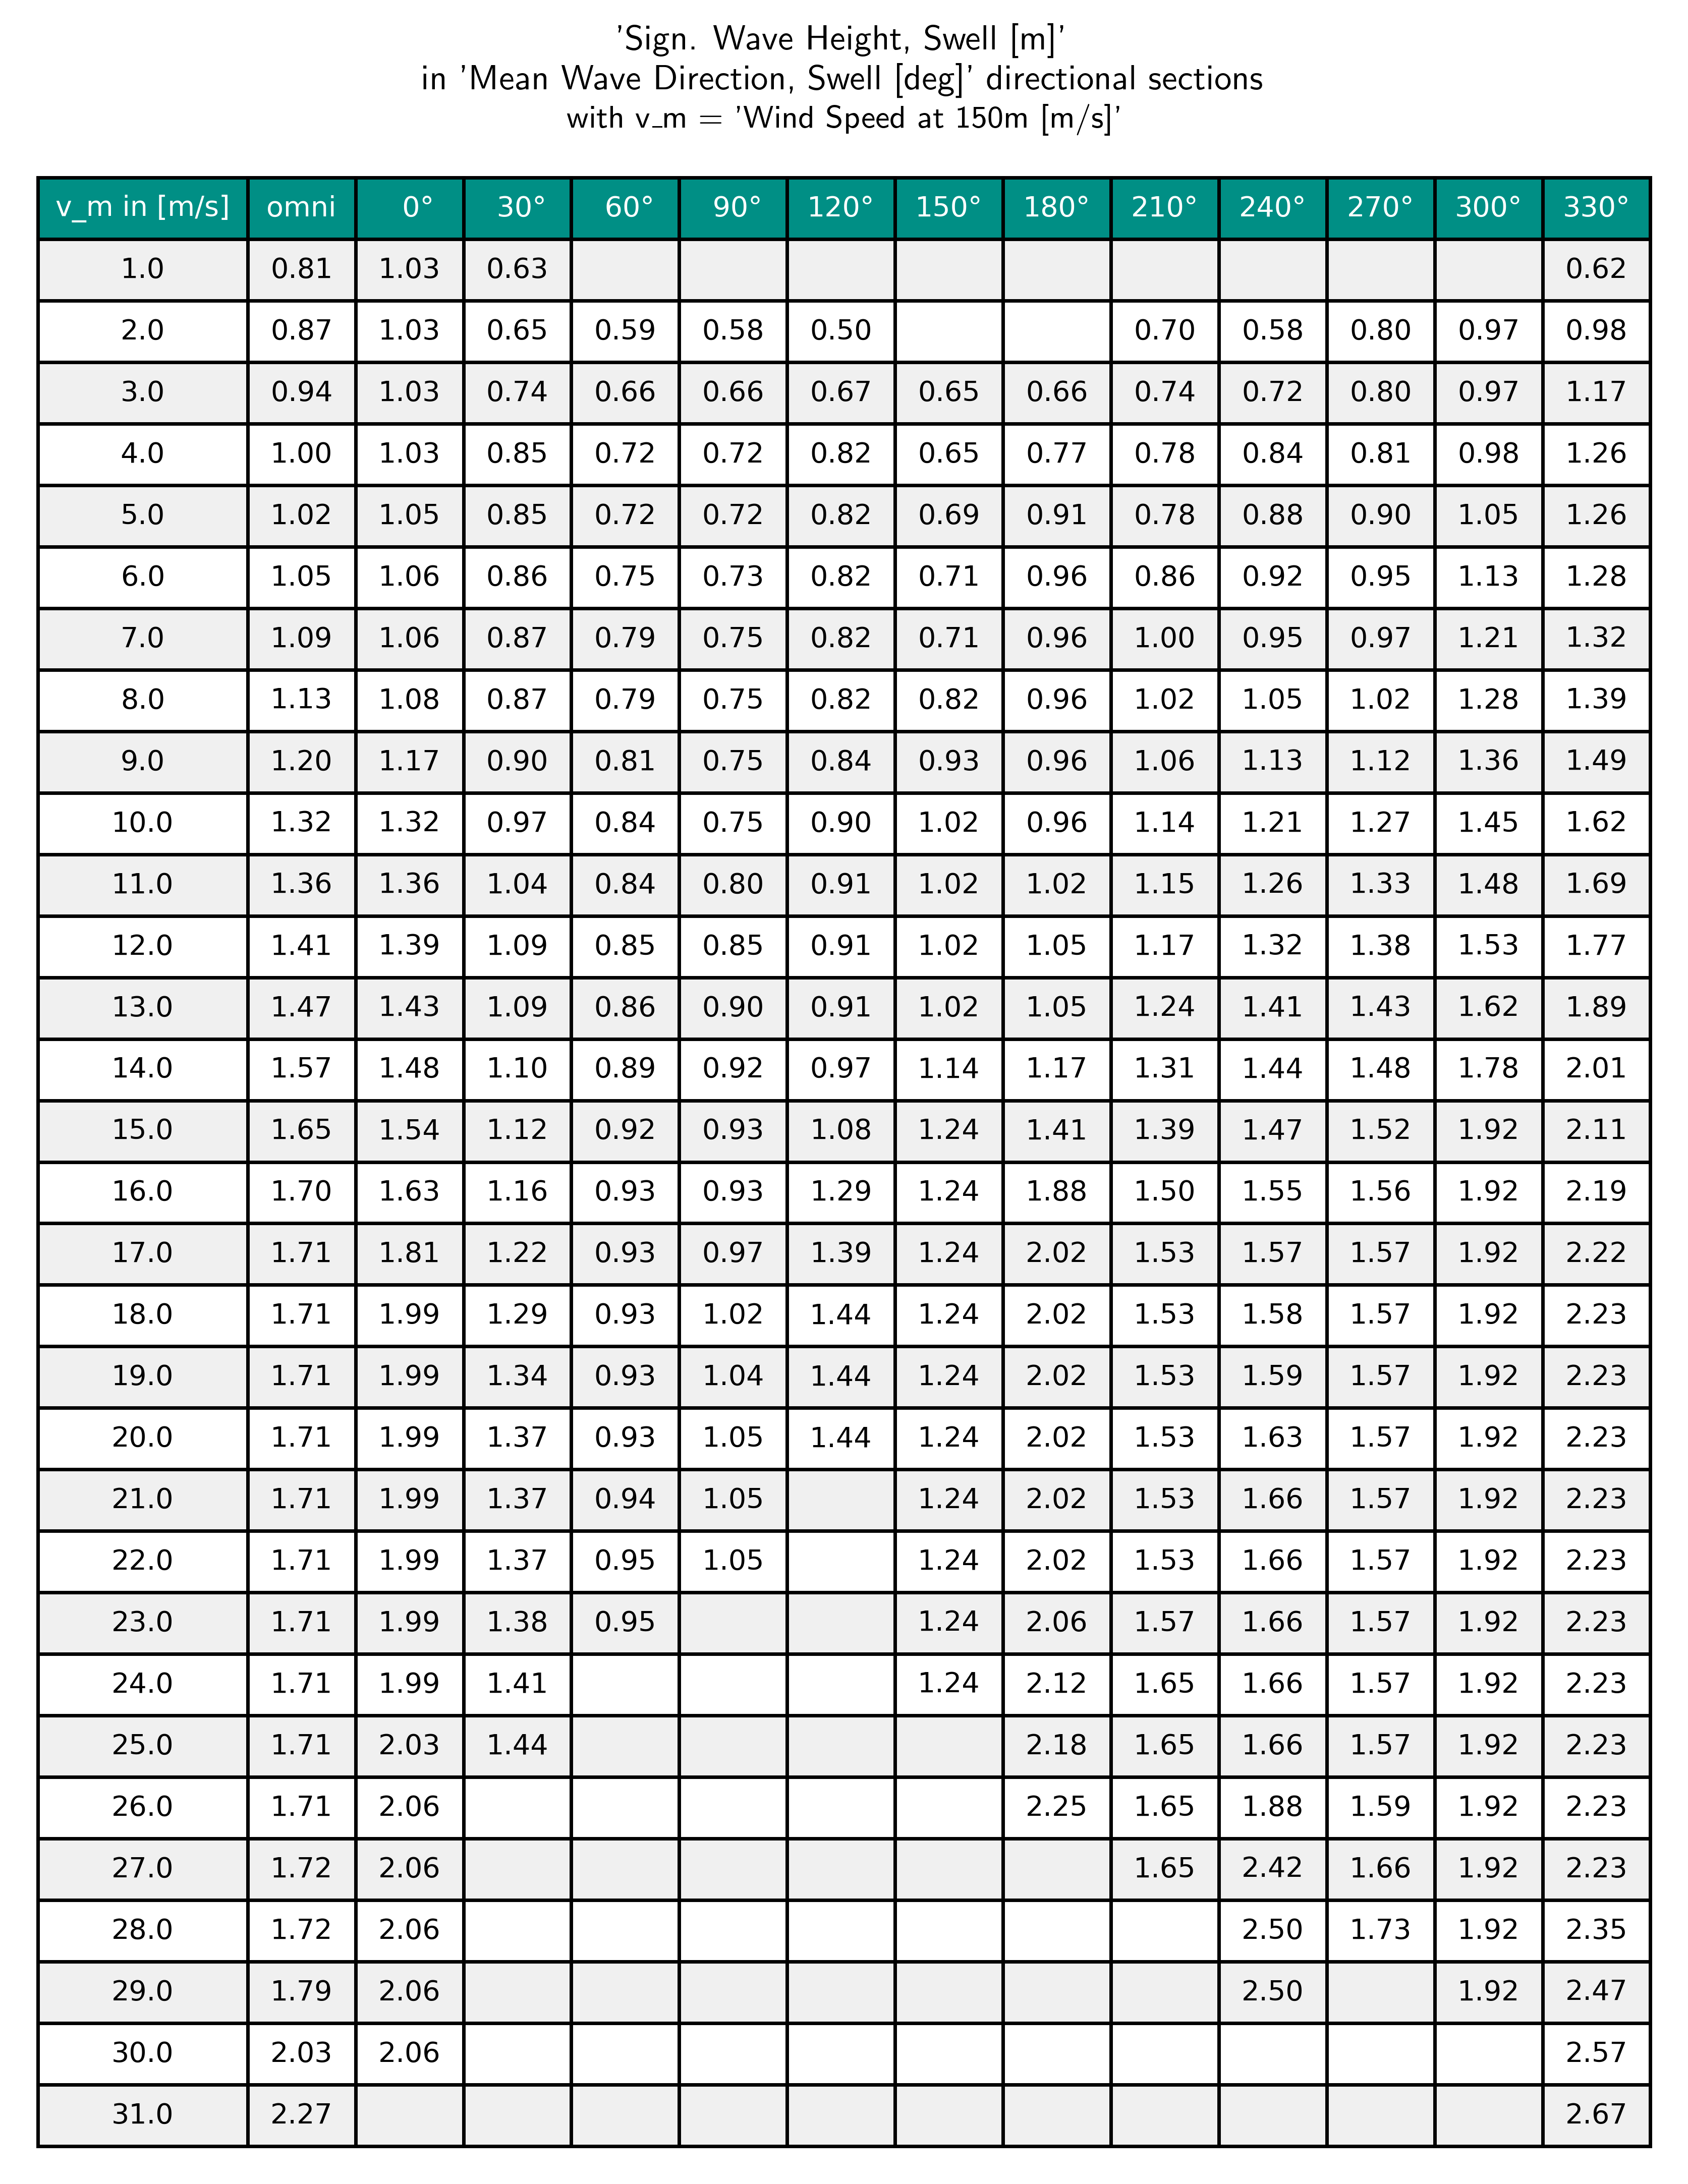
\includegraphics[width=1.0\textwidth ]{C:/Users/aaron.lange/Desktop/Projekte/Hindcast_Tool/HindTool/example_output/table_vmhs_swell_page_1.png} 
 \captionsetup{type=table} 
\caption{ table-vmhs-swell-page-1 } 
 \label{tab: table_vmhs_swell_page_1 } 
\end{figure}
\begin{figure}[H] 
 \centering 
 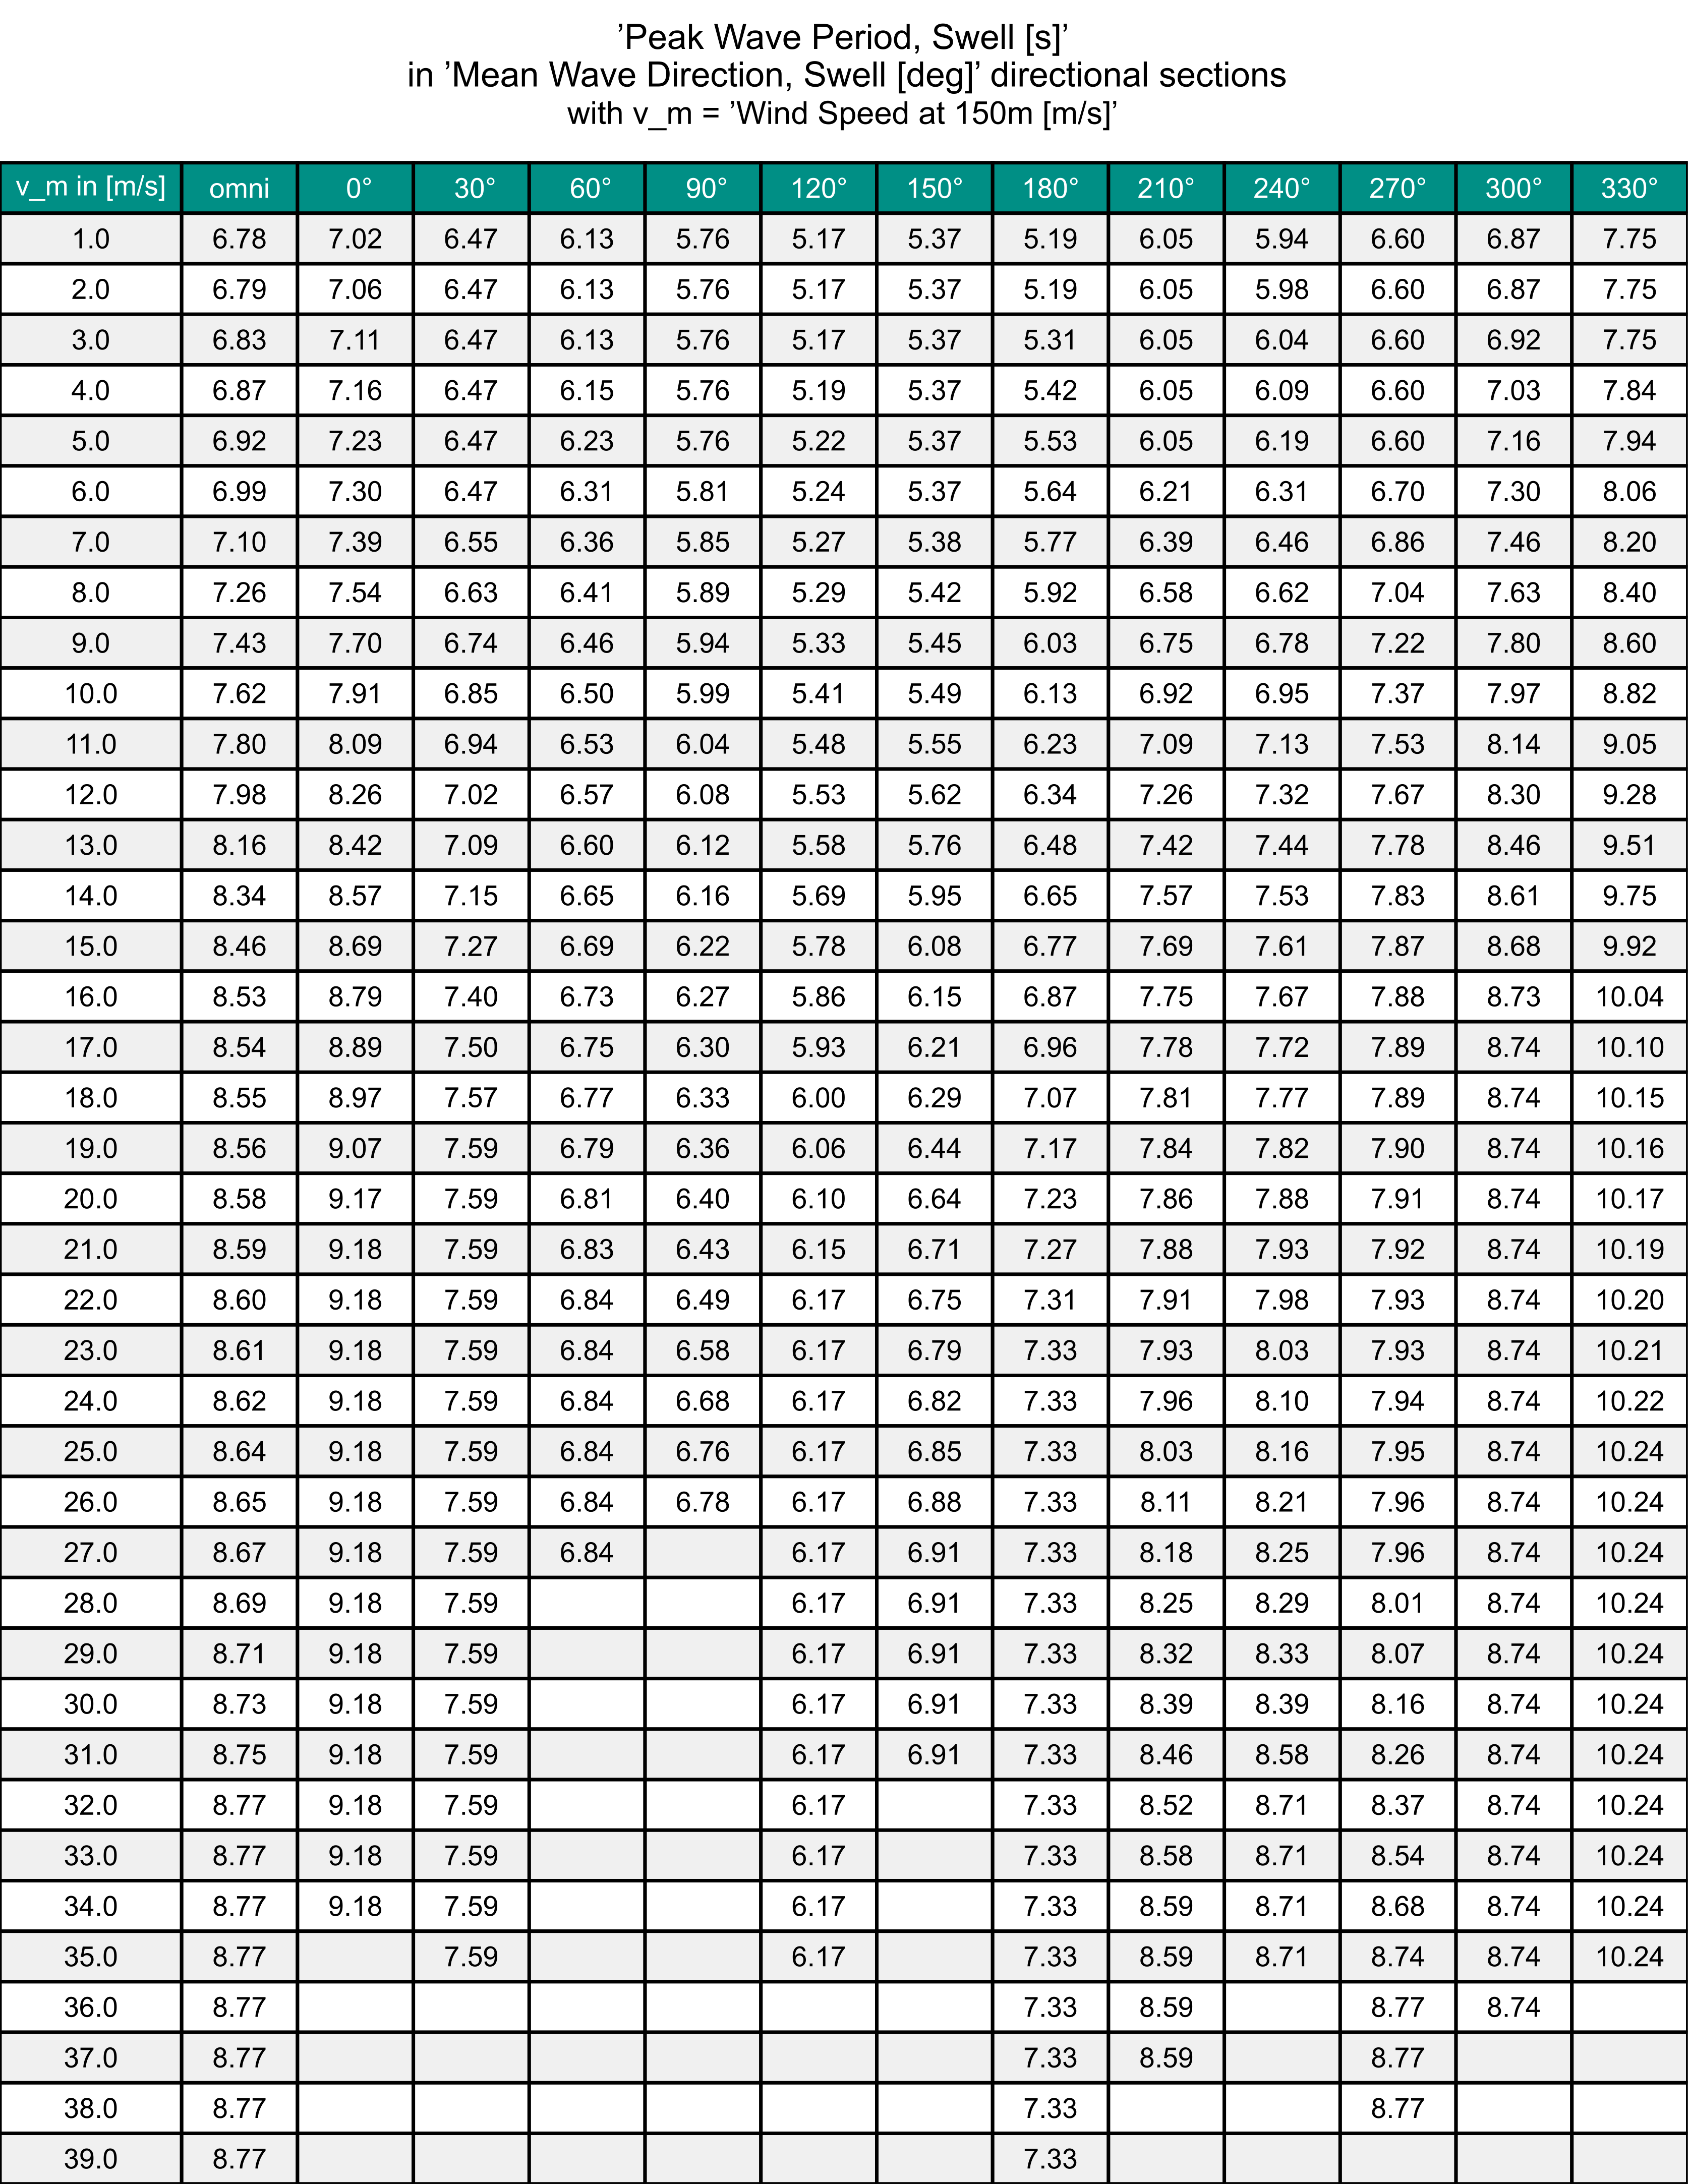
\includegraphics[width=1.0\textwidth ]{C:/Users/aaron.lange/Desktop/Projekte/Hindcast_Tool/HindTool/example_output/table_vmtp_swell_page_1.png} 
 \captionsetup{type=table} 
\caption{ table-vmtp-swell-page-1 } 
 \label{tab: table_vmtp_swell_page_1 } 
\end{figure}

\subsection{Proof of condensation method}
The proof of the condensation method for normal sea state parameter is provided in this section in detail. A reference structural FE model of the intended WTG and foundation configuration has been set up for this purpose. Using a frequency domain approach, damage equivalent loads of the bending moment at decisive elevations are calculated for each individual sea state sample in the data set.
\\
Damage equivalent loads are applied to equate the fatigue damage represented by rainflow cycle counted data to that caused by a single stress range repeating at a single frequency. The method is based on the Miner's rule. The damage equivalent load is given by the following formula:

$$
L_{N}(m)=\sqrt[m]{\frac{\sum_{i=1}^{k} L_{i}^{m} n_{i}}{N}}
$$

where:
\quad $ L_{N} $ \quad is the equivalent stress for $N$ cycles in the specified design life\\
\quad $ L_{i} $ \quad is the stress range bin $i$\\
\quad $ n_{i} $ \quad is the number of rain flow cycles at stress range bin $i$\\
\quad $ k $ \quad  is the number of bins\\
\quad $ m $ \quad  is the negative inverse of the slope on the material's Woehler curve (m is also referred to as the S-N curve slope) \\
\quad $ N $ \quad  is the reference number of cycle repetitions (1E7 in this case) \\

The stress, $L_{i}$ depends upon the geometry of the structure. It is assumed that stress is proportional to load, therefore it is acceptable to use load instead of stress in the above equation.
\\
An overview of the load analysis results for an exemplary bending moment in frequency domain for the reference structure ( $1^{\text {st }} \mathrm{EF}=f_{0}$ ) is provided below.\\

\begin{figure}[H] 
 \centering 
 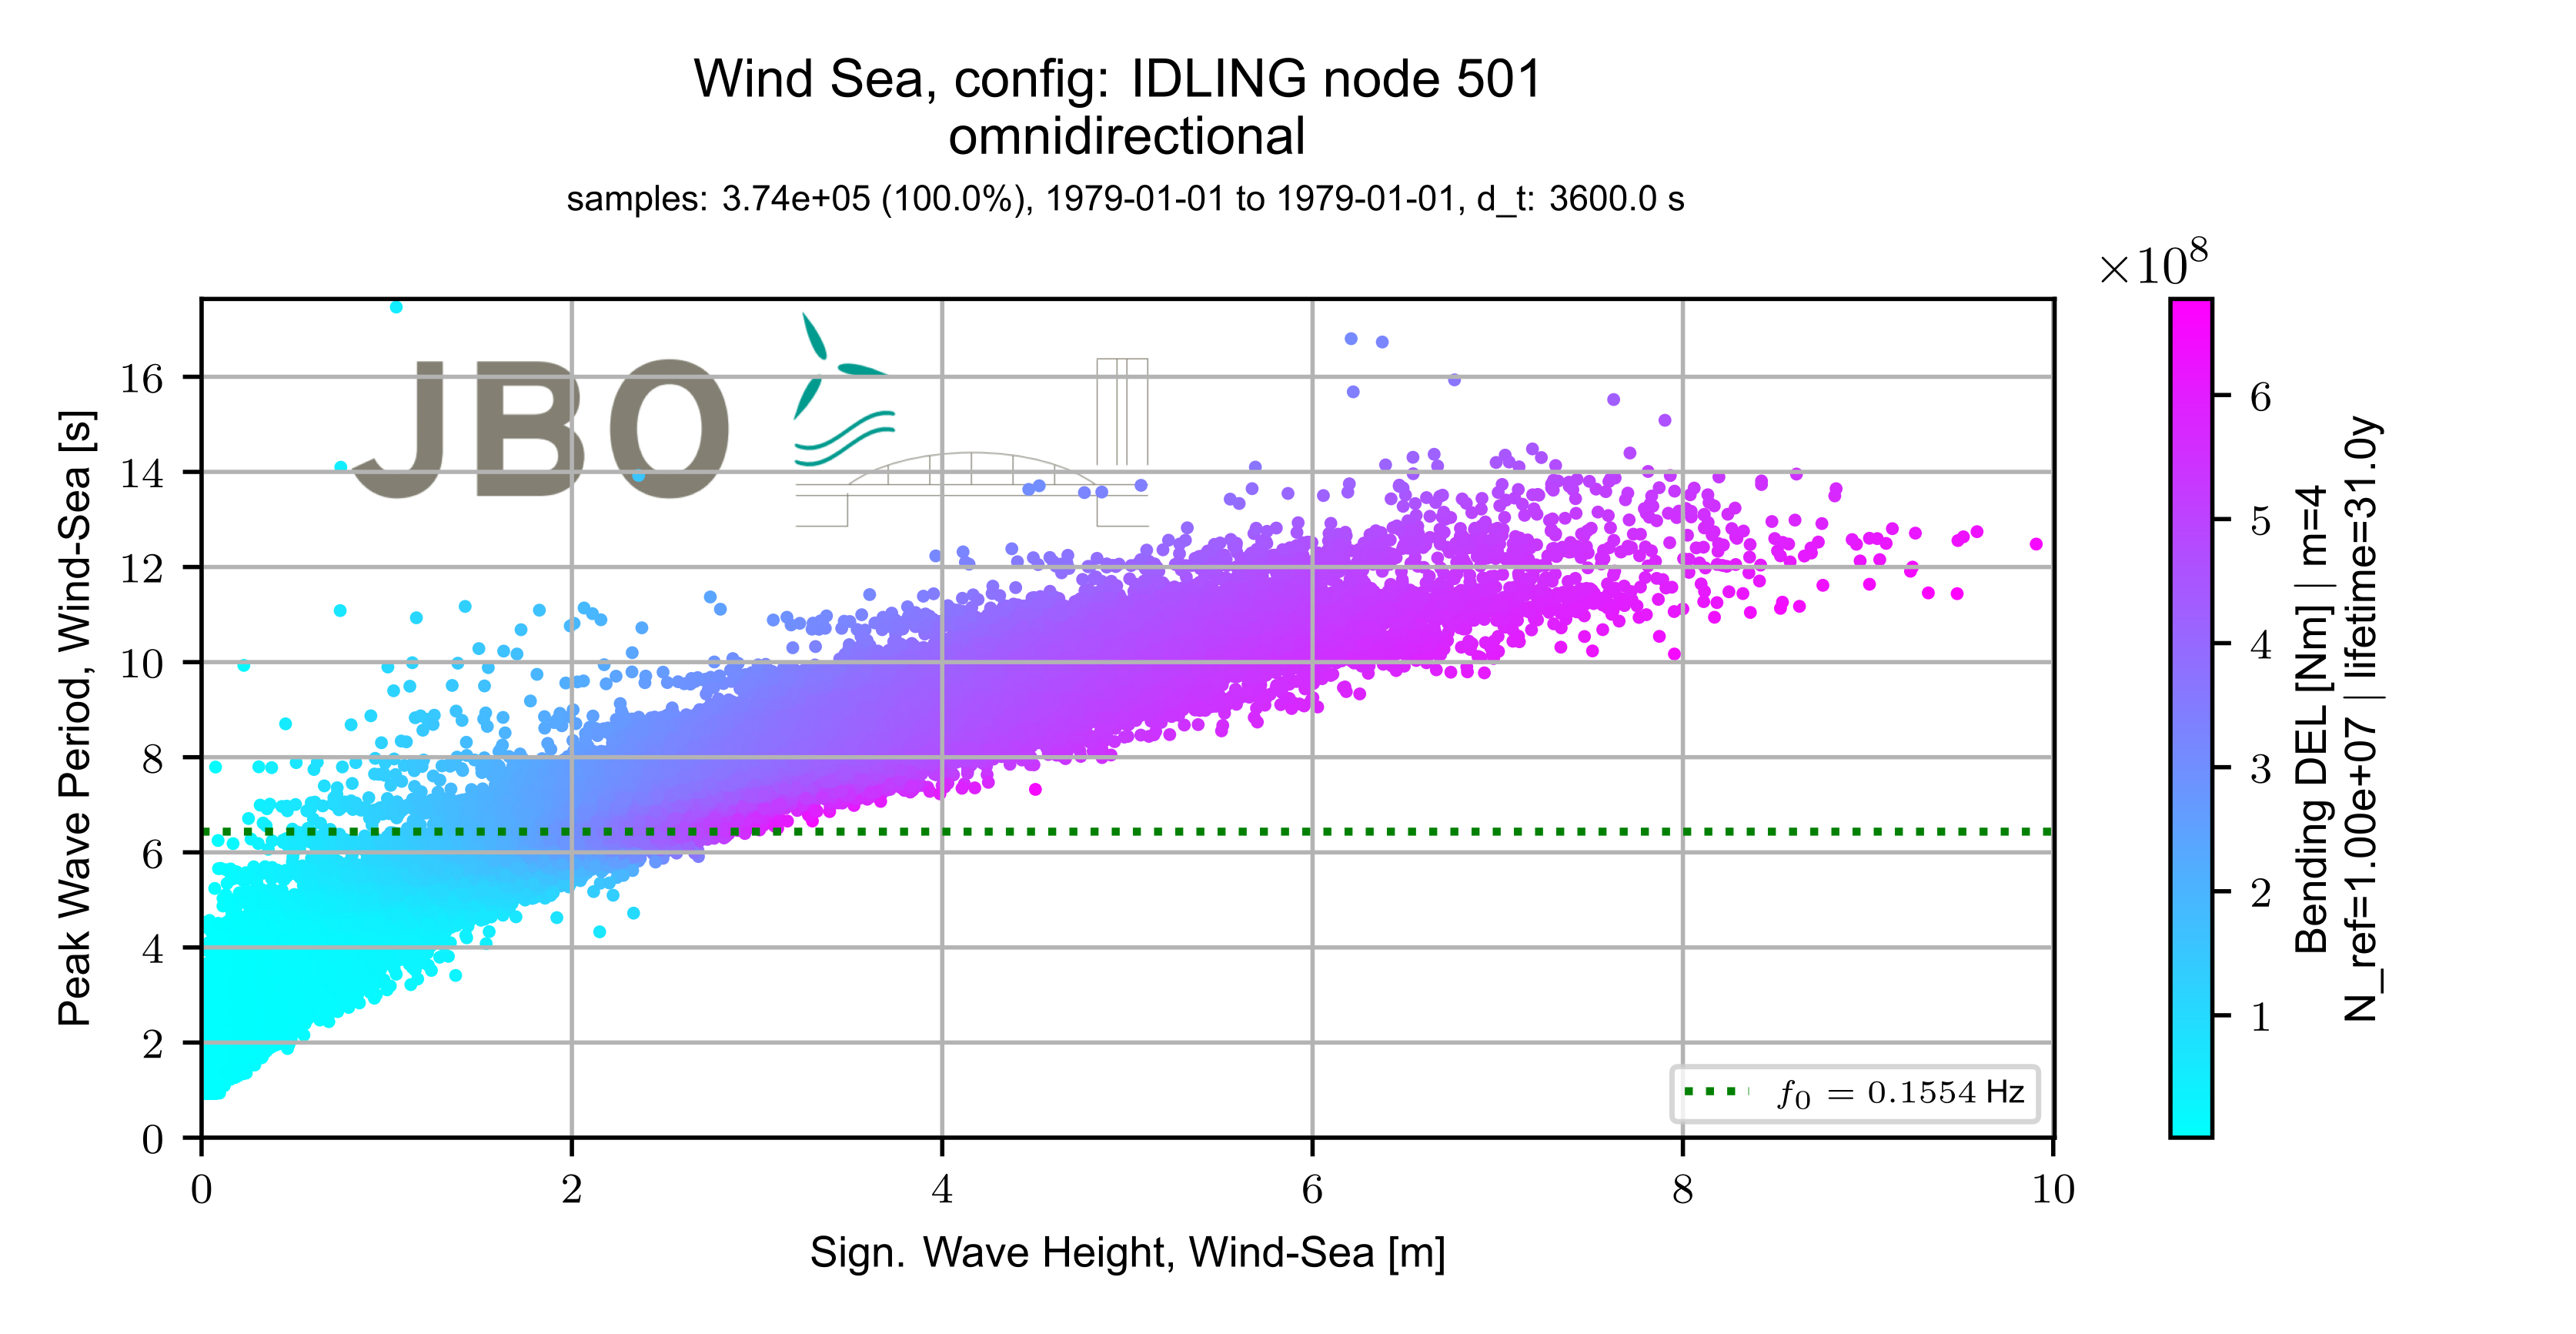
\includegraphics[width=1.0\textwidth]{C:/Users/aaron.lange/Desktop/Projekte/Hindcast_Tool/HindTool/example_output/Valid_scatter_wind_page_3.png} 
 \caption{ Valid-scatter-wind-page-3 } 
 \label{fig: Valid_scatter_wind_page_3 } 
\end{figure}
\begin{figure}[H] 
 \centering 
 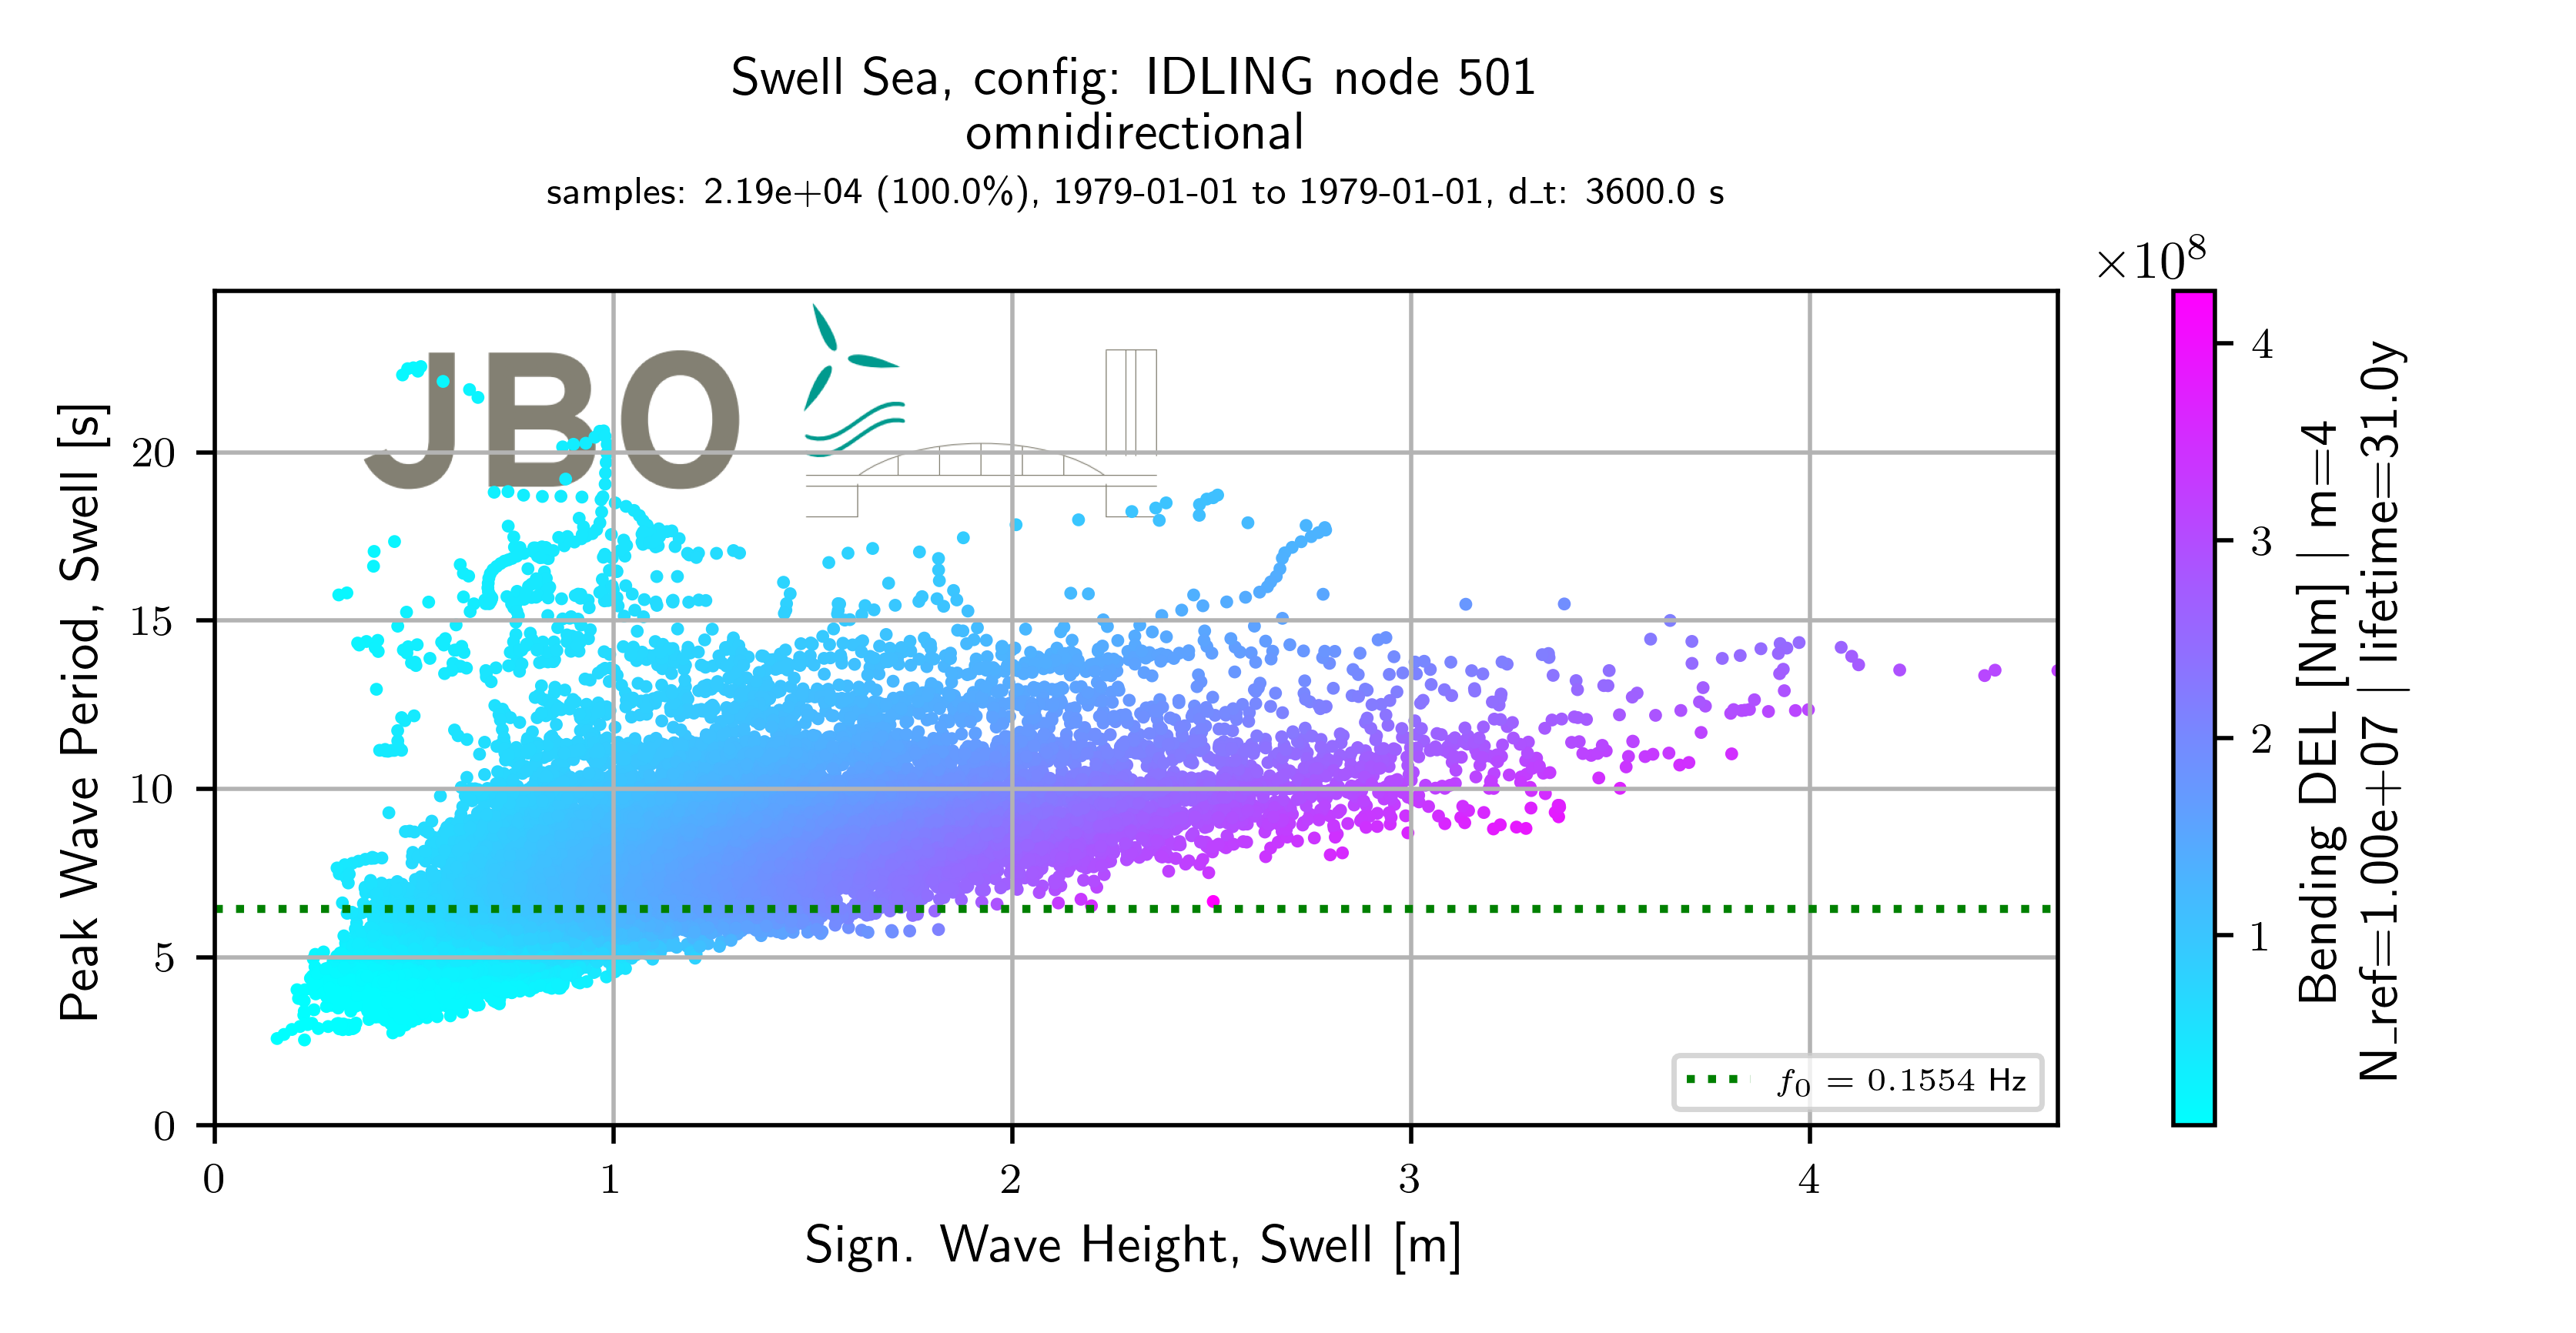
\includegraphics[width=1.0\textwidth]{C:/Users/aaron.lange/Desktop/Projekte/Hindcast_Tool/HindTool/example_output/Valid_scatter_swell_page_3.png} 
 \caption{ Valid-scatter-swell-page-3 } 
 \label{fig: Valid_scatter_swell_page_3 } 
\end{figure}


In the validation, DELs for idling conditions (very low aerodynamic damping contribution) and production conditions (incl. significant aerodynamic damping contribution) are determined for the condensed sea state data sets and compared against the full scatter data sets. This is performed for omnidirectional and directional sets, based on the wind or swell direction. Occurrence probabilities are evaluated from the associated wind speed sensor. Damping from soil, material, hydro and radiation as well as the tower damper are included in the analysis.
\\
Figure 4-10Figure 4-11 and Figure 4-11Figure 4-12 below show:
\begin{itemize}
	\item The total condensed DEL vs. the full scatter (hindcast) DEL (text box top right)
	\item Wind speed dependent comparison of condensed and full scatter (hindcast) DEL
	\item The histogram of the underlying datapoints relative to the wind speed
	\item Number of data samples considered (legend at top)
\end{itemize}

A 100\% fit is always strived, however due to the nature of the joint occurrences of significant wave height and peak period this is not realistic. The chosen quantiles as described in section 4.7 .3 can be modified to achieve an optimized fit or a correction factor on the averaged values can be applied, see Table 4-1. The comparison between the condensed swell and the hindcast DEL typically shows different behaviors. This discrepancy is due to the fact that swell is defined by distant weather events and is therefore only low correlated to the local wind speed (as can be seen in Figure 4-4Figure 4-5 and Figure 4-6Figure 4-7). However, the parameters of the condensation method are adjusted to ensure that the overall DELs are at a similar load level.\\


\begin{figure}[H] 
 \centering 
 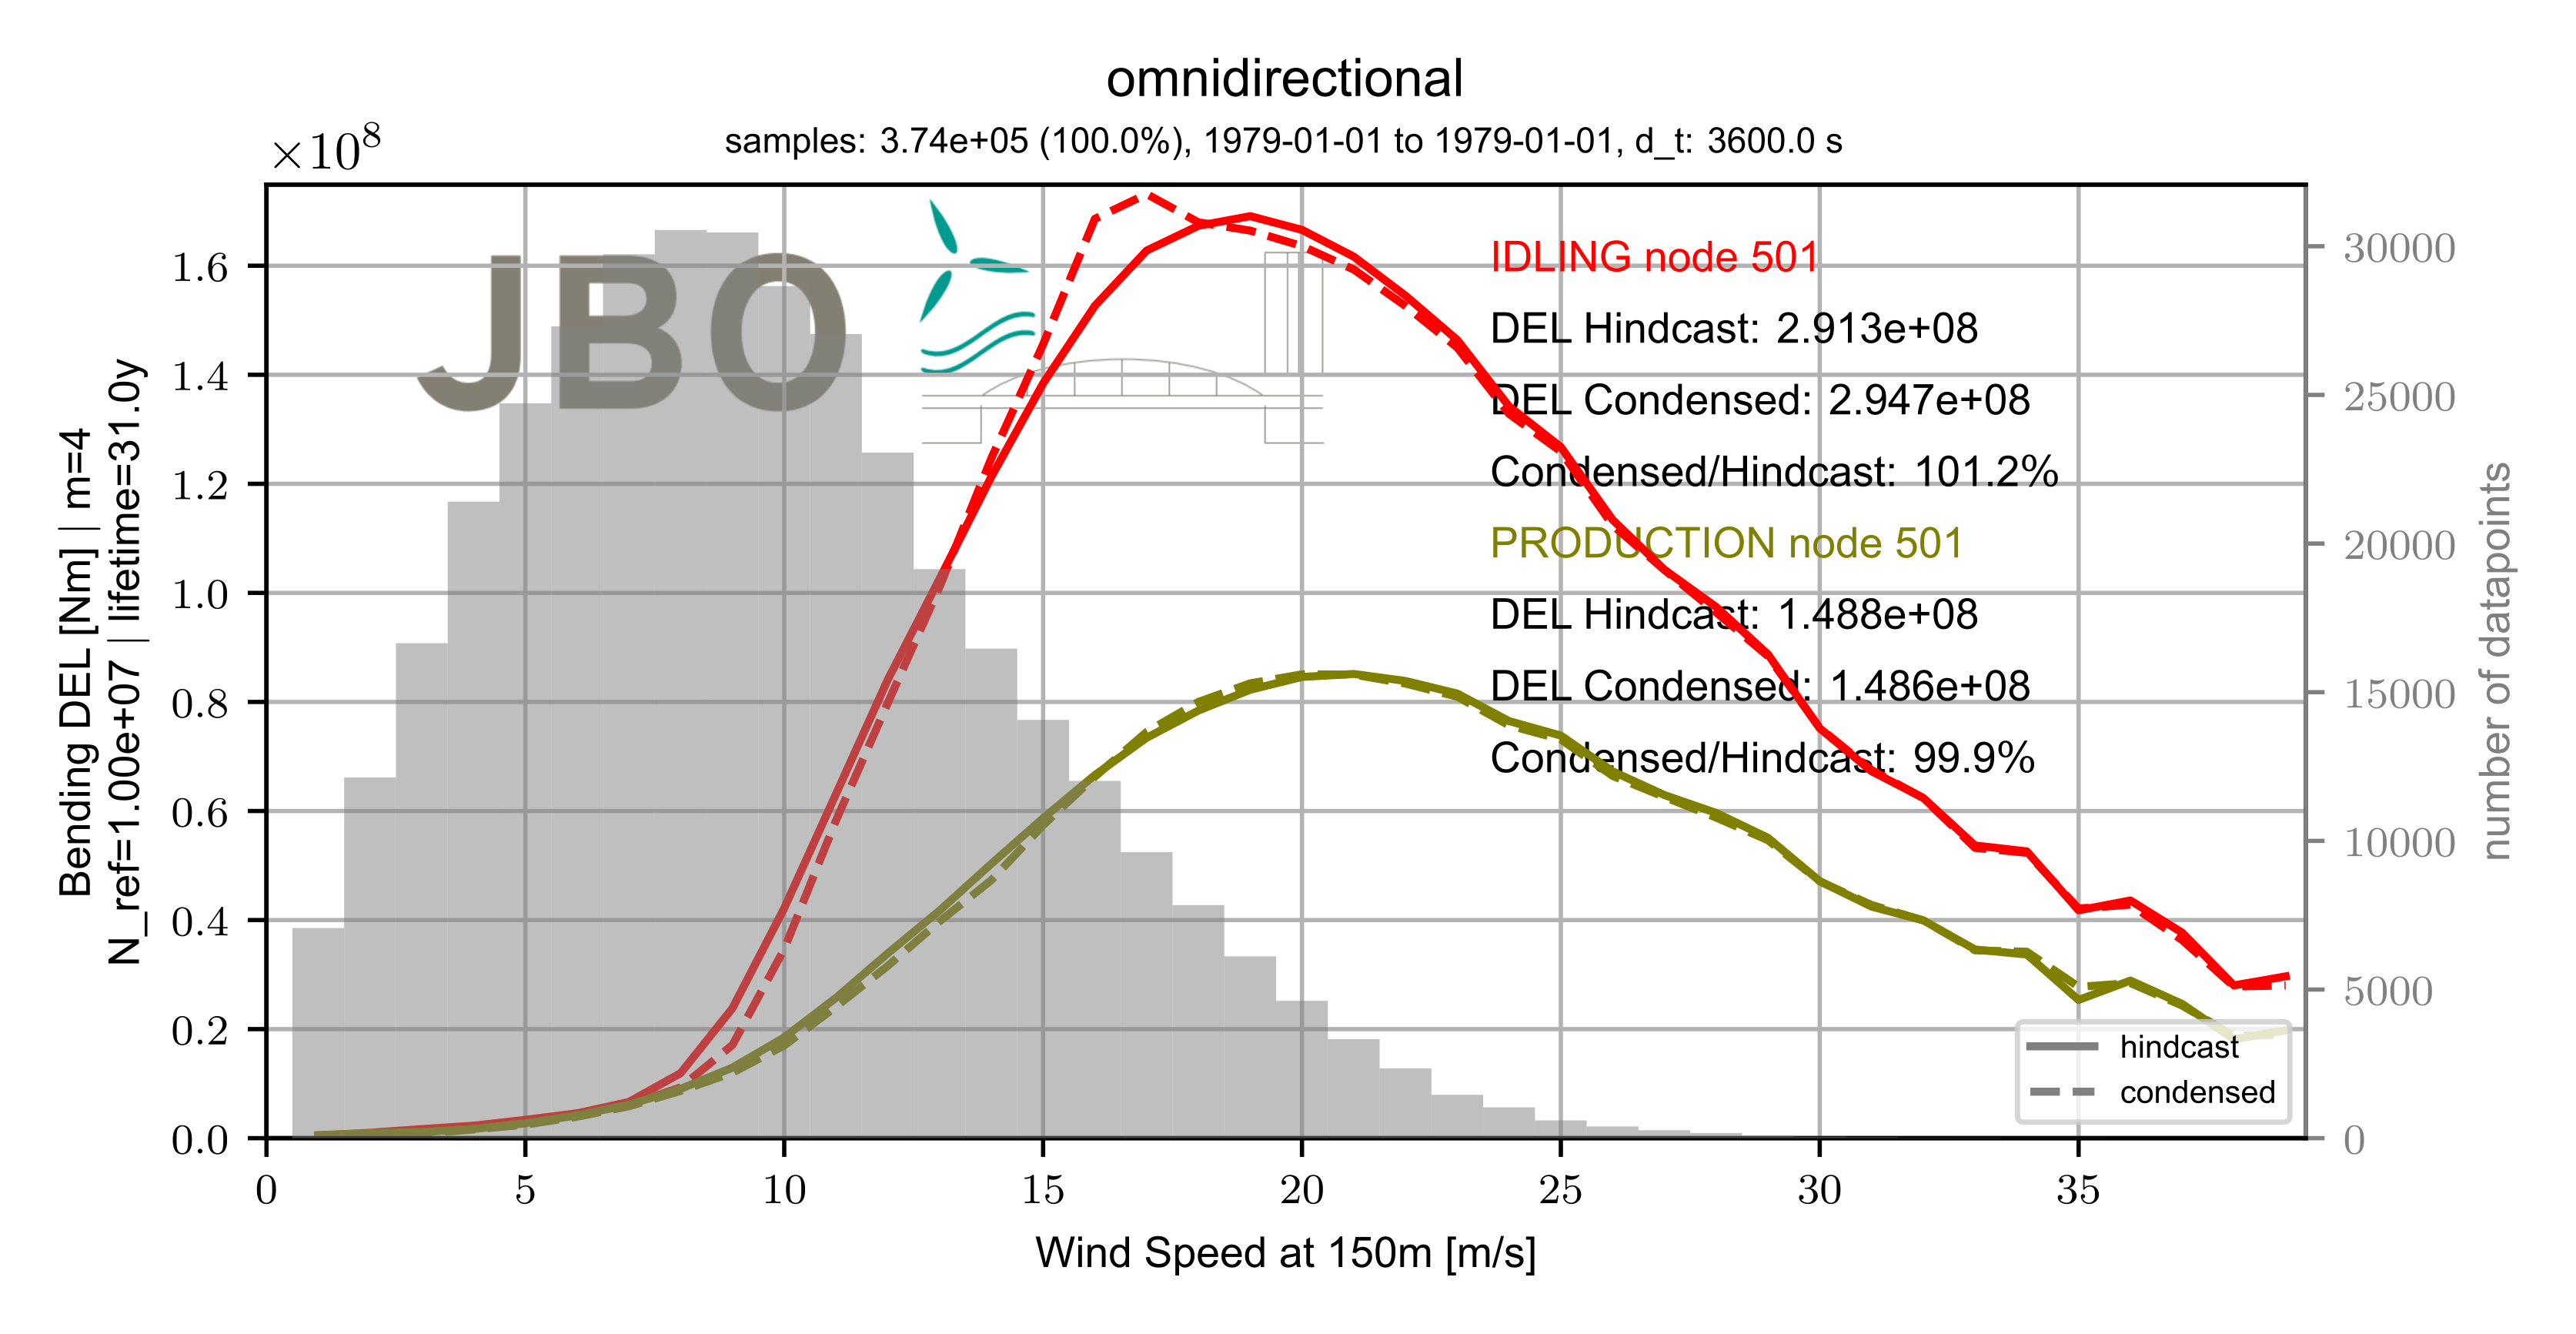
\includegraphics[width=1.0\textwidth]{C:/Users/aaron.lange/Desktop/Projekte/Hindcast_Tool/HindTool/example_output/Valid_line_wind_page_3.png} 
 \caption{ Valid-line-wind-page-3 } 
 \label{fig: Valid_line_wind_page_3 } 
\end{figure}

\begin{figure}[H] 
 \centering 
 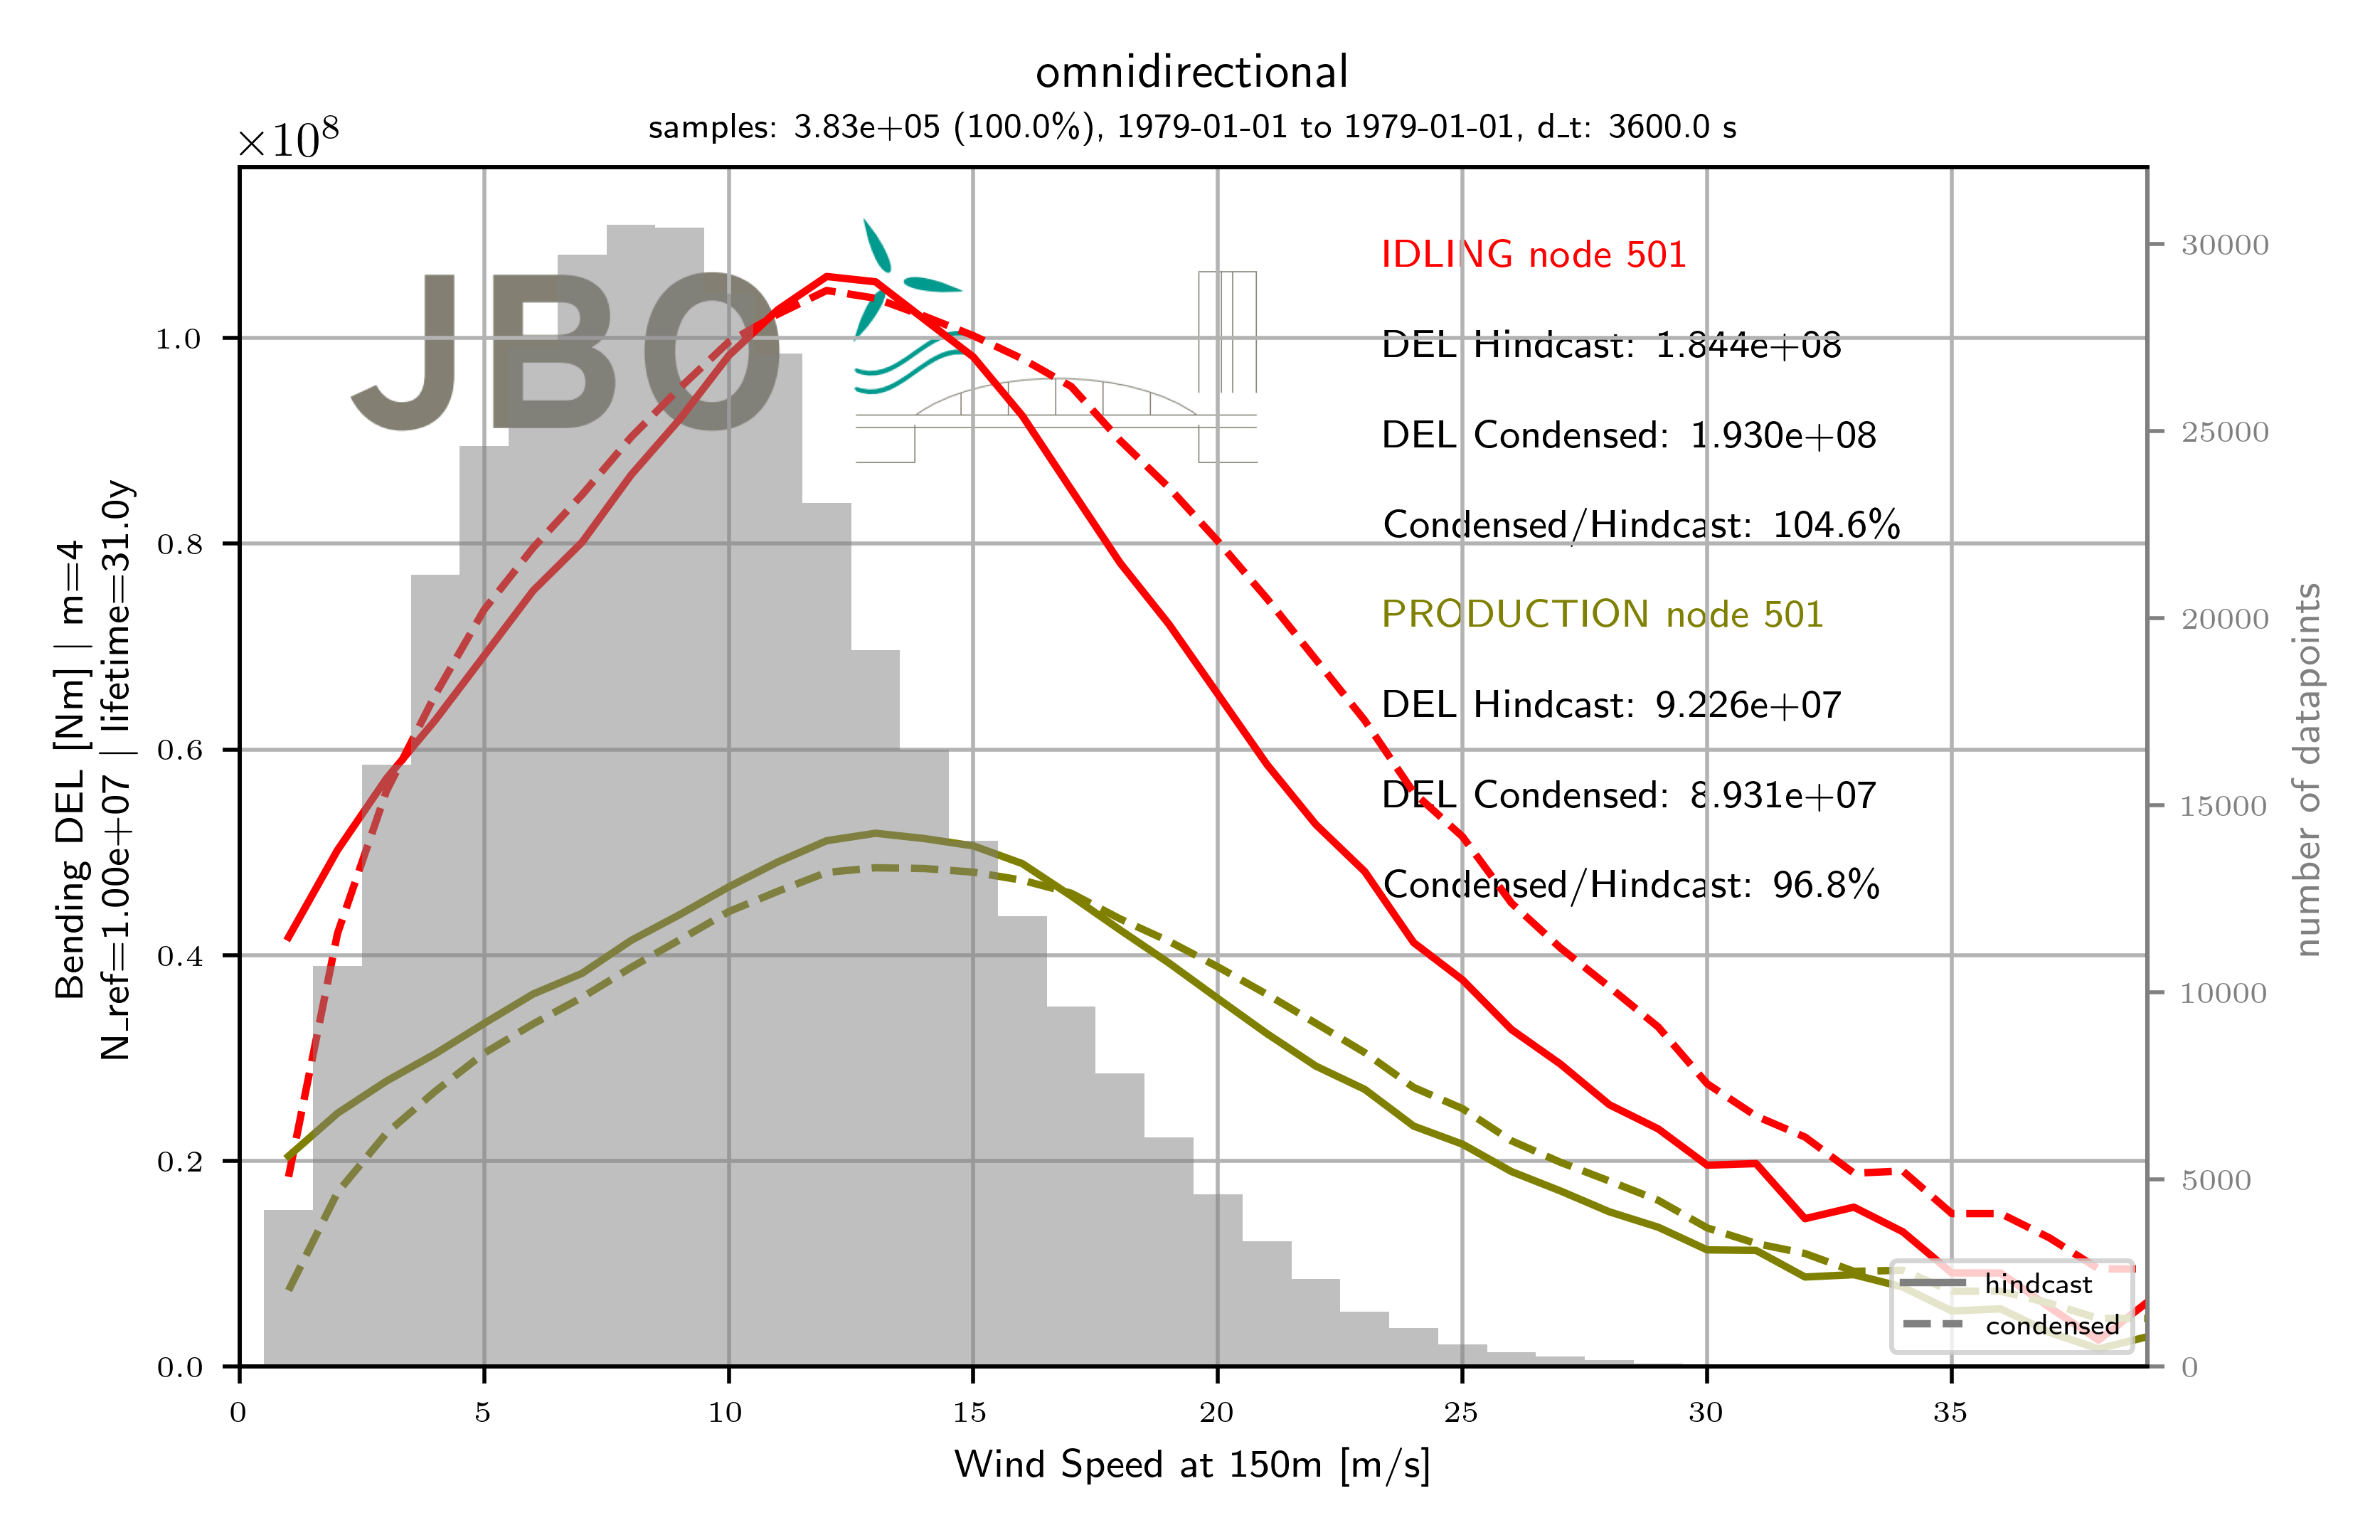
\includegraphics[width=1.0\textwidth]{C:/Users/aaron.lange/Desktop/Projekte/Hindcast_Tool/HindTool/example_output/Valid_line_swell_page_3.png} 
 \caption{ Valid-line-swell-page-3 } 
 \label{fig: Valid_line_swell_page_3 } 
\end{figure}

\begin{figure}[H] 
 \centering 
 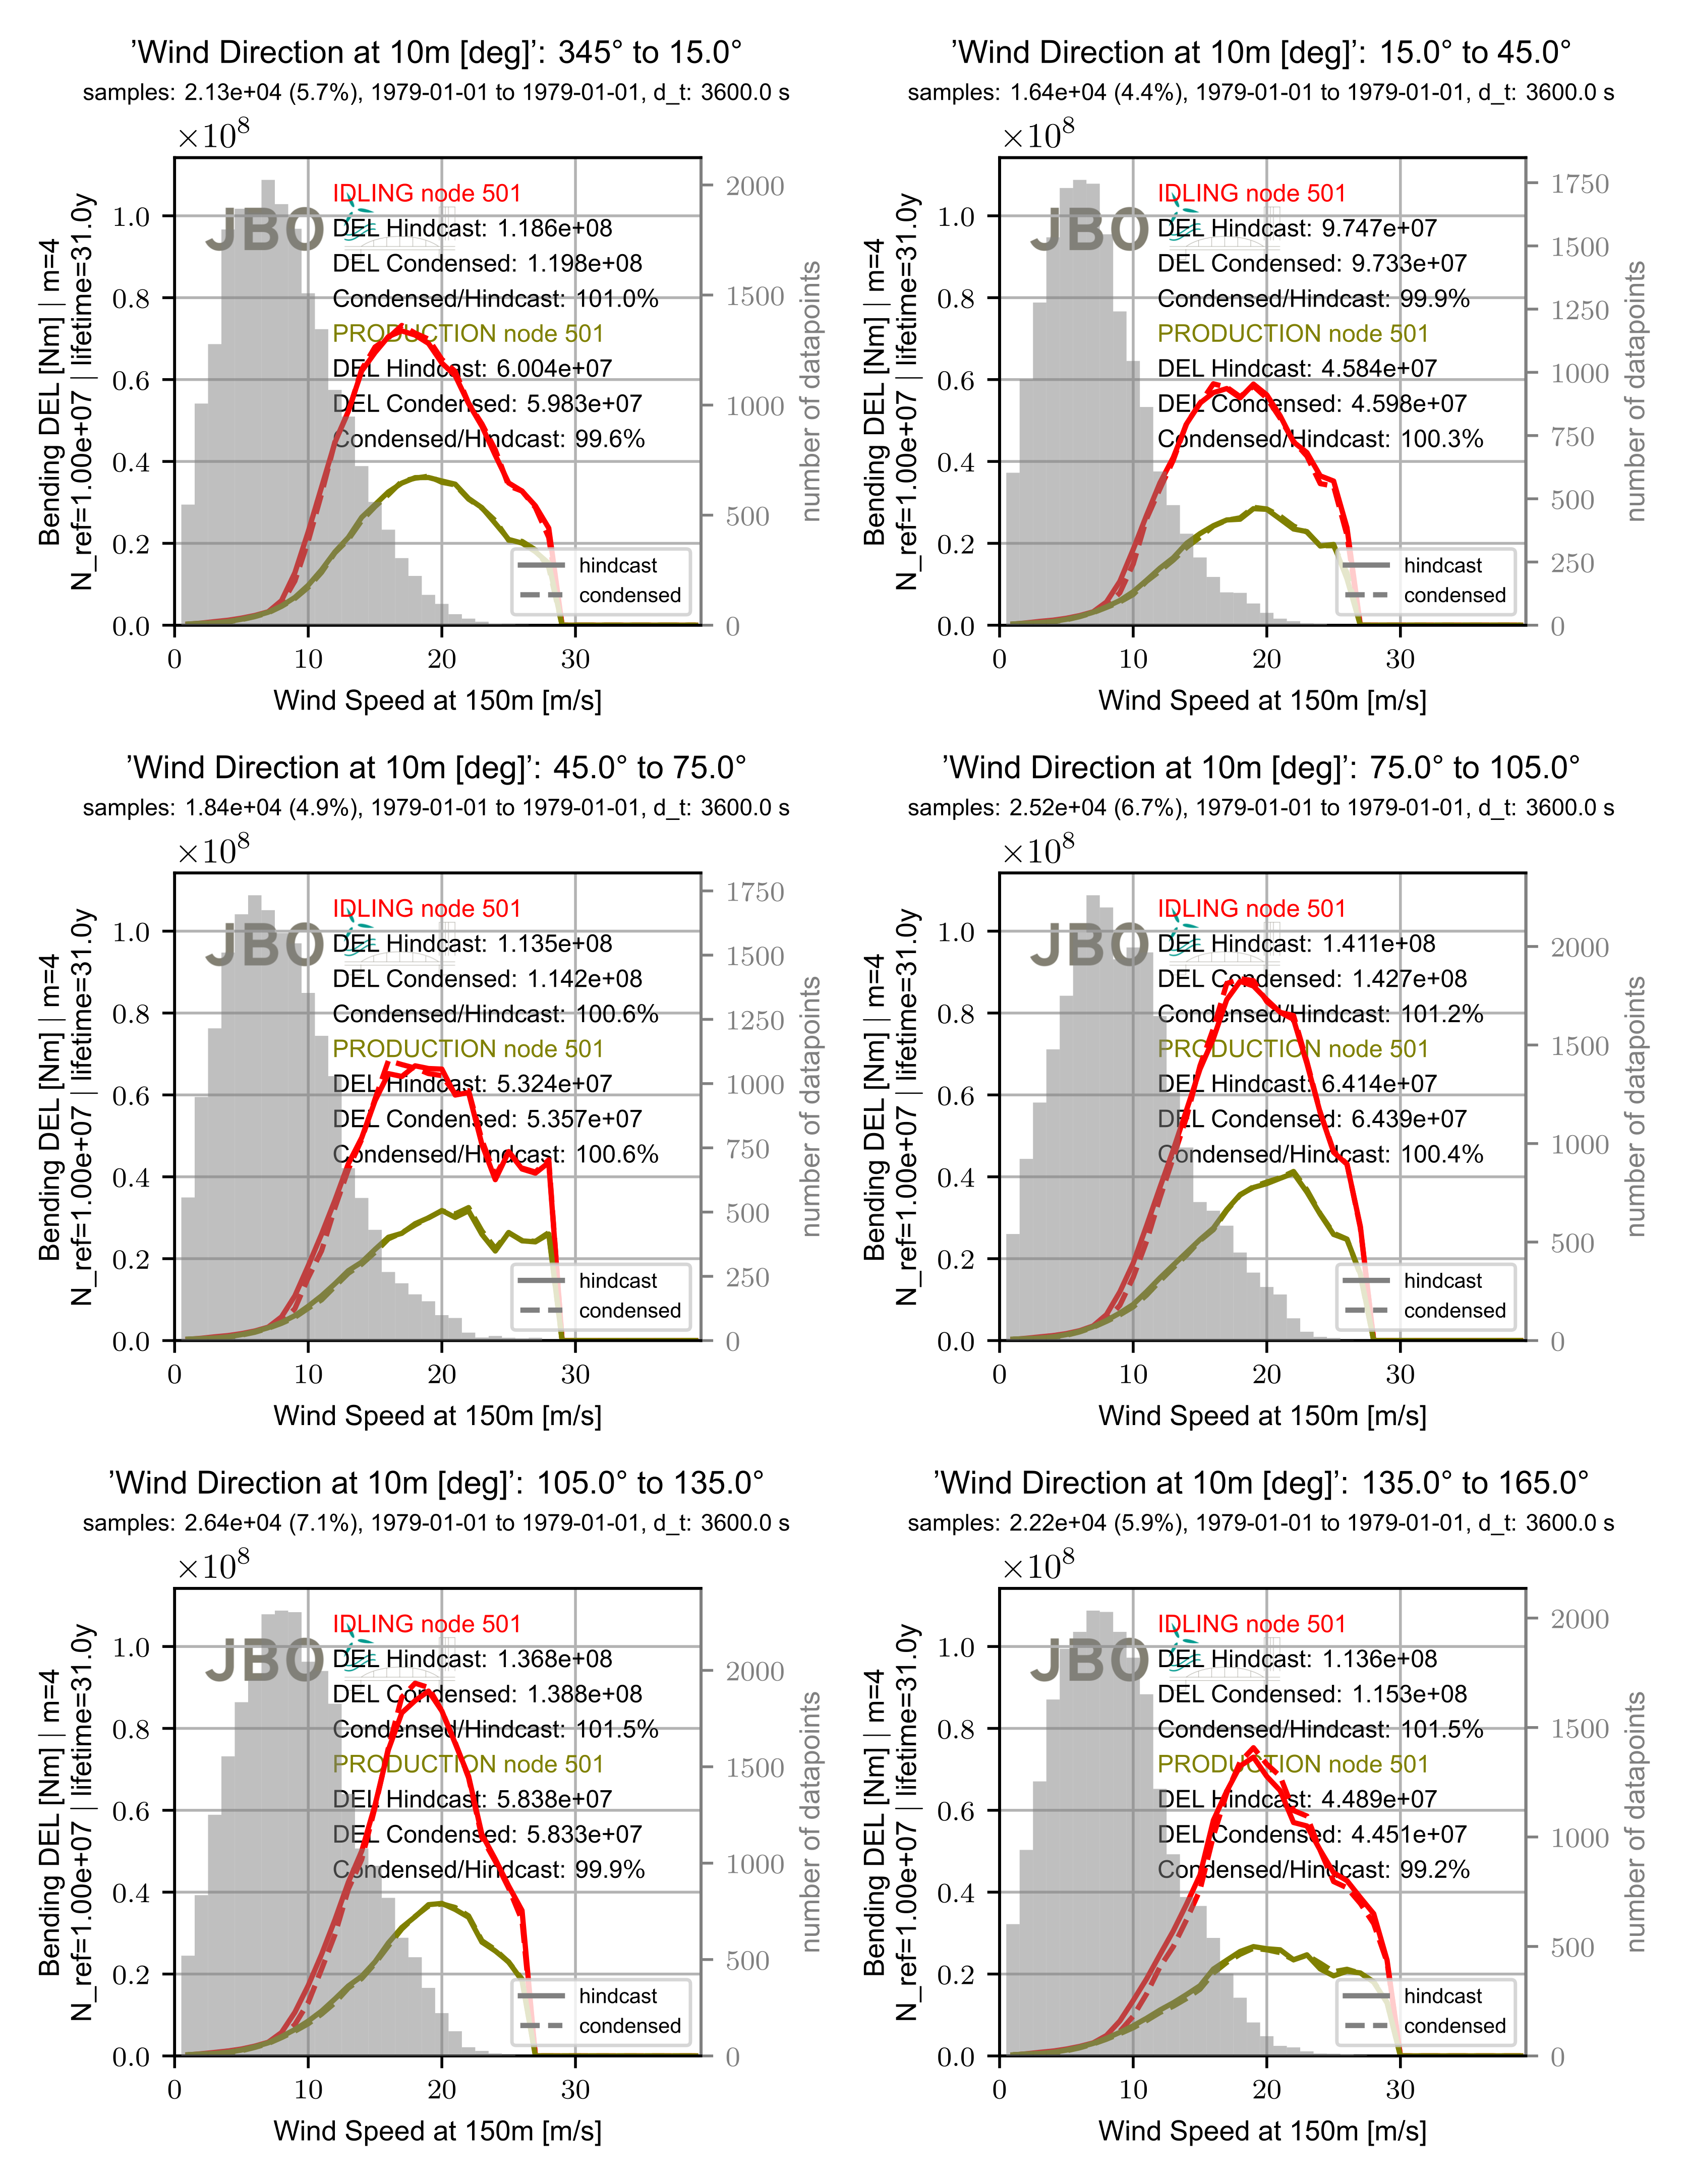
\includegraphics[width=1.0\textwidth]{C:/Users/aaron.lange/Desktop/Projekte/Hindcast_Tool/HindTool/example_output/Valid_line_wind_page_1.png} 
 \caption{ Valid-line-wind-page-1 } 
 \label{fig: Valid_line_wind_page_1 } 
\end{figure}
\begin{figure}[H] 
 \centering 
 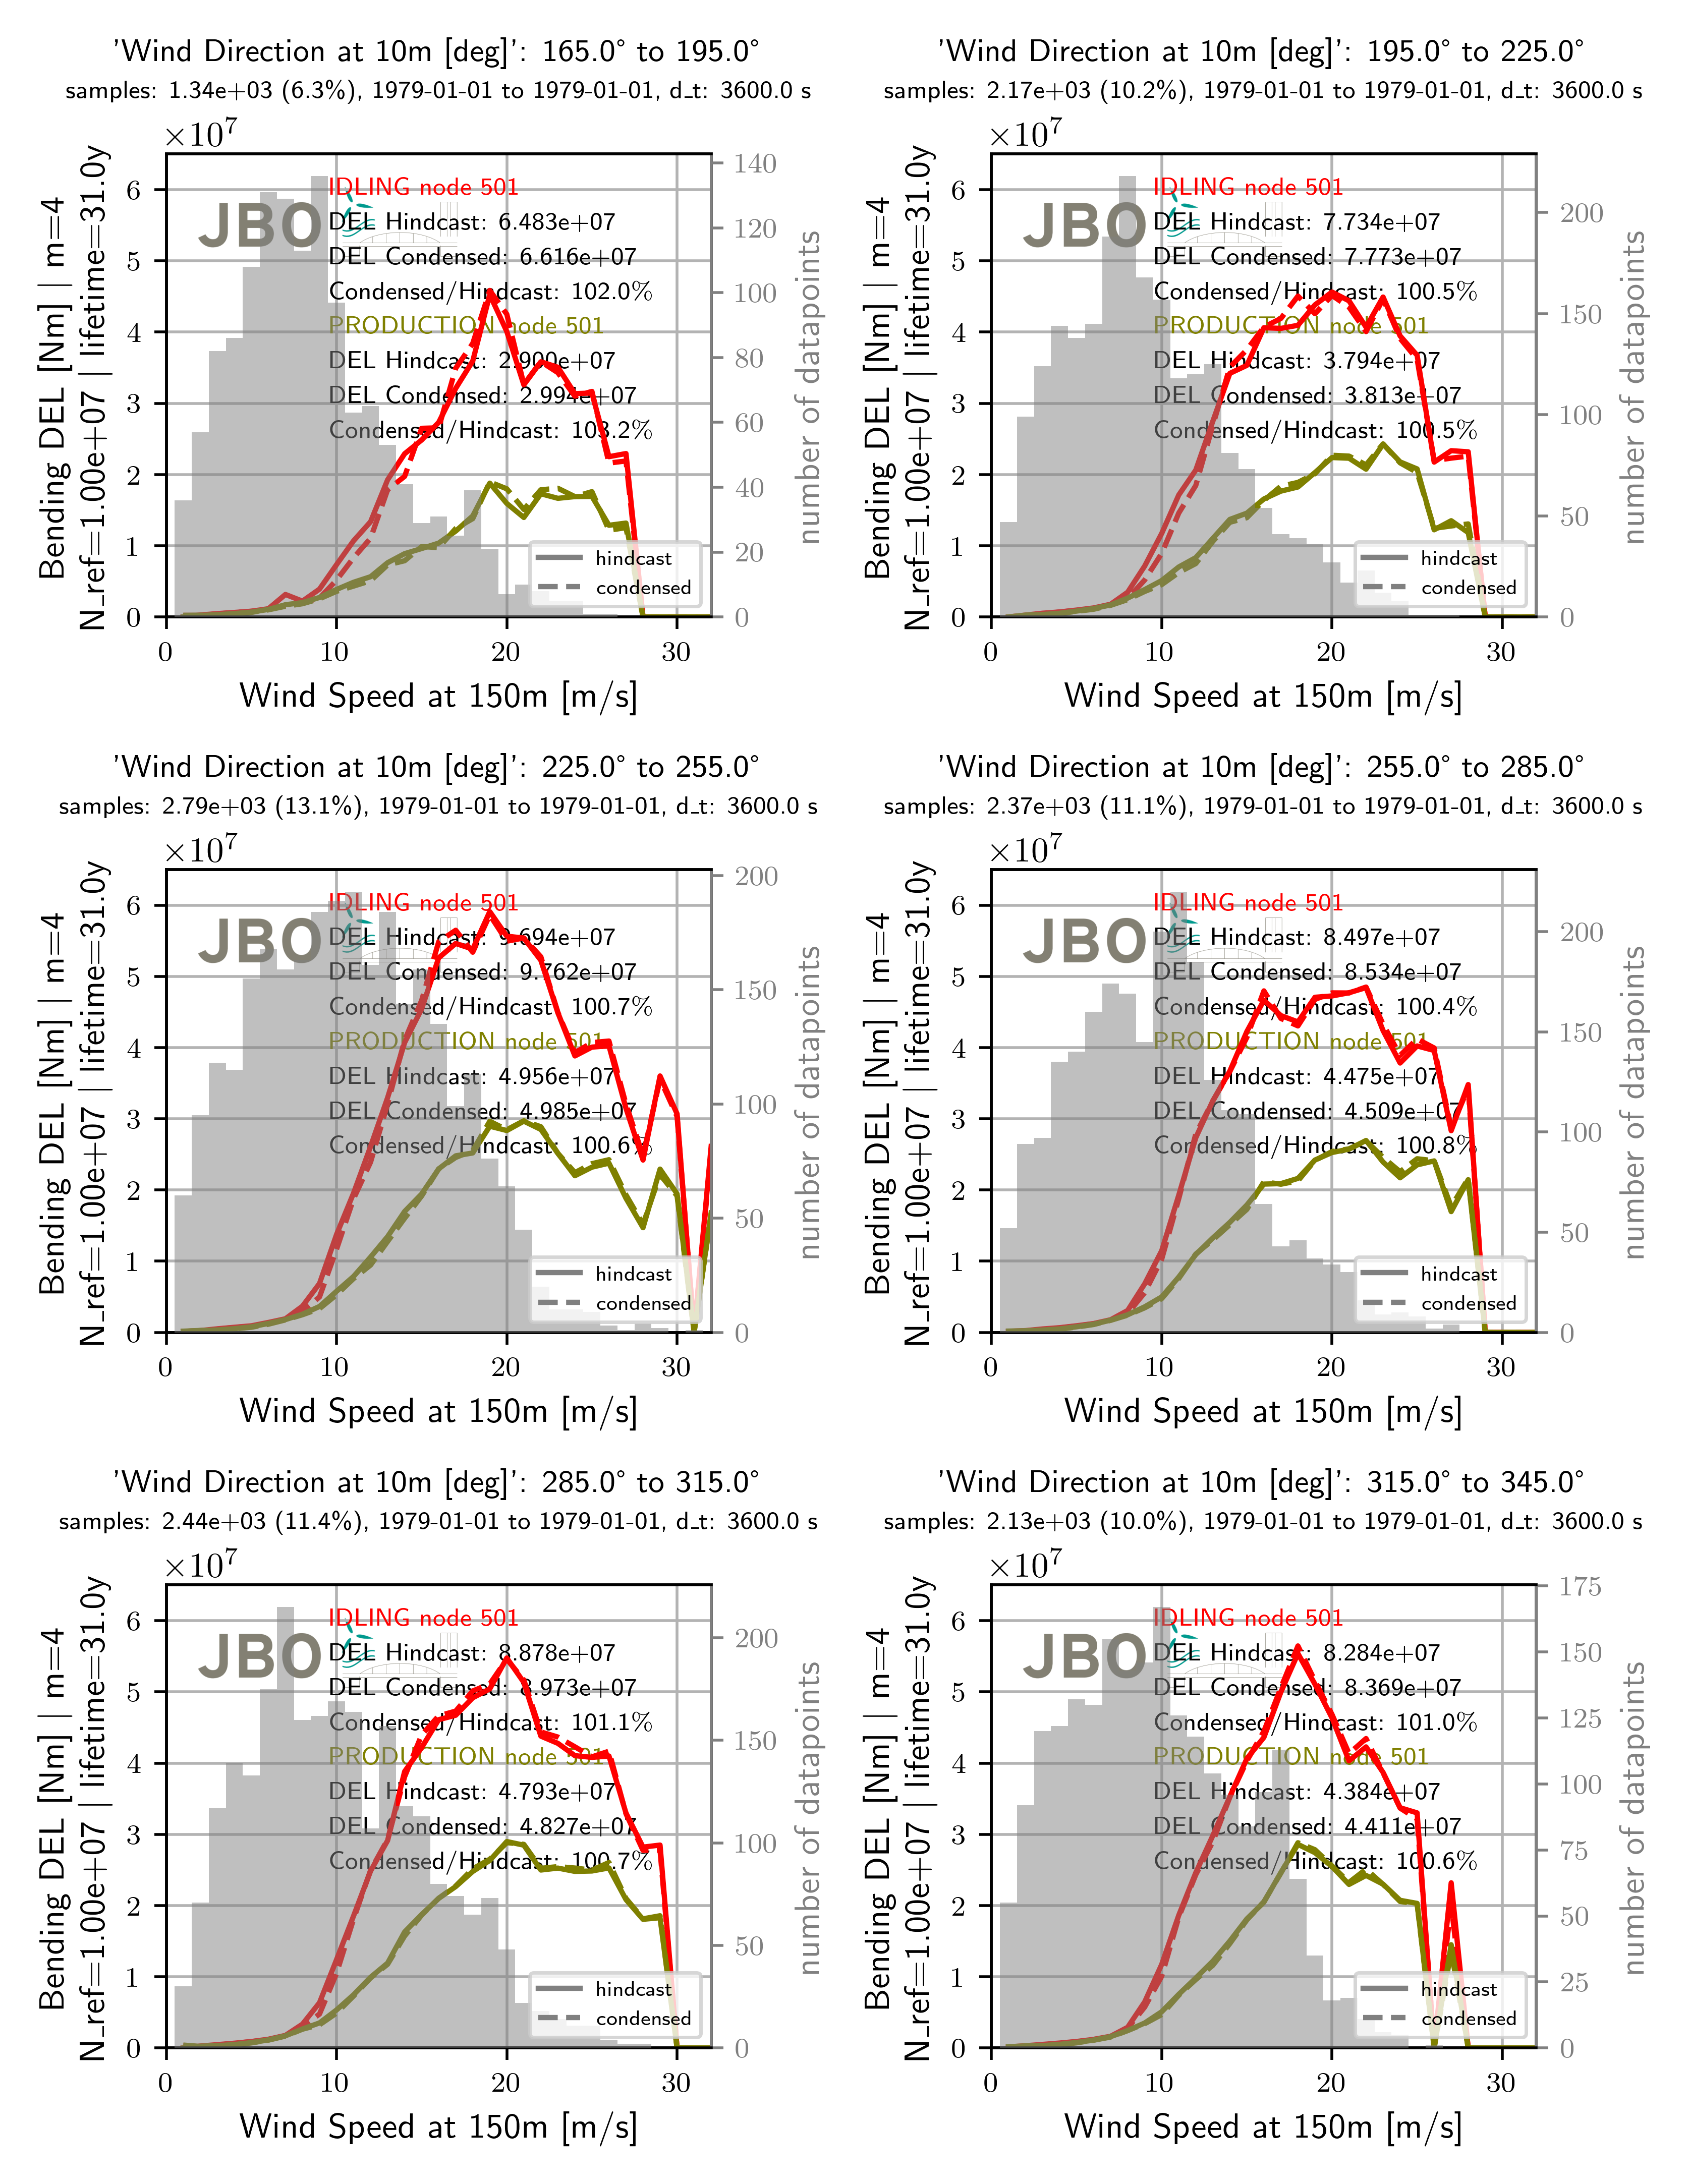
\includegraphics[width=1.0\textwidth]{C:/Users/aaron.lange/Desktop/Projekte/Hindcast_Tool/HindTool/example_output/Valid_line_wind_page_2.png} 
 \caption{ Valid-line-wind-page-2 } 
 \label{fig: Valid_line_wind_page_2 } 
\end{figure}
\begin{figure}[H] 
 \centering 
 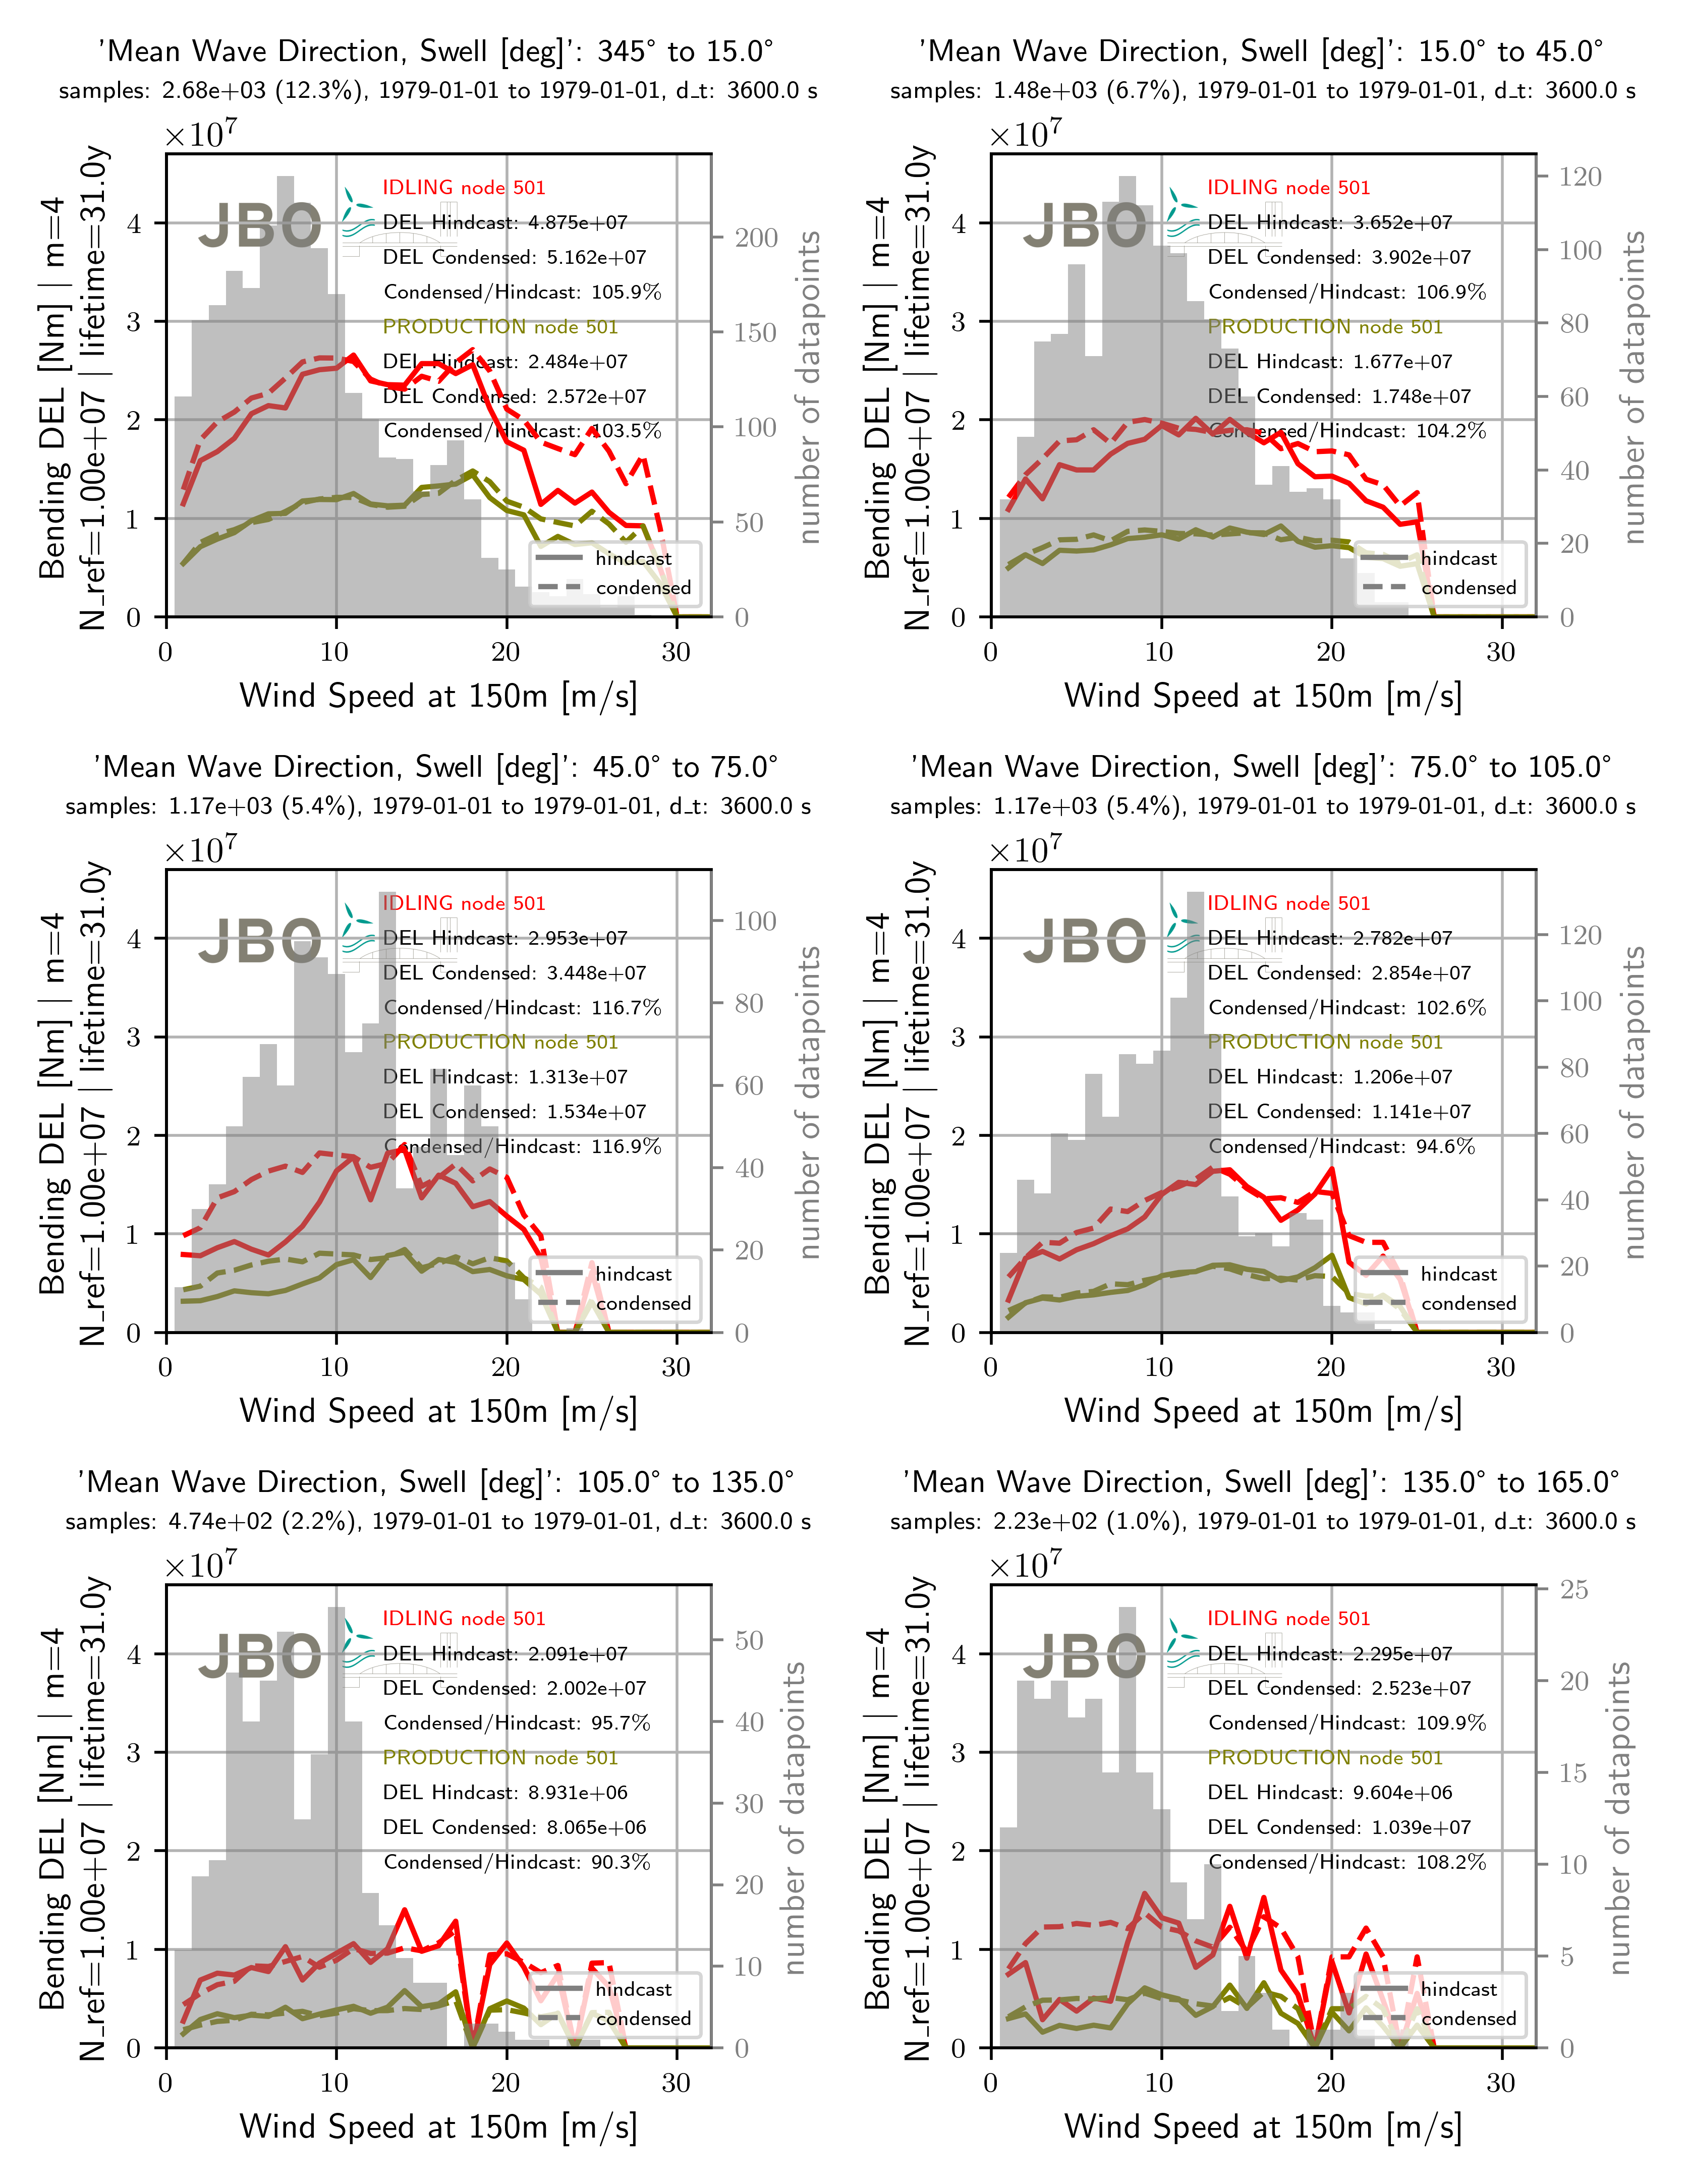
\includegraphics[width=1.0\textwidth]{C:/Users/aaron.lange/Desktop/Projekte/Hindcast_Tool/HindTool/example_output/Valid_line_swell_page_1.png} 
 \caption{ Valid-line-swell-page-1 } 
 \label{fig: Valid_line_swell_page_1 } 
\end{figure}
\begin{figure}[H] 
 \centering 
 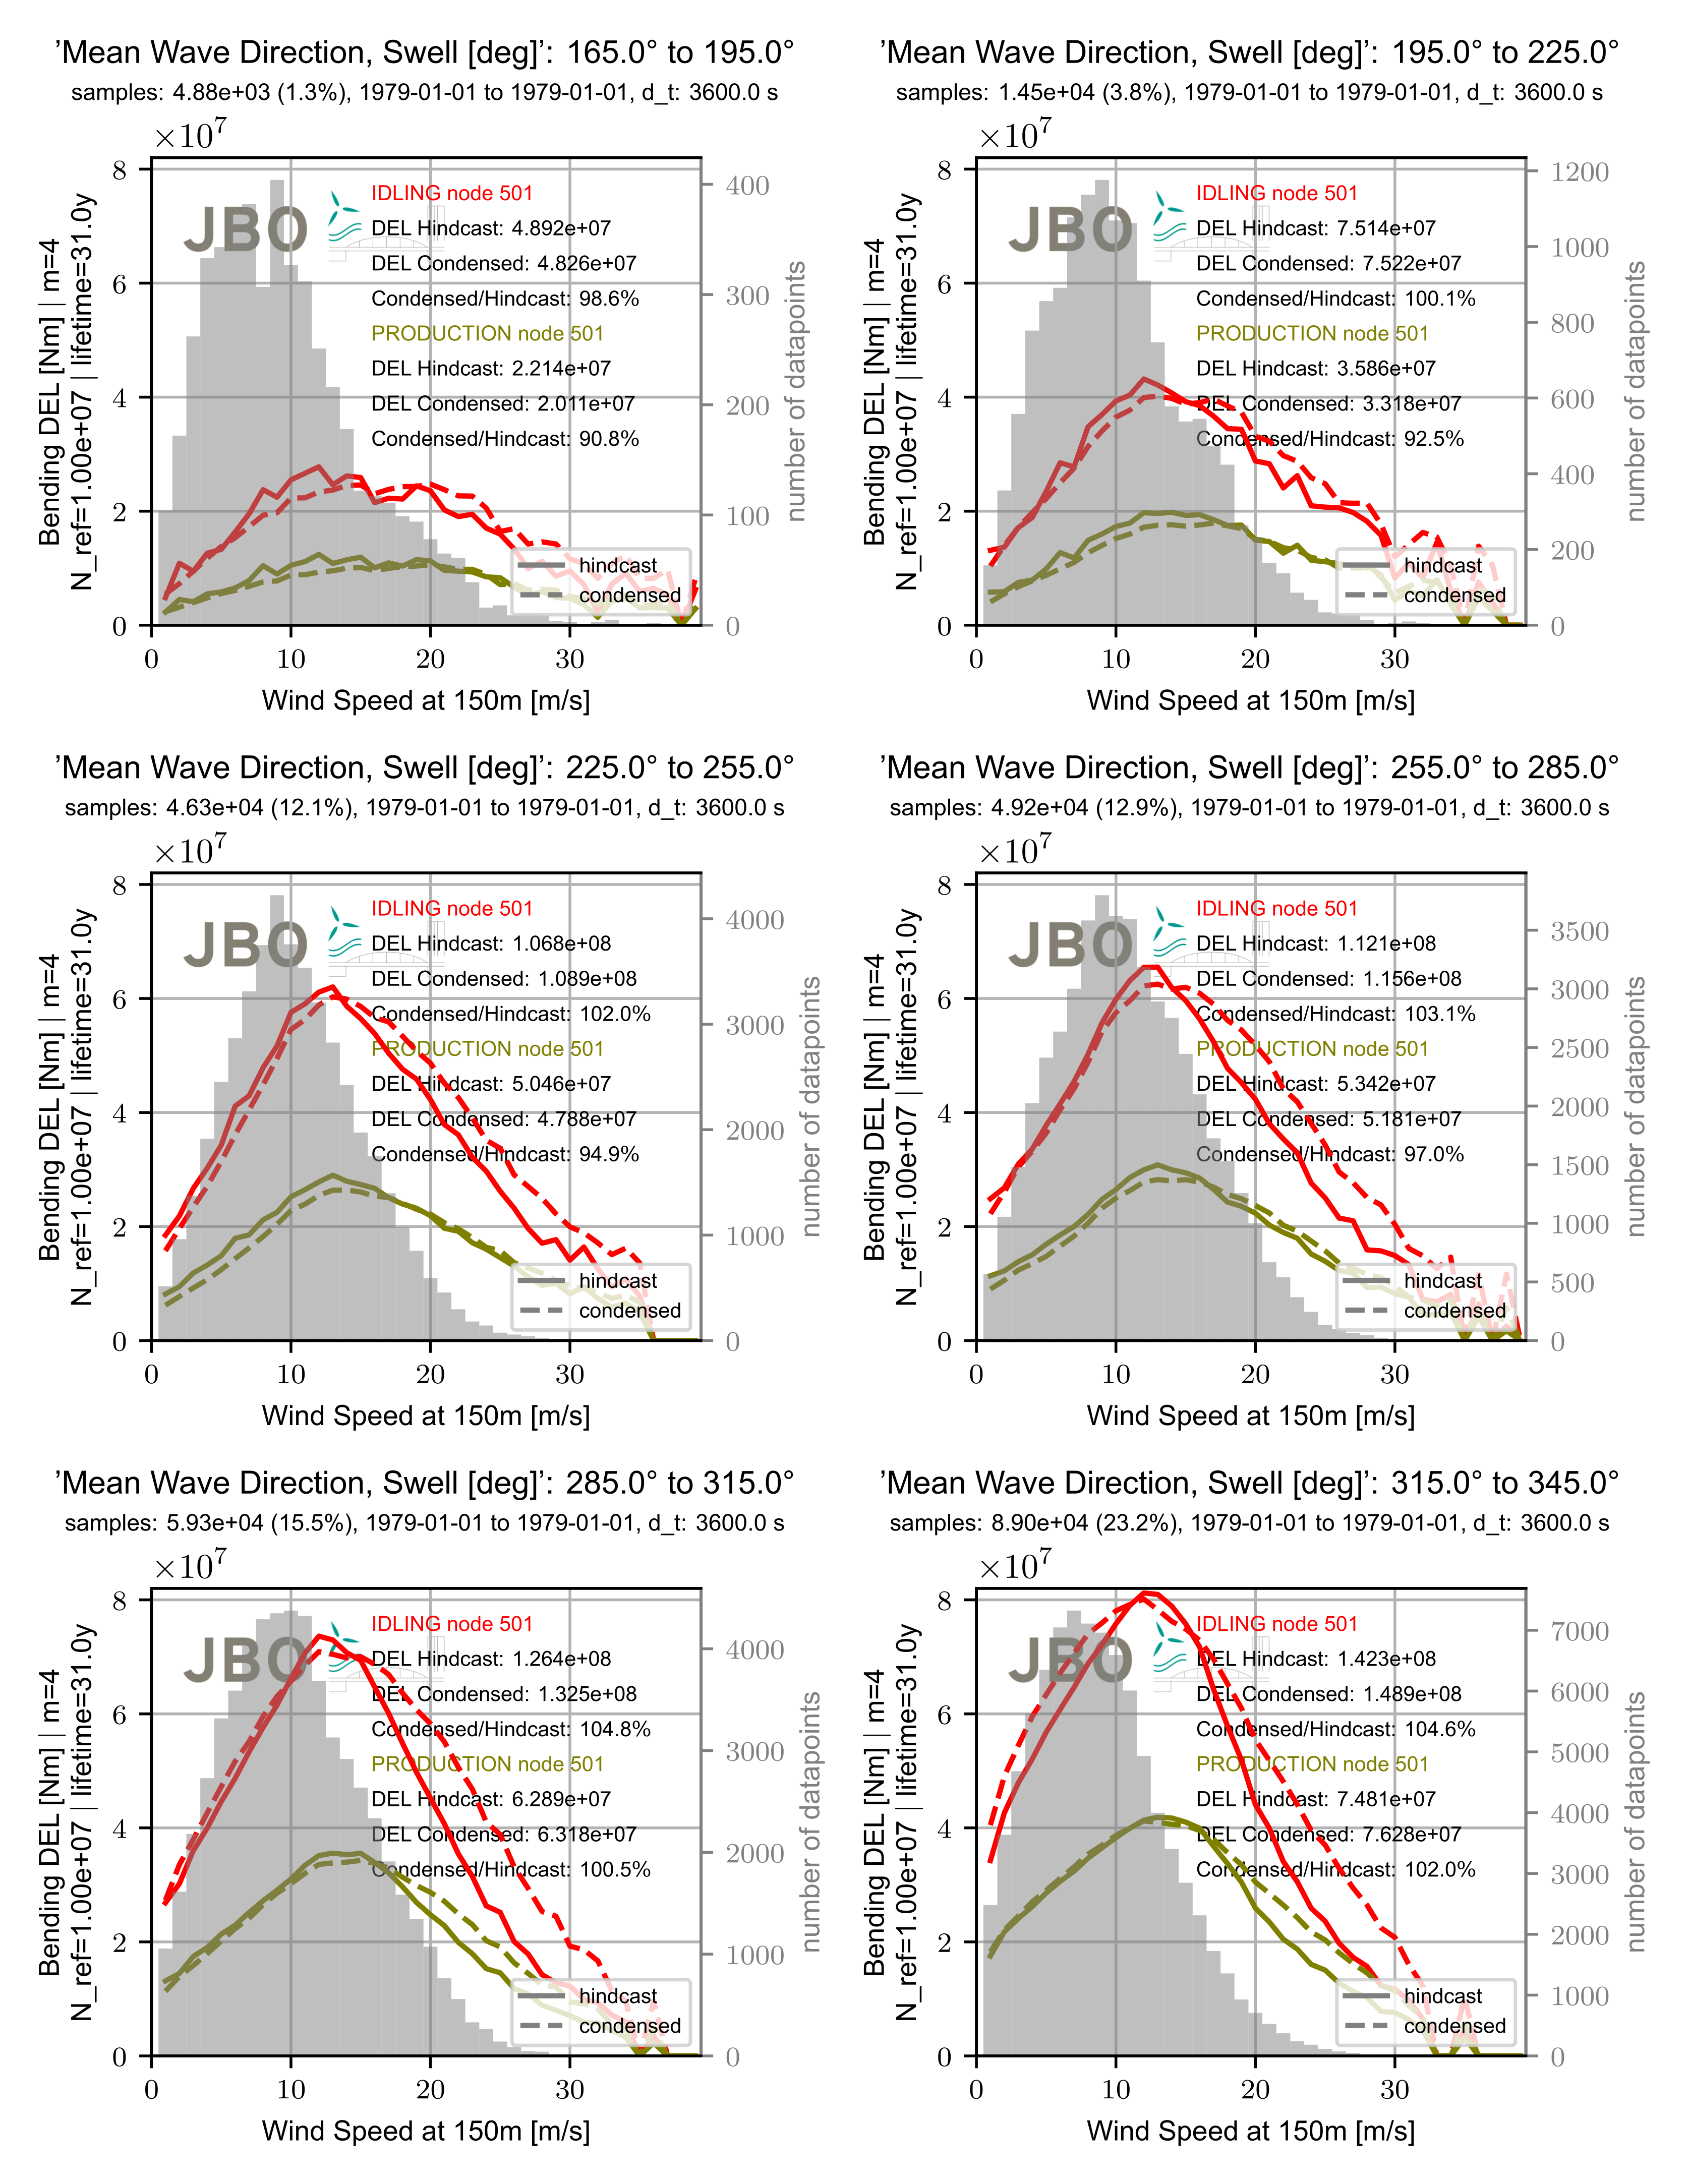
\includegraphics[width=1.0\textwidth]{C:/Users/aaron.lange/Desktop/Projekte/Hindcast_Tool/HindTool/example_output/Valid_line_swell_page_2.png} 
 \caption{ Valid-line-swell-page-2 } 
 \label{fig: Valid_line_swell_page_2 } 
\end{figure}
\begin{figure}[H] 
 \centering 
 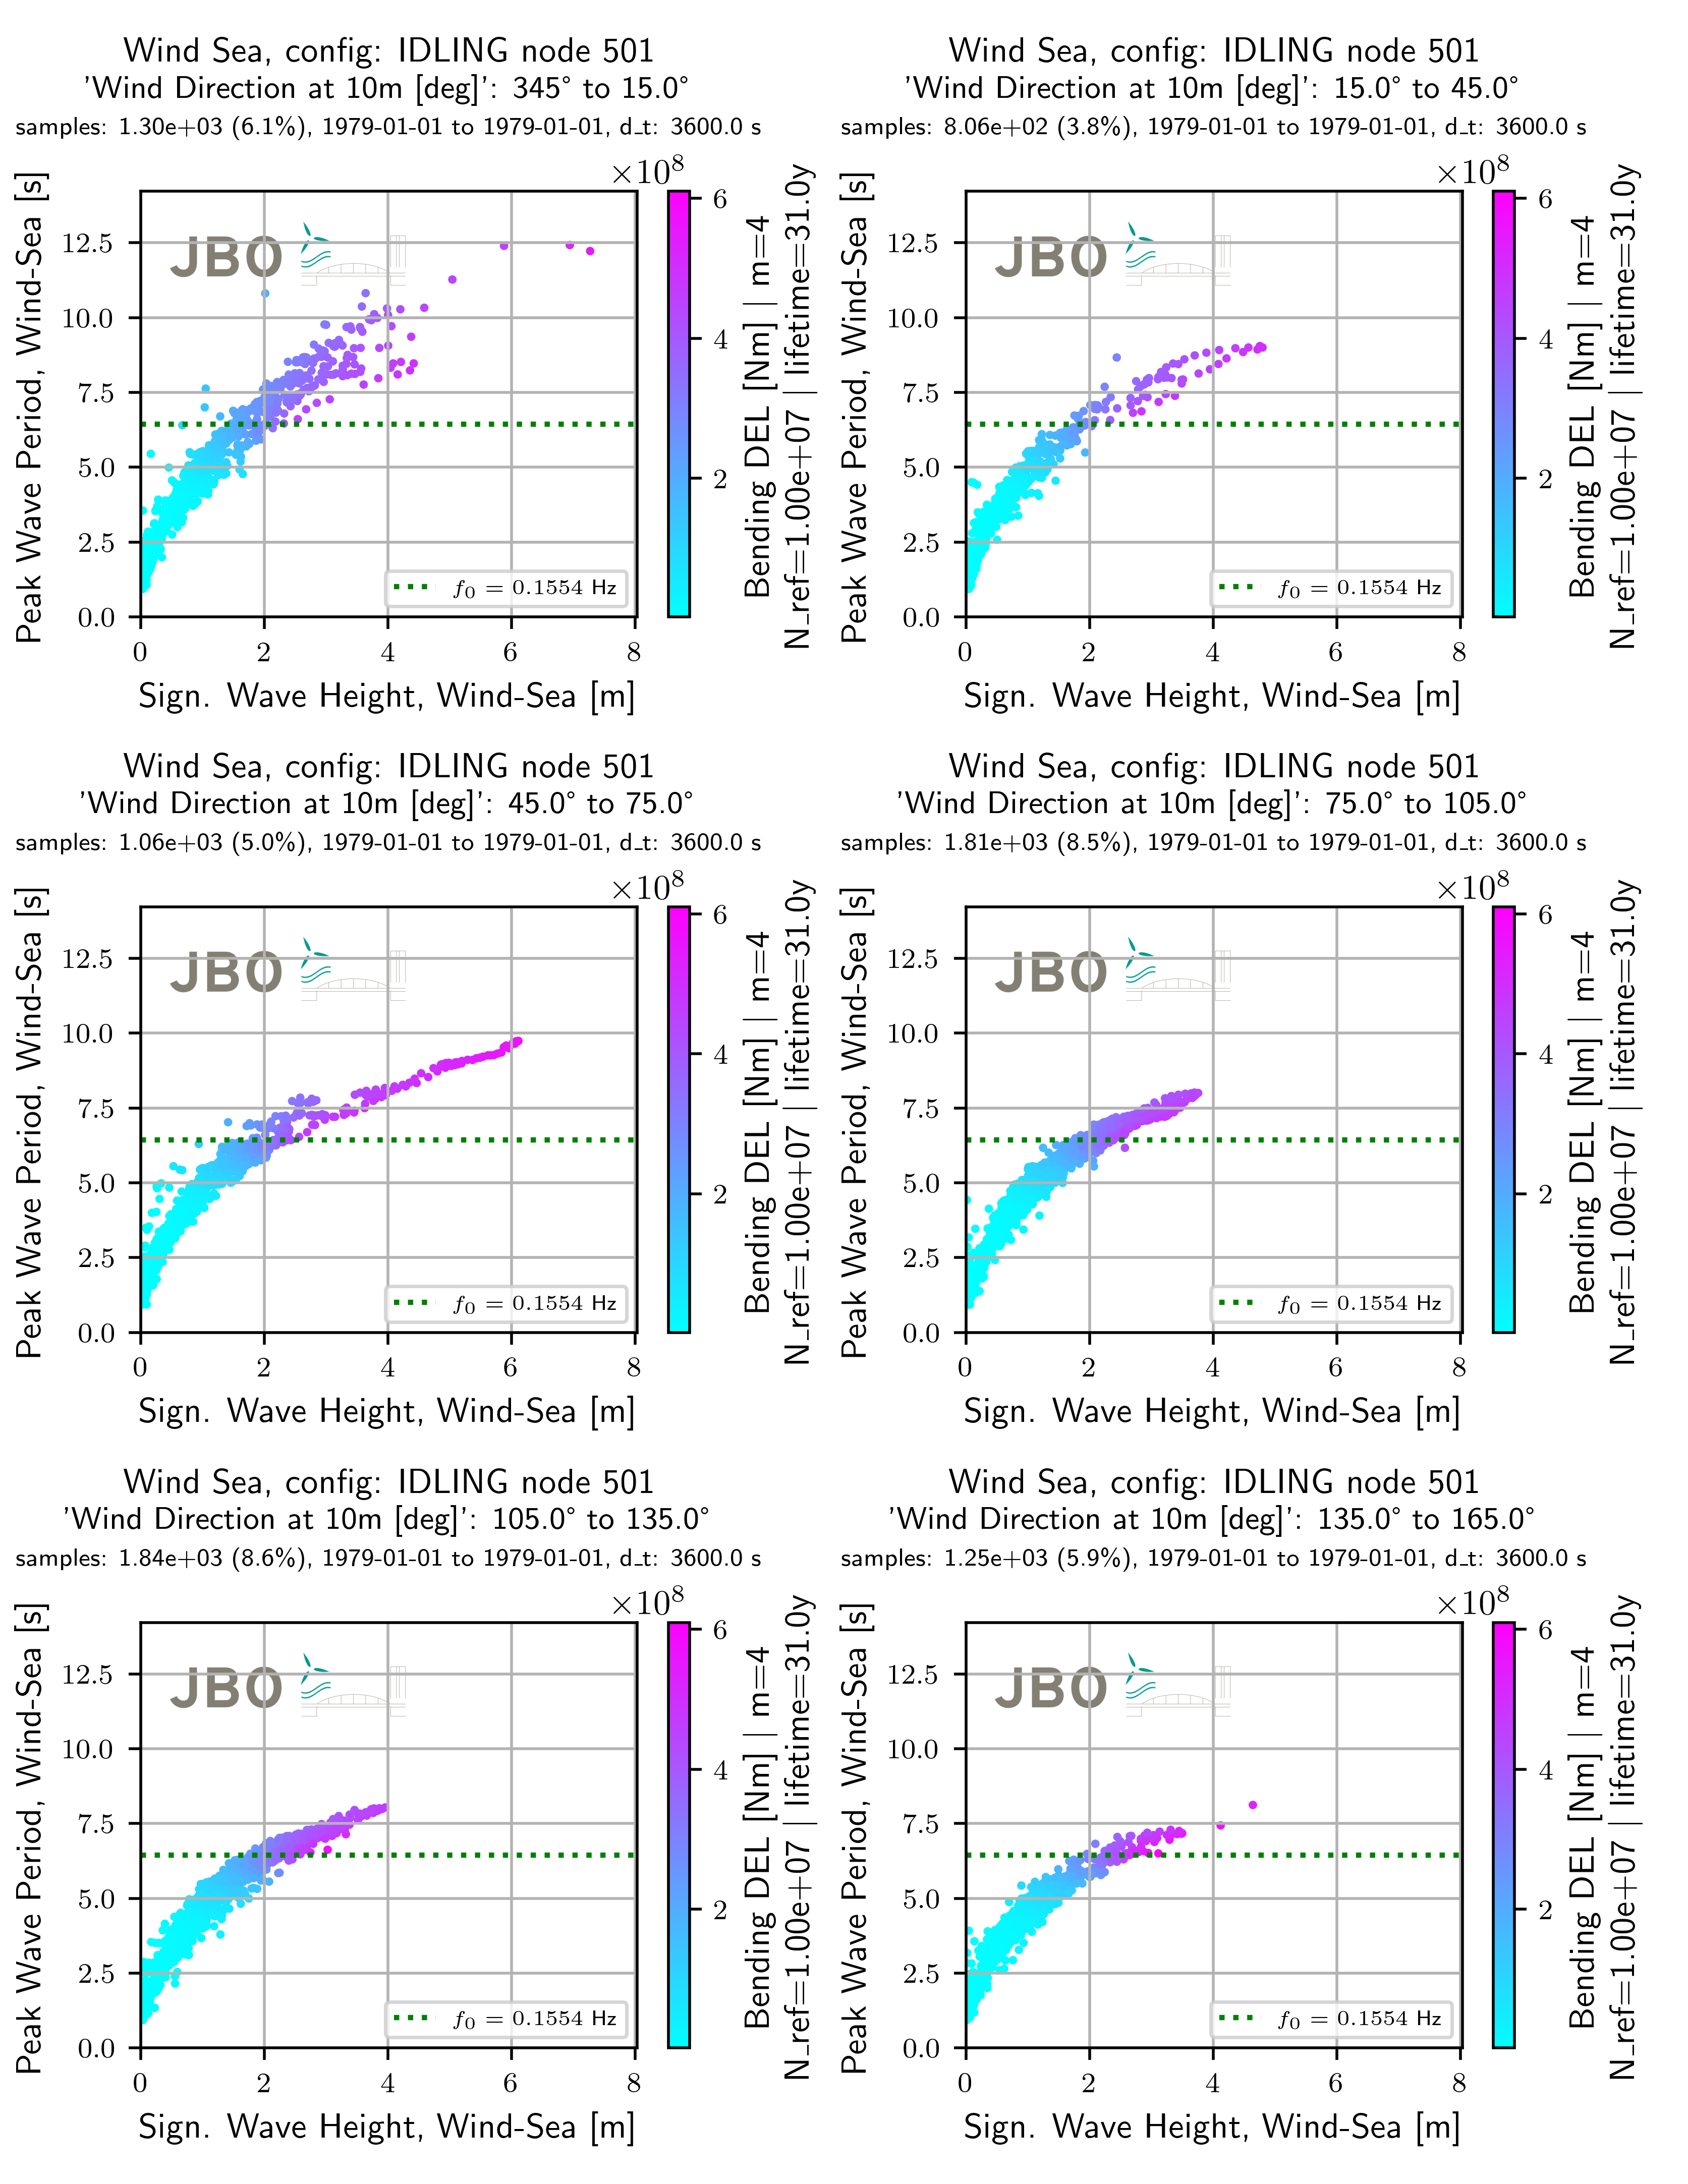
\includegraphics[width=1.0\textwidth]{C:/Users/aaron.lange/Desktop/Projekte/Hindcast_Tool/HindTool/example_output/Valid_scatter_wind_page_1.png} 
 \caption{ Valid-scatter-wind-page-1 } 
 \label{fig: Valid_scatter_wind_page_1 } 
\end{figure}
\begin{figure}[H] 
 \centering 
 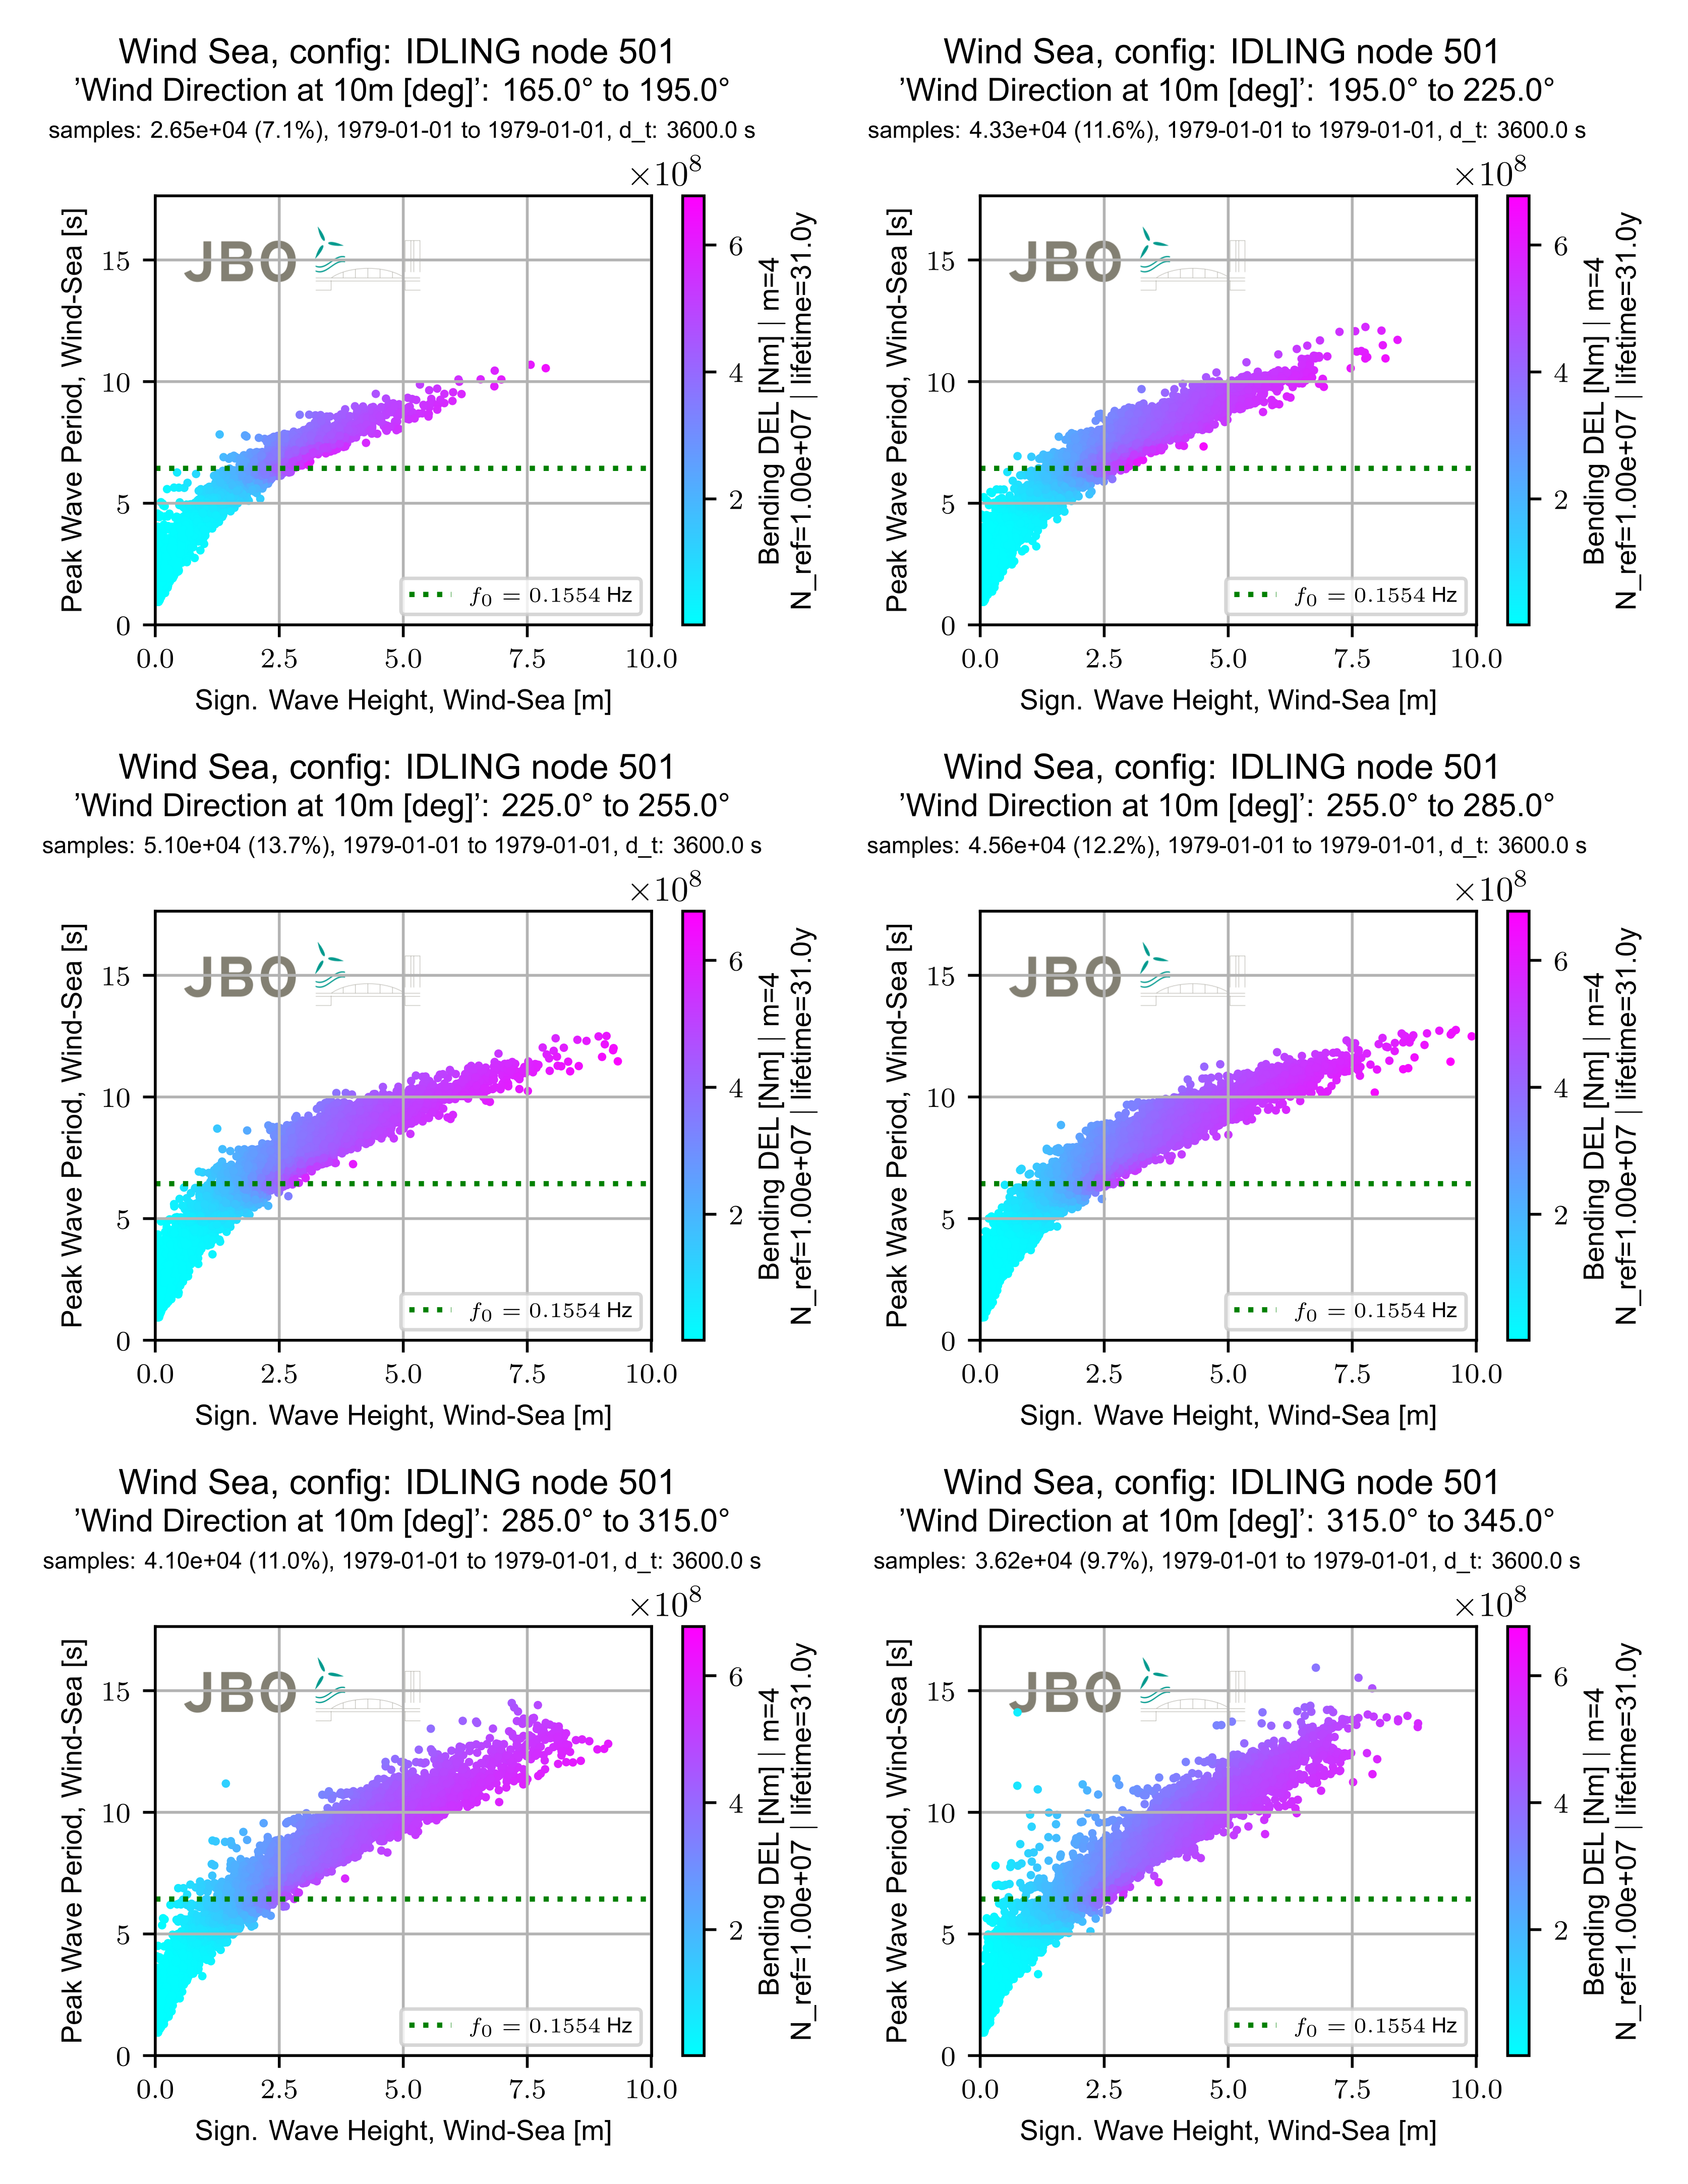
\includegraphics[width=1.0\textwidth]{C:/Users/aaron.lange/Desktop/Projekte/Hindcast_Tool/HindTool/example_output/Valid_scatter_wind_page_2.png} 
 \caption{ Valid-scatter-wind-page-2 } 
 \label{fig: Valid_scatter_wind_page_2 } 
\end{figure}
\begin{figure}[H] 
 \centering 
 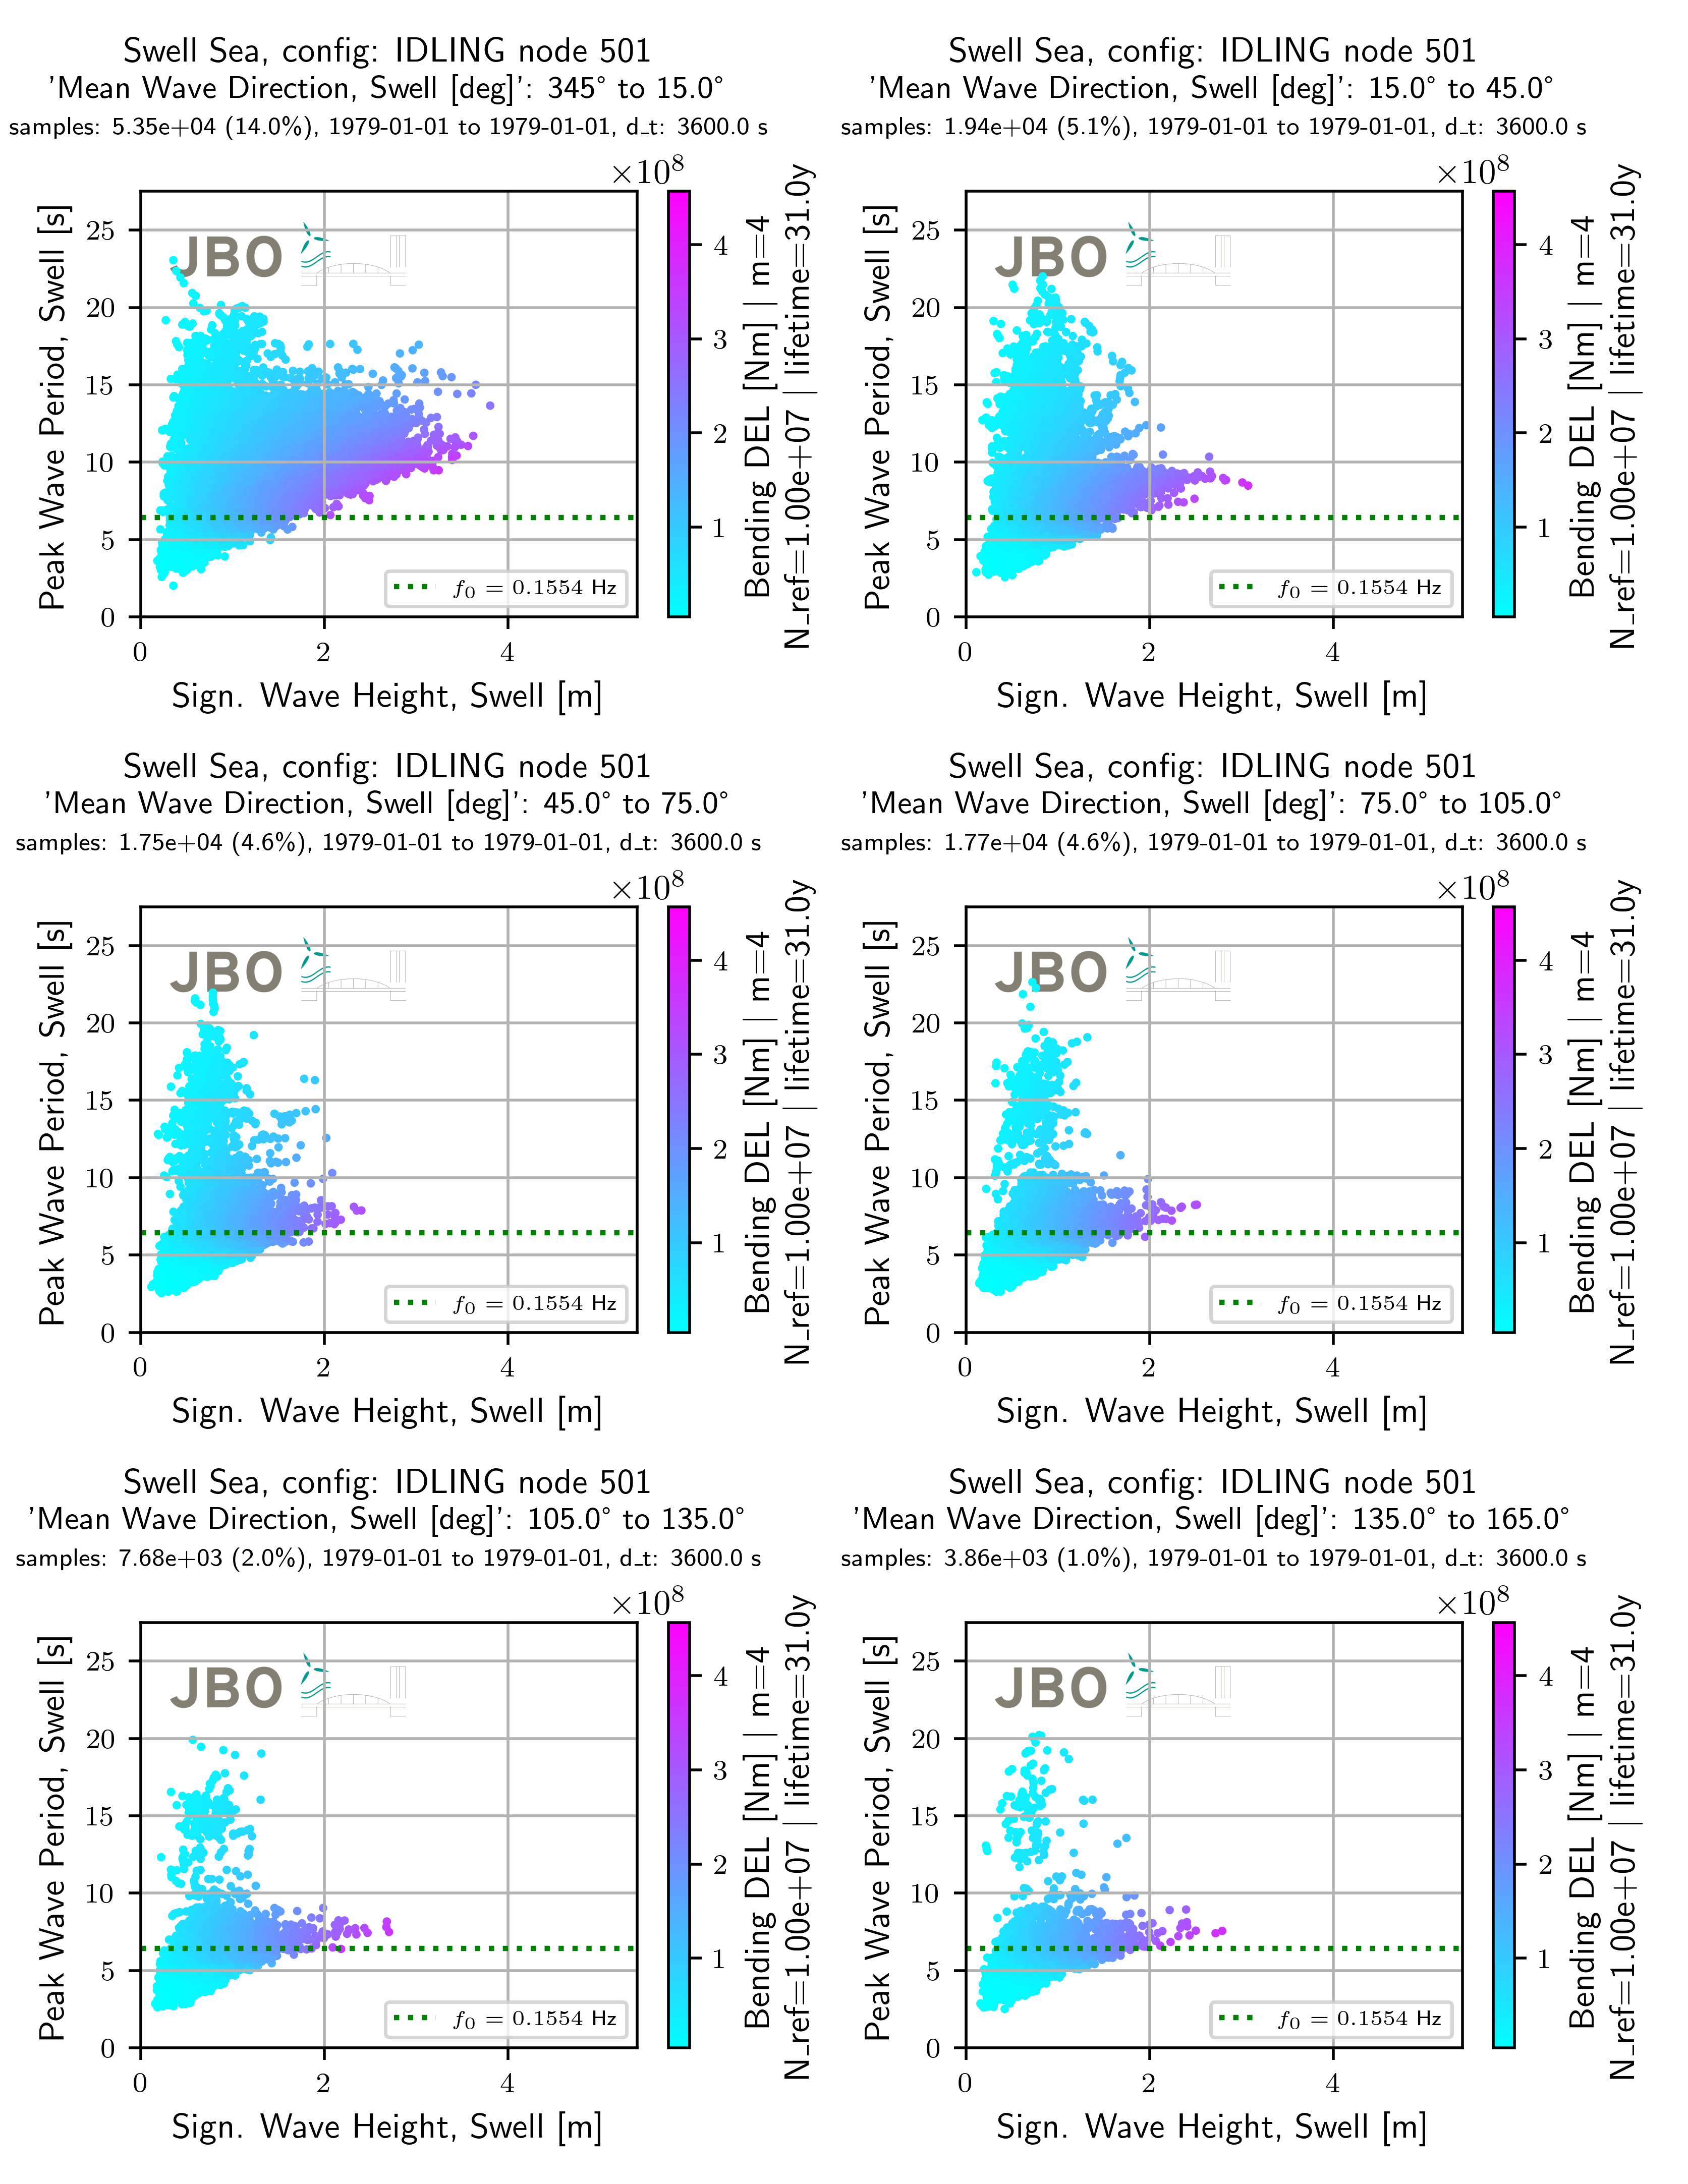
\includegraphics[width=1.0\textwidth]{C:/Users/aaron.lange/Desktop/Projekte/Hindcast_Tool/HindTool/example_output/Valid_scatter_swell_page_1.png} 
 \caption{ Valid-scatter-swell-page-1 } 
 \label{fig: Valid_scatter_swell_page_1 } 
\end{figure}
\begin{figure}[H] 
 \centering 
 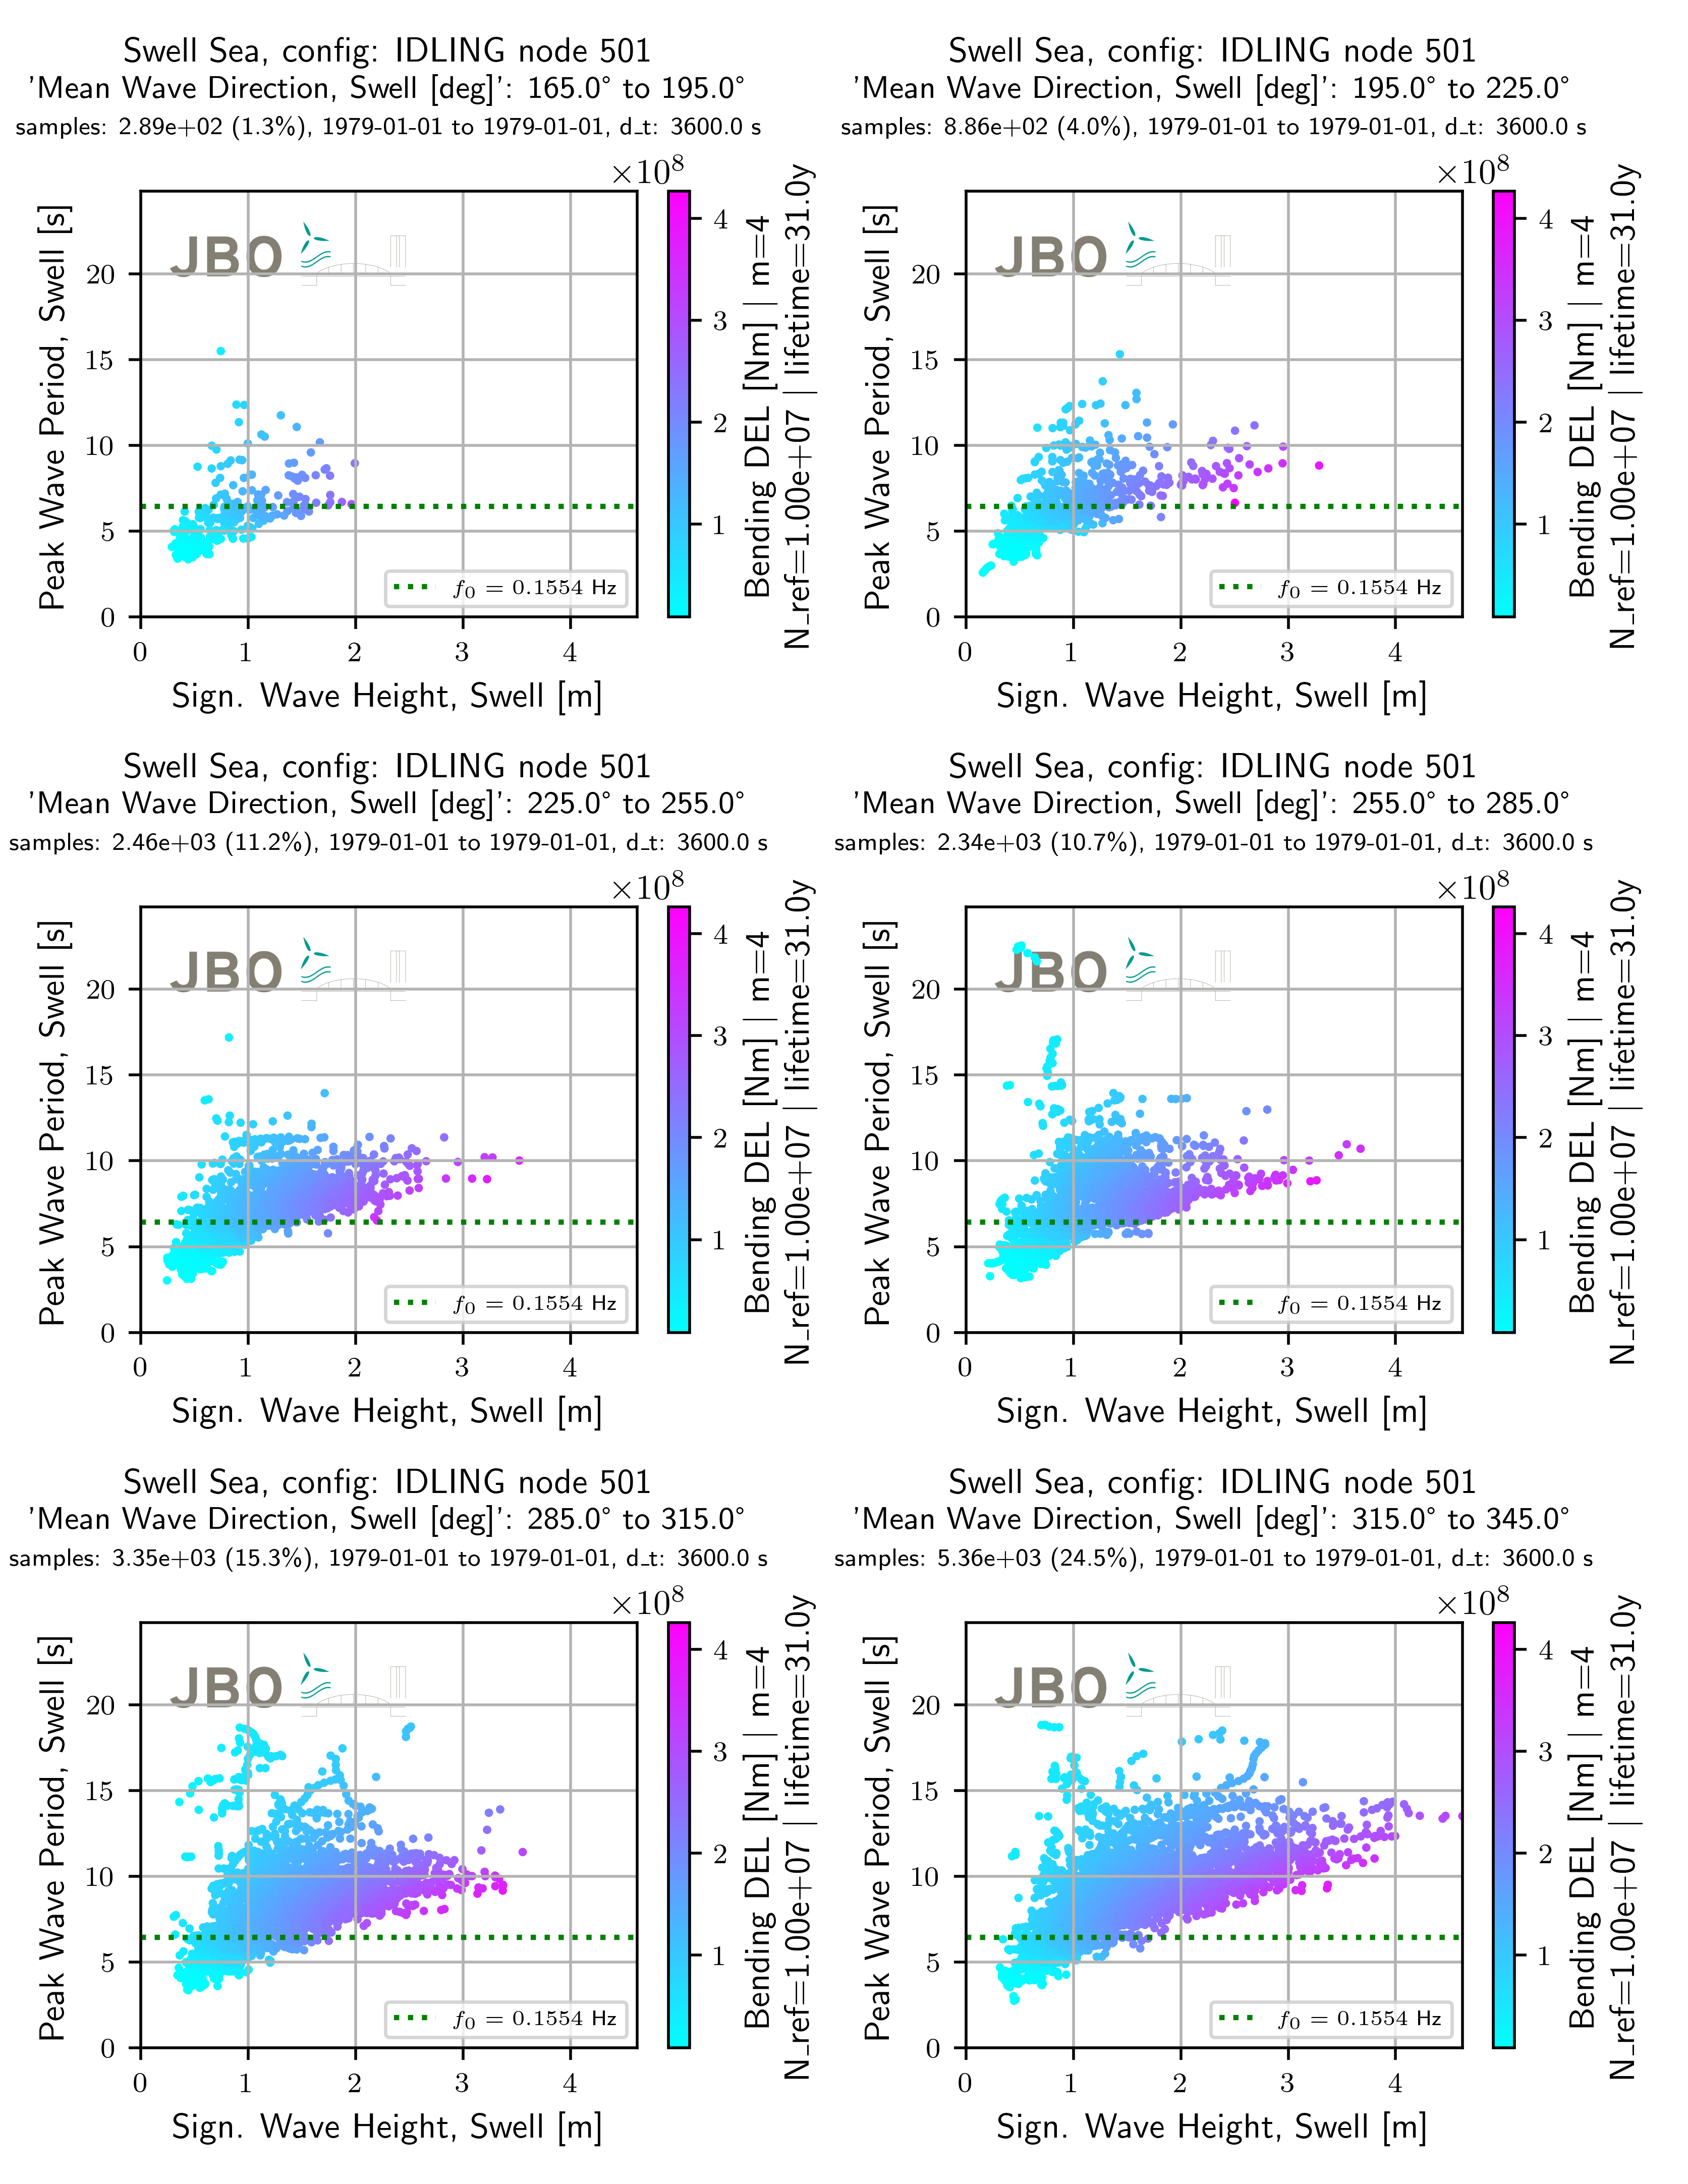
\includegraphics[width=1.0\textwidth]{C:/Users/aaron.lange/Desktop/Projekte/Hindcast_Tool/HindTool/example_output/Valid_scatter_swell_page_2.png} 
 \caption{ Valid-scatter-swell-page-2 } 
 \label{fig: Valid_scatter_swell_page_2 } 
\end{figure}